%% Template for IBK Report, or ETH Zurich Doctoral/Master Thesis 
%% Pedro Palma, IBK, ETH Zurich 
%% 2016-03-06 

%% ---------------------------------------------------------
%% ---------------------------------------------------------
%% PREAMBLE 
%% ---------------------------------------------------------
%% ---------------------------------------------------------

% ----------------------------------------------------------
% Document class 
\documentclass[a4paper, twoside, 11pt]{report}
    % specifies the type of document to be created. 

% ----------------------------------------------------------
% Character encoding 
\usepackage{mathptmx}
\usepackage[T1]{fontenc}
    % {fontenc} package allows the user to select font encodings, and for each encoding provides an interface to ‘font-encoding-specific’ commands for each font (it enables hyphenation to operate on texts containing any character in the font). 
\usepackage[utf8] {inputenc}
    % {inputenc} package allows the user to directly input accented and other characters (it translates various standard and other input encodings into a ‘LaTeX internal language'). age'). 
\usepackage{mathptmx}

% ----------------------------------------------------------
% Languages 
\usepackage[ngerman, english]{babel}
    % {babel} package manages culturally-determined typographical (and other) rules, and hyphenation patterns for a wide range of languages used languages; the last language in the option list will be active. 

% ----------------------------------------------------------
% Margins 
\usepackage[
    inner=2.5cm,
    outer=2.5cm,
    top=1.5cm,
    bottom=1.5cm,
    footskip=1.0cm,
    includeheadfoot]
    {geometry}    % {geometry} package allows to specify the 4 margins without needing to remember the particular page dimensions commands. 

% ----------------------------------------------------------
% Indent first paragraph after section header 
%\usepackage{indentfirst}    % {indentfirst} package makes the first line of all sections etc., be indented by the usual paragraph indentation. 

% ----------------------------------------------------------
% Penalties for line or page breaking 
% (penalties are the main values that TeX tries to minimise when line or page breaking; value 10000 means "disable this feature")
\hyphenpenalty=200    % the penalty for line breaking at an automatically inserted hyphen
\exhyphenpenalty=5000    % the penalty for line breaking at an explicit hyphen 

% ----------------------------------------------------------
% Coloured text 
\usepackage{color}    % {color} package allows to set the font color, the text background, or the page background; {\color{declared-color} some text} will write coloured text, \colorbox{declared-color}{some text} will enter a background colour, and \colorbox{declared-color1}{\color{declared-color2}text} will set the background and the text colour. 

% ----------------------------------------------------------
% Highlighting 
\usepackage{soul}    % {soul} package provides hyphenatable spacing out (letterspacing), underlining and some derivatives such as over striking and highlighting; \hl{some text} will highlight 'some text'. 

% ----------------------------------------------------------
% Floating objects (e.g. figures and table) 
\usepackage{float}    %  {float} package improves the interface for defining floating objects such as figures and tables. Introduces the boxed float, the ruled float and the plaintop float. You can define your own floats and improve the behaviour of the old ones. 

% ----------------------------------------------------------
% Graphics 
\usepackage[
    pdftex]
    {graphicx}    % {graphicx} is the `extended' or `enhanced' {graphics} package and it accomdates all needs for inclusion of graphics in LaTeX documents; the [pdftex] option (default if compiling with pdflatex) should be passed if you are compiling with pdftex to get a PDF that you will see with any PDF viewer. 
\usepackage{grffile}    % {grffile} extends the file name processing of package {graphics} to support a larger range of file names. 

% ----------------------------------------------------------
% Tables 
%\usepackage{tabu}    % The package provides a single environment, tabu, which will make any sort of tabular (that doesn't need to split across pages). The package requires the array package, and needs e-TeX to run (since array.sty is present in every conforming distribution of LaTeX, and since every publicly available LaTeX format is built using e-TeX, the requirements are provided by default on any reasonable system). The tabu environment may be used in place of tabular, tabular* and tabularx environments, as well as array in maths mode. It overloads tabularx's X-column specification, allowing a width specification, alignment (l, r, c and j) and column type indication (p, m and b). \begin{tabu} to <dimen> specifies a target width, and \begin{tabu} spread <dimen> enlarges the environment's "natural" width.
\usepackage{booktabs}    % Publication quality tables in LaTeX. The package enhances the quality of tables in LaTeX, providing extra commands as well as behind-the-scenes optimisation.  
\usepackage{multirow}    % {multirow} package allows creating tabular cells spanning multiple rows. 
\usepackage{array}    % {array} package is an extended implementation of the array and tabular environmentswhich extends the options for column formats, and provides "programmable" format specifications.
\usepackage{hhline}    % {hhline} package produces a line like \hline, or a double line like \hline\hline, except for its interaction with vertical lines.
\usepackage{tabularx}    % {tabularx} package implements a version of the tabular environment in which the widths of certain columns are calculated so that the table is is a specified width. 
%% Define new column types
%% (based on https://en.wikibooks.org/wiki/LaTeX/Tables#The_tabularx_package)
%% The column types defined below (L, C, and R) take their width as argument and do the following:
%%  - issue \raggedright, \centering, or \raggedleft to achieve the desired horizontal alignment;
%%  - declare \let\newline\\ to allow to use \newline for manual line breaks within a cell (note that \centering & friends change the meaning of \\);
%%  - issue \arraybackslash (i.e., \let\\\tabularnewline) to allow (again) to use \\ for ending rows,
%%  - issue \hspace{0pt} to allow the first word in a cell to be hyphenated.
%% In the definition below, the new column types are based on (vertically centered) m-columns, but one may use (top- or bottom-aligned) p- or b-columns as well.
%\newcolumntype{L}[1]{>{\hsize=#1\hsize\raggedright\arraybackslash}X}
%\newcolumntype{R}[1]{>{\hsize=#1\hsize\raggedleft\arraybackslash}X}
%\newcolumntype{C}[1]{>{\hsize=#1\hsize\centering\arraybackslash}X}

% ----------------------------------------------------------
% Captions 
\usepackage{caption}     % {caption} package provides many ways to customize the captions in floating environments like figure and table. 
\captionsetup{margin=0.0cm}
\captionsetup{labelformat=default}    % options are 'default', 'empty', 'simple', 'brace', 'parens', or user defined. 
\captionsetup{labelfont={bf,footnotesize}}    % options (list of comma separated font options if more than one; if only one of these options is used, braces can be omitted) are 'scriptsize', 'footnotesize', 'small', 'normalsize', 'large', 'Large', 'normalfont', 'up', 'it', 'sl', 'sc', 'md', 'bf', 'rm', 'sf', 'tt', 'singlespacing', 'onehalfspacing', 'doublespacing', 'stretch=<amount>', 'normalcolor', 'color=<colour>', 'normal', or user defined. 
\captionsetup{labelsep=period}    % options are 'none', 'colon', 'period', 'space', 'quad', 'nweline, 'endash', or user defined. 
\captionsetup{textfont=footnotesize}    % same options as for 'labelfont'. 

\usepackage{subcaption}    % {subcaption} package provides a means of using facilities analagous to those of the caption package, when writing captions for subfigures and the like. 
\captionsetup{belowskip=0pt}    % space between caption and content (figure or table) can be adjusted with the 'caption' package, using the arguments 'belowskip' and 'aboveskip'. Below and above have the meaning as it would make sense for figure captions below a figure: 'aboveskip' is the space between the content and the caption (which would be above the caption for a figure caption that's set underneath the figure, but below it for a table caption that's set above the table), belowskip is the space between the caption and the surrounding text.
\captionsetup[subfigure]{labelfont=bf,textfont=footnotesize,singlelinecheck=on,justification=raggedright}
% ----------------------------------------------------------
% Equations and mathematical symbols 
\usepackage{amsmath}    % {amsmath} package provides miscellaneous enhancements for improving the information structure and printed output of documents containing mathematical formulas. 
\usepackage{mathtools}    % {mathtools} package provides many useful tools to enhance the appearance of documents containing a lot of mathematics.
\usepackage{amssymb}    % {amssymb} package provides an extended symbol collection. 
%\usepackage{amsfonts}    % {amsfonts} package is automatically loaded by {amssymb} package. 

% ----------------------------------------------------------
% Other symbols 
\usepackage{textcomp}    % {textcomp} package allows to use the degree symbol ° directly. 
\usepackage{wasysym}     % {wasysym} package allows to use the diameter symbol
% ----------------------------------------------------------
% Date and time 
\usepackage{datetime}    % {datetime} package provides various different formats for the text created by the command \today, and also provides commands for displaying the current time (or any given time), in 12-hour, 24-hour or text format. 
\yyyymmdddate    % redefines \today to produce the current date displayed in the form 2000/03/08. 
\renewcommand{\dateseparator}{-}

%% ----------------------------------------------------------
%% Indexing (e.g. for Nomenclature) 
\usepackage{makeidx}

% ----------------------------------------------------------
% Chapter title style 
\usepackage{titlesec}    % {titlesec} package allows to customize chapters, sections and subsections style. 

% Change 'Chapter X \n Chapter title' to 'X. Chapter title' 
\titleformat{\chapter}
    {\normalfont\huge}
    {\textbf{\thechapter.}}{20pt}{\huge\textbf}

% ----------------------------------------------------------
% Table of contents 
\usepackage[nottoc]{tocbibind}    % {tocbibind} includes the bibliography in the table of contents. 

% ----------------------------------------------------------
% Header and footer 
\usepackage{fancyhdr}    % this package provides several commands that allow customizing the header and footer. 
\pagestyle{fancy}    % \pagestyle{fancy} sets the "fancy" style. 
\fancyhf{}    % \fancyhf{} clears the header and footer, otherwise the elements of the default "plain" page style will appear. 

% Header style 
\fancyhead[LE]{\footnotesize\leftmark}    % \fancyhead and \fancyfoot are used to customize the header and the footer in double-sided documents; the selectors that can be passed, inside brackets, are 'E' for even page, 'O' for odd page, 'L' for left side, 'C' for centered, and 'R' for right side (e.g. \fancyhead[LE,RO]{Share\LaTeX} will print the text "ShareLaTeX" on the Left side of the header for Even pages, and the Right side for Odd pages). 
\fancyhead[RO]{\footnotesize\rightmark}
\renewcommand{\chaptermark}[1]{\markboth{\thechapter.\ #1}{}}    % inserts chapter number and name ("#. Chapter name"). 
\renewcommand{\sectionmark}[1]{\markright{\thesection.\ #1}}    % inserts section number and name ("#.# Section name"). 
\renewcommand{\headrulewidth}{0.0pt}    % decorative line can be changed by increasing/decreasing its thickness (0pt means no line). 
\setlength{\headheight}{15pt}    % \headheight needs to be 13.6pt or more, otherwise you will get a warning and possibly formatting issues. 

% Footer style 
\fancyfoot[RO,LE]{\footnotesize\thepage}    % inserts page number. 
%\fancyfoot[LO]{\footnotesize\yyyymmdddate\today , \currenttime}    % inserts date and time on the left side of odd pages (YYYY-MM-DD, hh:mm). 
%\fancyfoot[RE]{\footnotesize\currenttime , \yyyymmdddate\today}    % inserts date and time on the right side of even pages (hh:mm, YYYY-MM-DD). 
\renewcommand{\footrulewidth}{0.0pt}    % decorative line can be changed by increasing/decreasing its thickness (0 pt means no line). 

% ----------------------------------------------------------
% Header and footer 
\usepackage{emptypage}    % {emptypage} makes Make empty pages really empty. It prevents page numbers and headings from appearing on empty pages. 

% Header and Footer chapter page
\fancypagestyle{plain}{% % 
	\fancyhf{} 
	\fancyfoot[LE,RO]{\thepage} % same placement as with page style "fancy"
	\renewcommand{\headrulewidth}{0pt}}

% ----------------------------------------------------------
% Widows and orphan lines 
\clubpenalty = 500    % this parameter specifies how important it is to avoid orphan lines (first words/lines of a paragraph at the end of a page); default is 150, increasing the value (e.g. to 500) makes it more important, and if set to 10000 or more it completely eliminate orphans lines. 
\widowpenalty = 500    % this parameter specifies how important it is to avoid widow lines (last words/lines of a paragraph that appear at the top of a page); default is 150, increasing the value (e.g. to 500) makes it more important, and if set to 10000 or more it completely eliminate orphans lines. 

% ----------------------------------------------------------
% Bibliography 
%\usepackage[backend=bibtex,style=numeric]{biblatex}
%\usepackage[style=alphabetic,citestyle=authoryear]{biblatex}
\usepackage[natbib=true,backend=biber,maxnames=2,sorting=none]{biblatex}
%\renewcommand\nameyeardelim{, }


% Database (path to the *.bib file) 
\addbibresource{Literature.bib}

% Replace 'Bibliography' to 'References' 
\DefineBibliographyStrings{english}{bibliography = {References},}

% Increase vertical spacing bibliography entries 
\setlength\bibitemsep{1.2\itemsep}

\usepackage{csquotes}    % this package provides advanced facilities for in-line and display quotations; useful with {biblatex}. 

% ----------------------------------------------------------
% Nomenclature 
\usepackage[
    intoc]    % [intoc] option adds the Nomenclature to the table of contents. 
    {nomencl}    % {nomencl} package produces formated lists of symbols (e.g. anomenclature) using the capbilities of the MakeIndex program. 
\makenomenclature    % \makenomenclature command is required to generate the nomenclature file (*.nlo); commenting it out is a convenient way to switch it off. 

% Group symbols depending on their type 
\usepackage{ifthen}
  \renewcommand{\nomgroup}[1]{%
  \item[\bfseries
  \ifthenelse{\equal{#1}{A}}{Latin upper-case letters}{%
  \ifthenelse{\equal{#1}{B}}{Latin lower-case letters}{%
  \ifthenelse{\equal{#1}{C}}{Greek upper-case letters}{%
  \ifthenelse{\equal{#1}{D}}{Greek lower-case letters}{}}}}%
  ]}

% Change title and add preliminary text 
%\renewcommand{\nomname}{Symbols}    % changes the default title ('Nomenclature'). 
\renewcommand{\nompreamble}{Unless otherwise specified in the text, the abbreviations and symbols have the meaning indicated below.}    % inserts some text in between the title and the list symbols. 

% ----------------------------------------------------------
% Appendices 
\usepackage[
    titletoc]    %  this option adds a name (e.g., 'Appendix') before each appendix listed in the ToC; the name is given by the value of \appendixname. 
    {appendix}    % {appendix} package provides some facilities for modifying the typesetting of appendix titles. 

% ----------------------------------------------------------
% Footnotes 
\usepackage[
    bottom]    % this option forces footnotes to the bottom of the page (the normal output routine performed by LaTeX typesets footnotes above bottom floats, which sometimes means that there could be a figure and/or a table below the footnote). 
    {footmisc}    % {footmisc} package allows changing the the typesetting of footnotes. 

% ----------------------------------------------------------
% Enumerate and itemize 
%\usepackage{paralist}    % {paralist} package provides enumerate and itemize environments that can be used within paragraphs to format the items either as running text or as separate paragraphs with a preceding number or symbol. 

% ----------------------------------------------------------
% Generated PDF files 
\usepackage[
pdftex]
{hyperref}    % {hyperref} enables to create hyperlinks within the document. 

\hypersetup{    % information entries (pdftitle, pdfauthor, ...) should be set after the package is loaded. 
    pdfauthor   = {Urias Morf},
    pdftitle    = {Optimisation of Network Tied-Arch Bridges},
    pdfsubject  = {Master's Thesis},
    pdfkeywords = {},
    colorlinks  = false}

% ----------------------------------------------------------
% Text spacing 
\usepackage{setspace}    % {setspace} package provides support for setting the spacing between lines in a document
\setstretch{1.1}    % line spacing of body text and bibliography. 
\captionsetup[table]{font={stretch=1.1}}    % line spacing of table captions. 
\captionsetup[figure]{font={stretch=1.1}}    % line spacing of table captions. 

% ----------------------------------------------------------
% Cross-references
%\usepackage{cleveref}    % {cleveref} package enhances LaTeX's cross-referencing features, allowing the format of references to be determined automatically according to the type of reference. The formats used may be customised in the preamble of a document. The package also offers a means of referencing a list of references, each formatted according to its type. In such lists, it can collapse sequences of numerically-consecutive labels to a reference range. Care must be taken when using {cleveref} in conjunction with other packages that modify LaTeX’s referencing system. Basically, {cleveref} must be loaded last...
\hypersetup{
	colorlinks   = true,  %Colours links instead of ugly boxes
	urlcolor     = black, %Colour for external hyperlinks
	linkcolor    = black, %Colour of internal links
	citecolor    = black  %Colour of citations
}

\usepackage[capitalise,nameinlink,noabbrev]{cleveref}
\creflabelformat{equation}{#2#1#3}

\newtagform{noparen}{}{}
\usetagform{noparen}
\usepackage[section]{placeins}
\makeatletter
\AtBeginDocument{%
	\expandafter\renewcommand\expandafter\subsection\expandafter{%
		\expandafter\@fb@secFB\subsection
	}%
}
\makeatother
% ----------------------------------------------------------
% Extra
\usepackage{wrapfig}
\usepackage{enumitem}
\usepackage{cases}
\usepackage{printlen} %print length of texwidth
\usepackage[export]{adjustbox} %align figure left, right
\usepackage{bm}
\usepackage{multicol}
\usepackage{gensymb}
\usepackage{siunitx}

%% ---------------------------------------------------------
%% ---------------------------------------------------------
%% DOCUMENT 
%% ---------------------------------------------------------
%% ---------------------------------------------------------

\begin{document}
\raggedbottom 			% doesn't stretch pages with little content (instead of clear page)
\setlength{\parindent}{0.0cm} 	% sets indent space for whole document

%% ---------------------------------------------------------
%% TITLE PAGE 
%% ---------------------------------------------------------

\thispagestyle{empty}    % \thispagestyle changes the style for the current page only; {empty} produces empty heads and feet - no page numbers. 

\thispagestyle{empty}
\begin{flushleft}
      
\includegraphics[scale=0.03]{Pictures/eth_logo_lang_pos.jpg} \\*[5cm]
\end{flushleft}

\begin{center}
    {\huge\rm Master's Thesis Autumn Semester 2020} \\*[0.3cm]
    \rule{\textwidth}{3pt}\vspace*{-\baselineskip}\vspace*{2pt}\\*[1cm] 	%Thick horizontal line
    {\huge\rm \textbf{Optimisation of Network Tied-Arch Bridges }}\\*[0.5cm]
    {\huge\rm Hanger Density}\\*[0.5cm]	
    \rule{\textwidth}{3pt}\vspace*{-\baselineskip}\vspace*{2pt}\\*[2cm] 	%Thick horizontal line
\end{center}

\textbf{Student:} 

Urias Morf
\vspace*{1cm}

\textbf{Supervisors:}

Georgios Klonaris

Prof. Dr. Walter Kaufmann

\vspace*{4.8cm}

\begin{wrapfigure}[3]{r}{0.4\textwidth}
\vspace{-5pt}
\hfill
\includegraphics[width=5cm]{Pictures/IBK-Logo.jpg}
\end{wrapfigure}
    
\rm ETH Zürich\\
\rm Institut für Baustatik und Konstruktion IBK\\
\rm Prof. Dr. Walter Kaufmann\\
\rm 25.01.2021

%\thispagestyle{empty}
\cleardoublepage    % \cleardoublepage ends the current page and causes all figures and tables that have so far appeared in the input to be printed; in a two-sided printing style, it also makes the next page a right-hand (odd-numbered) page, producing a blank page if necessary. 


%% ---------------------------------------------------------
%% ABSTRACT 
%% ---------------------------------------------------------
\pagenumbering{roman}
\chapter*{Abstract}
The efficient design of a network tied-arch bridge is a particular challenge due to its many design variables, such as the arch shape, the hanger arrangement and the deck system. In the last two decades, it has become a popular alternative for medium spans for road and railway bridges. Considering its efficient use of materials, a further increase is desirable. However, many aspects have not been considered in an integral and sufficient depth. Understanding the influence of the key design variables on the structural behaviour provides the basis to give general guidelines for obtaining a fast and simple initial design. 
Therefore, different hanger arrangement patterns have been developed, which have to be verified in the classical strength limit states for vehicular use and wind exposure, but also multiple extreme events and fatigue. This study aims to investigate the hanger density and its inclination further. Therefore, suitable methods for the derivation of the arch shape and the self-equilibrium stress state are necessary. In this context, the self-equilibrium stress state describes the locked-in erection stresses indirectly by the permanent supernumerary forces.\medskip

By investigating the Blennerhassett Island Bridge, optimisation potential for the hanger density and the hanger inclination is identified. Further, new methodologies for the derivation of the arch shape and the self-equilibrium stress state are introduced. For the arch shape, an approximation of the thrust line of the hypothetical continuous hanger arrangement is recommended. The self-equilibrium stress state is optimised by formulating an efficiently solvable linear programming problem. The investigation is conducted in a linear elastic single arch plane model under various strength and extreme event limit states. As a measure for the optimality, the main components' structural costs are estimated for comparative purposes. For the reference case of the Blennerhassett Island Bridge, the approximation of the arch shape to the thrust line and an optimised self-equilibrium stress state yielded considerable savings. On the other hand, the hanger density has a negligible impact on the structural behaviour besides reducing the effects in the extreme event of cable loss. Ultimately, the hanger inclination significantly changes the elastic response of the structure and the optimal arch shape.\medskip

Based on the results, new design guidelines are formulated. Primarily, the floating deck should be optimised in a first step before considering the structure of the network arch. The considerable offset of the arch's thrust line to the typical arch shapes under permanent loads is reduced by adapting the shape to the respective quartic polynomial. Further, a uniform spacing of the hanger anchorages on the arch rib is recommended to reduce the inevitable shape deviation moments. However, a uniform spacing on the tie girder is also critical, rendering the radial hanger arrangement particularly disadvantageous. An increased hanger density has to be paired with a corresponding increase in the number of floor beams. Ultimately, the constant change of inclination arrangement considerably increased the coupling of the arch rib and the tie girder. Therefore, it is recommended with substantial changes in the hangers' inclinations. These guidelines are particular to the Blennerhassett Island Bridge and its particularly large spacing of the hangers and the floor beams. Further investigations smaller bridges and composite deck systems can be investigated using the same methods and could provide promising insights.

\cleardoublepage


%% ---------------------------------------------------------
%% FOREWORD 
%% ---------------------------------------------------------
\chapter*{Foreword}

During an internship in the summer of 2018, I worked on a small pedestrian passage over a highway. It was the first new construction I was assigned to, and it was an exciting Vierendeel girder. As time was pressing and my team had substantial autonomy on the design, many decisions were made quickly and based on personal preference. Towards the end of the deadline, it seemed like we were just in time. Only then, we noticed that a specific serviceability verification could not be fulfilled. The project manager gave me the job to identify a simple change of the geometry or the cross-sections to solve the issue. However, it was a challenging task and everything I tried backfired in one way or another. Neither any of the experienced engineers found the solution we were looking for. To solve the issue once and for all, it was decided to arrange diagonal high strength steel cables in each frame. All conditions were met, and the plans were sent out shortly afterwards. But it left me unsatisfied, knowing the cables were not necessary but also feeling poorly equipped to solve the issue.\medskip

The design of a network tied-arch bridge poses many more considerable challenges: Its high degree of intrinsic static indeterminacy gives the engineer control of the flow of forces, but it also complicates understanding its structural behaviour. As the bridge-type makes advantageous use of the utilised materials, extreme events in which a component is lost can become decisive. Further, the structure's entire geometry, including the hanger arrangement and the arch shape, is negotiable. This opens up a large space of plausible solutions and makes the civil engineer's decisions have a far-reaching influence on the structure's efficiency and financial expenses. These significant challenges are partially responsible for its sparse use, despite its aesthetic appeal and structural efficiency. \medskip

The next decades pose tremendous challenges in many scientific fields, and despite not often being in the spotlight, demanding issues are facing the discipline of civil engineering. However, it seems that the method of trial and error relying on fundamental structural understanding and a handful of experience is considered sufficient for civil engineers. This feeling was accentuated by the fact that a lecture on structural optimisation was only offered at the department of mechanical engineering. However, for complicated and insufficiently investigated structures, such as a network tied-arch bridge, optimisation methods are an invaluable tool to overcome its challenges. I want to thank my supervisors, Georgios Klonaris and Prof. Dr. Kaufmann, for giving me the opportunity and the support to investigate this particularly interesting bridge type. Besides finding optimisation potential for network tied-arch bridges, I hope to contribute to the use of more advanced methods in civil engineering. A diversified toolbox does not just facilitate more efficient designs, it also increases the enjoyment of the challenge itself.
\cleardoublepage


%% ---------------------------------------------------------
%% ACKNOWLEDGEMENTS 
%% ---------------------------------------------------------
%\chapter*{Acknowledgements}

%\cleardoublepage


%% ---------------------------------------------------------
%% TABLE OF CONTENTS 
%% ---------------------------------------------------------

\begingroup
\linespread{1.2}
%	\thispagestyle{empty}
%	\addtocontents{toc}{\protect\thispagestyle{empty}} 
\pagestyle{fancy}
\tableofcontents

\cleardoublepage
\endgroup

%% ---------------------------------------------------------
%% TABLE OF FIGURES AND TABLES
%% ---------------------------------------------------------
\pagestyle{fancy}
%\fancypagestyle{plain}{%
%	\fancyhf{} % clear all header and footer fields
%}
\listoffigures
\cleardoublepage

\pagestyle{fancy}
%\fancypagestyle{plain}{%
%	\fancyhf{} % clear all header and footer fields
%}
\listoftables
\cleardoublepage

%% ---------------------------------------------------------
%% CHAPTERS
%% ---------------------------------------------------------
\pagenumbering{arabic}

\chapter{Introduction}\label{sec:intro}
In this chapter, the problem addressed by this Master Thesis is introduced. First, the bridge type and its characteristics are described in \cref{sec:int_back}, complemented by a brief historical integration. In \cref{sec:int_prob}, the problem is stated and defined. Ultimately, an outline of the Thesis and an overview of used terminology is given. in Section \ref{sec:int_out} and \ref{sec:int_term} 

\section{Background}\label{sec:int_back}
Network tied-arch bridges serve the same function as simply supported beams by spanning a single field supported on vertical bearings at its ends, of which one is horizontally restricted. Compared to a simple beam, which carries the loads on internal bending moments, the tied-arch bridge forms a truss structure featuring a tension and a compression chord to carry the global bending moment. The tie girder forms the tension chord tying the arch ends and supporting its horizontal forces. The deck may be integrated into the tie girder (composite deck system) or be supported vertically on deck floor beams (floating deck system). The arches are arranged in planes which can either be vertical or inclined. Each plane usually features two hanger sets, which connect the tie and the arch and cross each other multiple times. The structural components for a floating deck system are illustrated in Fig. \ref{fig:components_illustration}.
\begin{figure}[H]
    \centering
    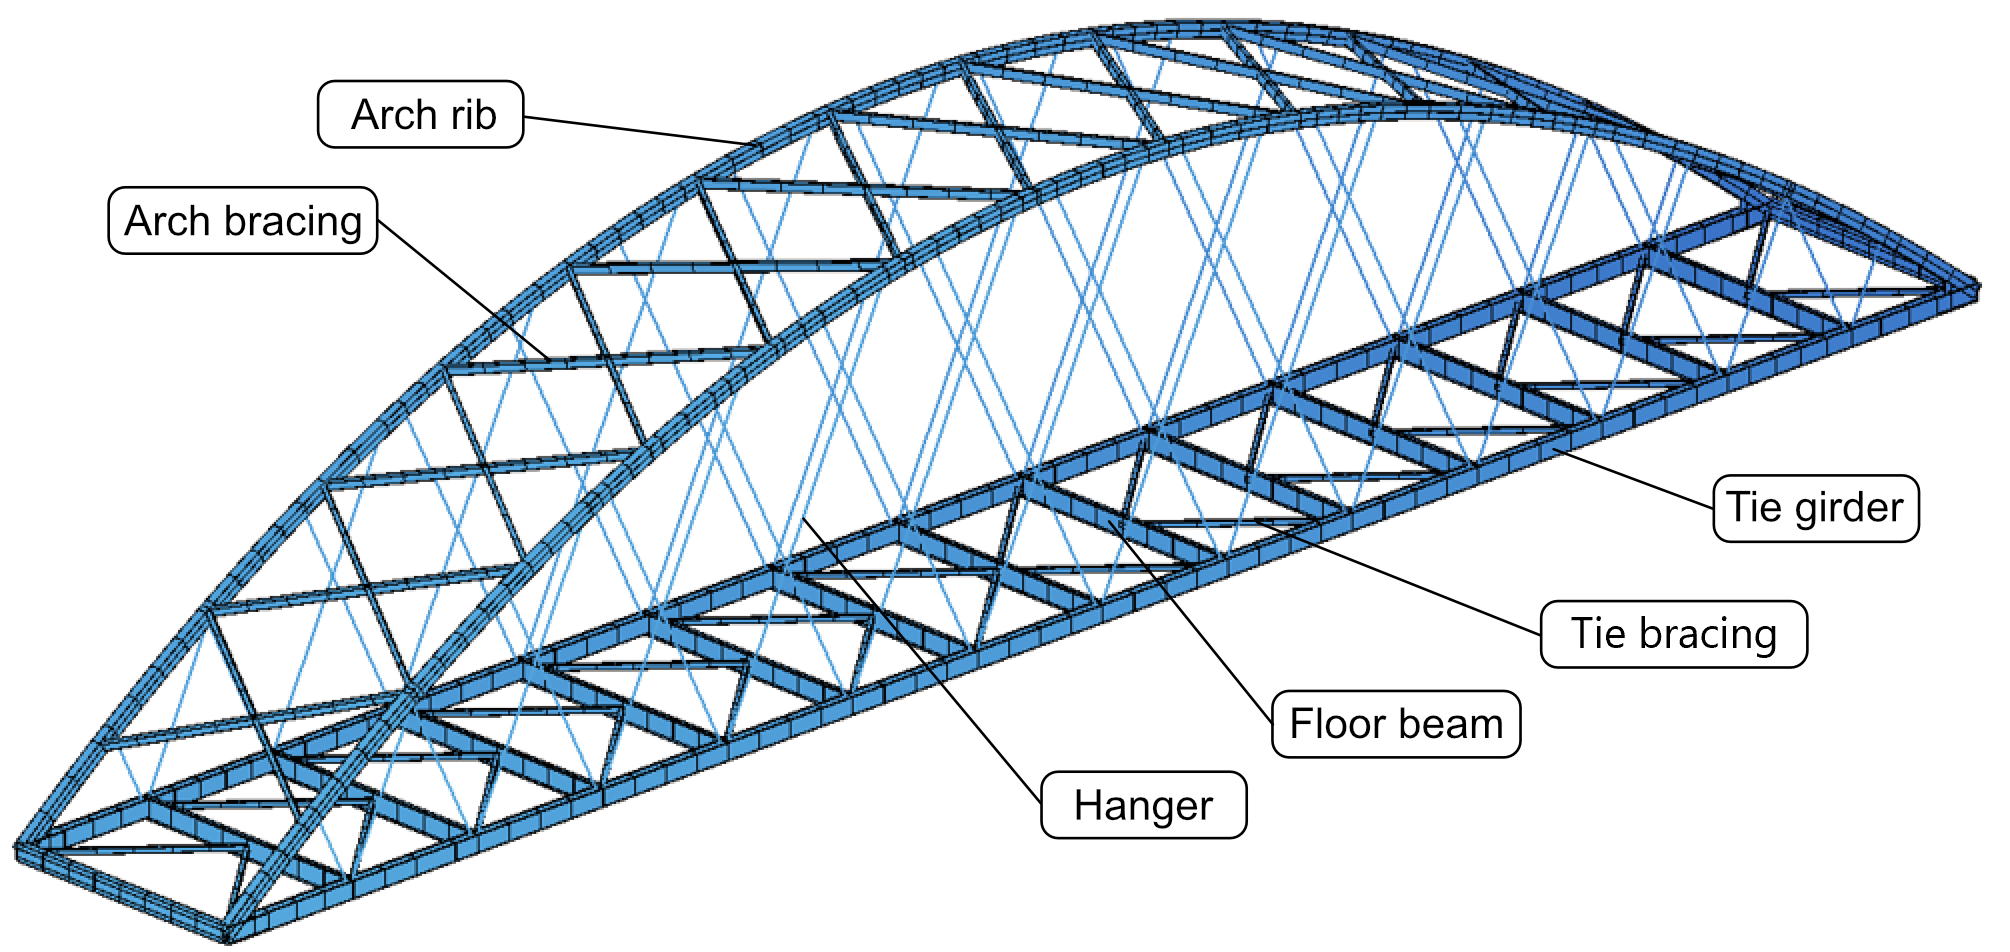
\includegraphics[width=0.65\textwidth]{overleaf/Pictures/illustration_components.PNG}
    \caption{Structural components of a network tied-arch bridge}
    \label{fig:components_illustration}
\end{figure}

The network tied-arch bridge is considered an enhanced construction scheme offering aesthetic appeal and benefits in terms of structural efficiency \cite{Hu}. Steel bridges of this type require significantly less material and allow for more slender cross-sections than other more popular bridge-types \cite{Herzog}. However, network tied-arch bridges can be considered a complex structural system and the associated challenges are broad and demanding. 
The hanger arrangement and its initial configuration influence the behaviour under asymmetric live loading, fatigue and cable loss. 
Many of these challenges have not been satisfactorily addressed \cite{Bruno_2}. Other design variables such as the arch shape and its rise as well as its bracing and inclination have barely been studied. Nevertheless, a strong surge in the popularity of this bridge-type is observed in the last two decades, as shown in \cref{fig:yearly_bridges}.

\begin{figure}[H]
    \centering
    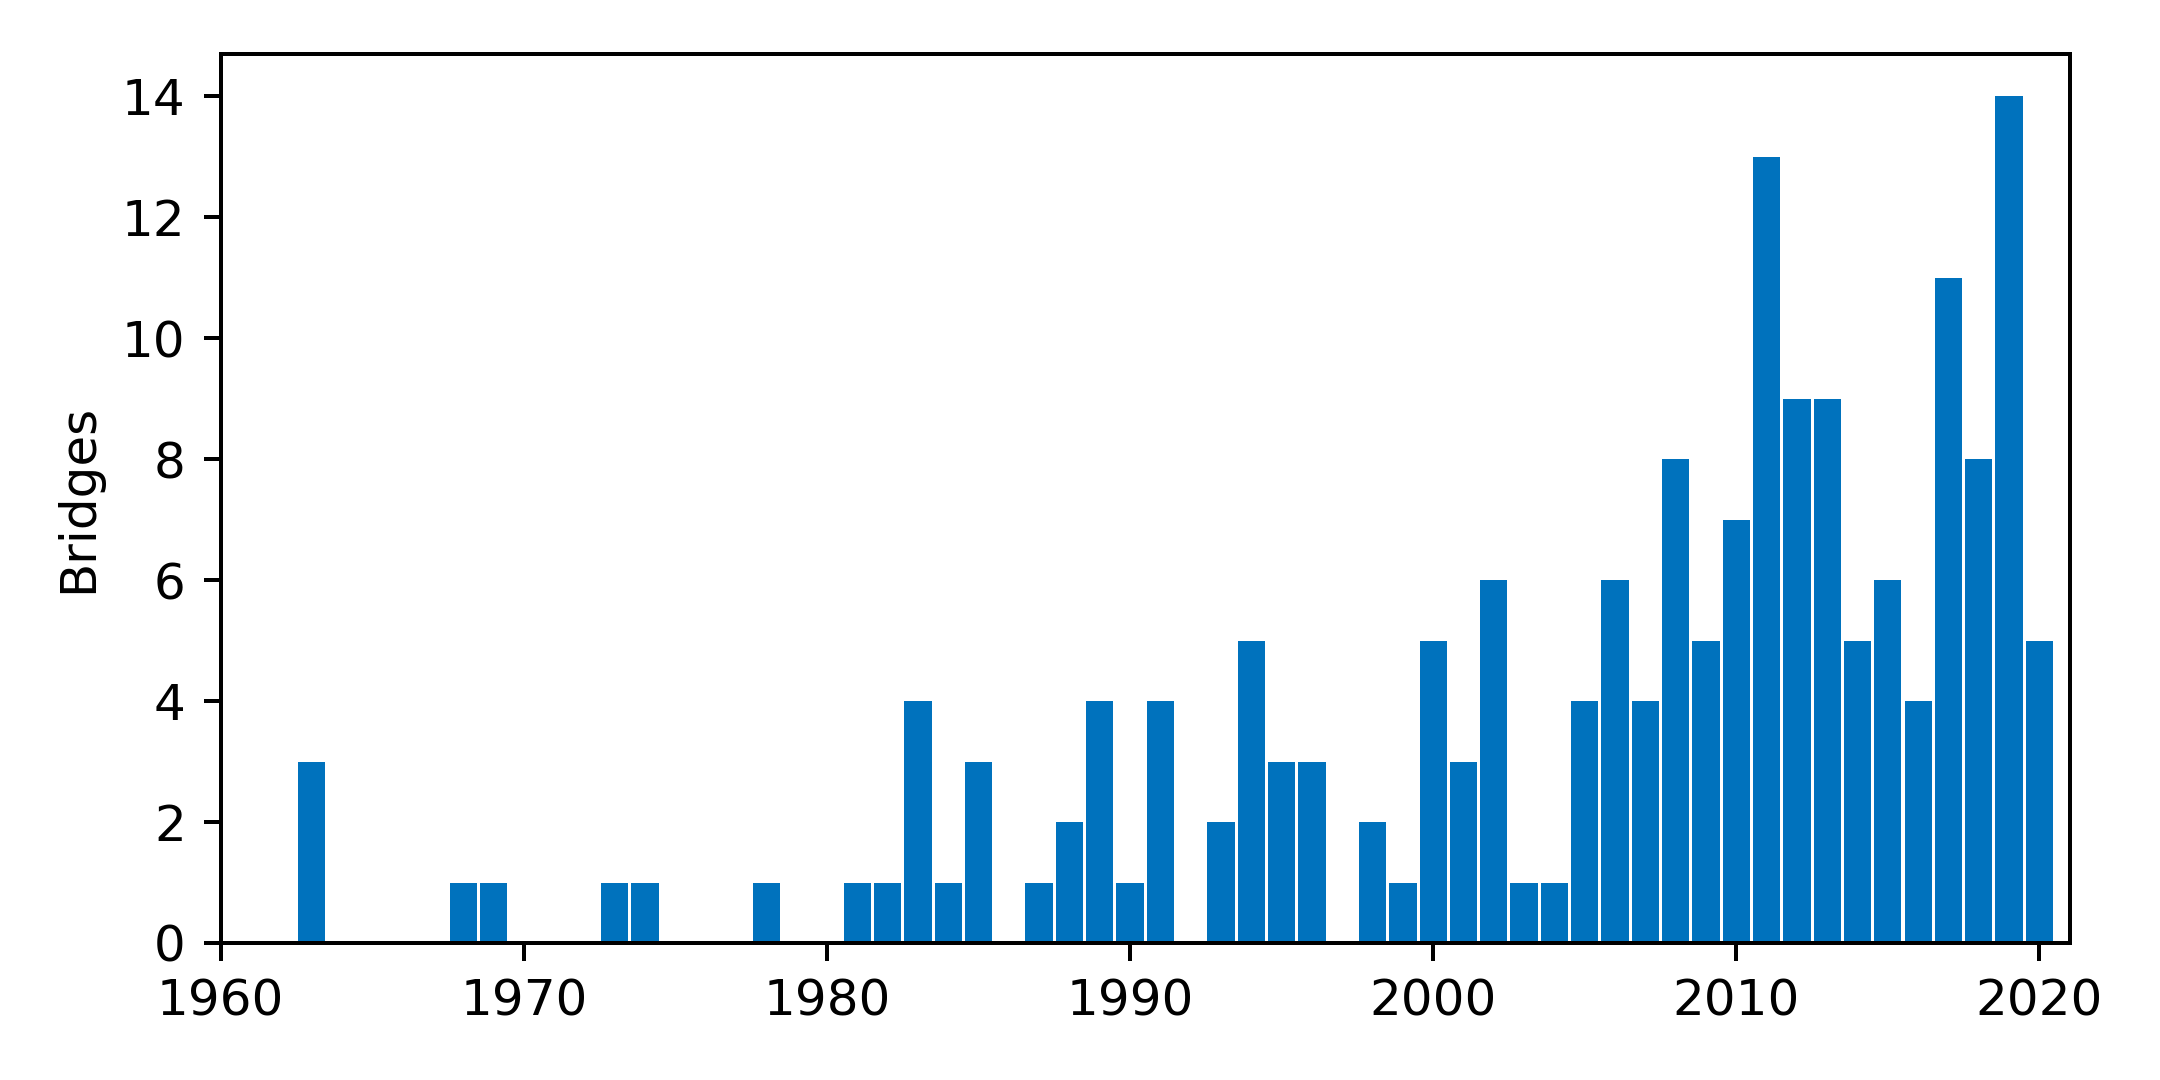
\includegraphics[trim={0 2.2cm 0 1.8cm},clip, width=0.60\textwidth]{overleaf/Pictures/myplot.png}
    \caption{Number of network tied-arch bridges built per year \cite{Cavegn}}
    \label{fig:yearly_bridges}
\end{figure}

The origin of this bridge type can be traced back into the 19th century when multiple engineers started designing tied-arch bridges featuring a tension chord in the tie. Among these engineers are Joseph Langer and Hermann Lohse who arranged the hangers vertically as shown in \cref{fig:langerscherbalken}. In the 1920s, the Danish engineer Octavius F. Nielsen recognised the advantages of inclined hangers, which significantly reduce the longitudinal bending moments and thereby allow for longer spans. Despite showing intersecting hangers in his patent document, he only designed hanger arrangements without intersections \cite{Tveit_Bits}. The structural analysis of a bridge with intersecting hangers was too challenging at the time. Besides that, he struggled with hanger loss due to unloading. One of his bridges is presented in Fig. \ref{fig:nielsenbridge}.

\begin{figure}[H]
\centering
\begin{minipage}{.5\textwidth}
  \centering
  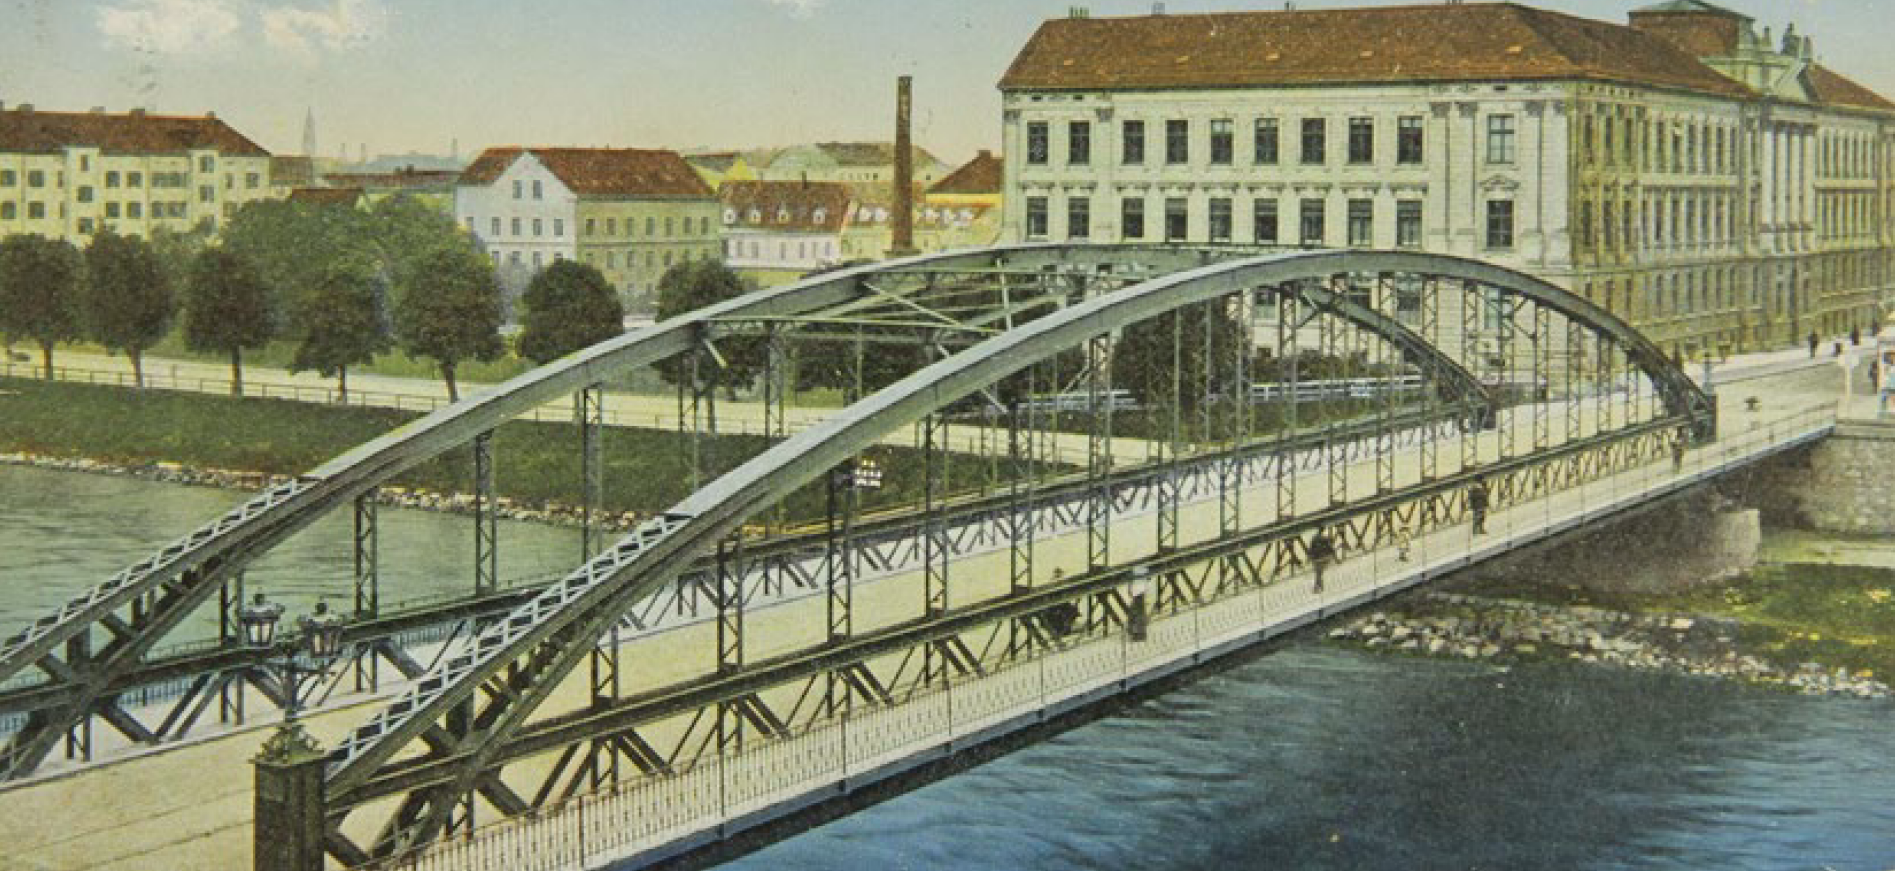
\includegraphics[width=.9\textwidth]{overleaf/Pictures/langerscher balken.PNG}
  \captionof{figure}{Old Ferdinandbridge \cite{Langer}}
  \label{fig:langerscherbalken}
\end{minipage}%
\begin{minipage}{.5\textwidth}
  \centering
  \vspace*{0.6cm}
  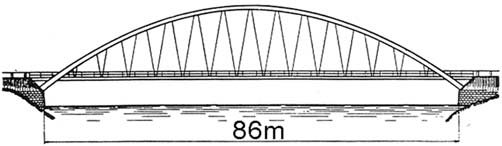
\includegraphics[width=.9\textwidth]{overleaf/Pictures/Nielsen bridge.png}
  \vspace*{0.6cm}
  \captionof{figure}{Nielsen bridge \cite{Nielsen}}
  \label{fig:nielsenbridge}
\end{minipage}
\end{figure}

As the live loading increased in the following years, Nielsen bridges became less suitable. Only by intersecting the hangers, flat hanger inclinations could be obtained, which solves the problem of hanger unloading. The network tied-arch bridge featuring hangers with multiple intersections was introduced by Per Tveit in 1955. The first bridges of this type were built in 1963. One of them, the Fehmarn Sound Bridge, which already spanned \SI{248}{m}, is shown in \cref{fig:Fehmarnsundbrcke}.

\begin{figure}[H]
    \centering
    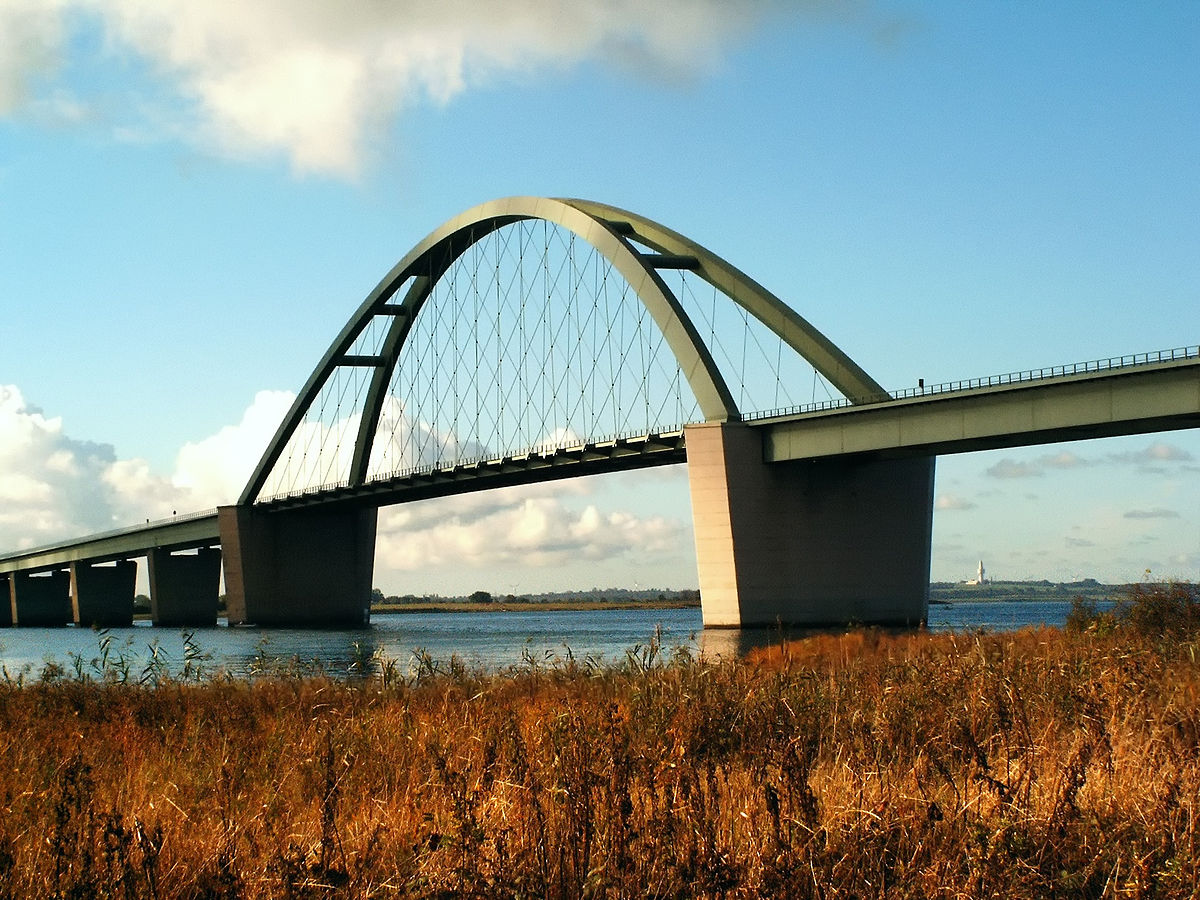
\includegraphics[trim={0 1.5cm 0 0.7cm},clip, width=0.55\textwidth]{overleaf/Pictures/Fehmarnsund.jpg}
    \caption{Fehmarn Sound Bridge \cite{Fehmarnsund}}
    \label{fig:Fehmarnsundbrcke}
\end{figure}

In the following decades, Per Tveit focused his research on this bridge type, emphasising the importance of the hanger inclination. Despite his efforts, no more bridges of this type were built in Europe until the end of the millennium. However, the idea was exported to Japan, where it became a standard alternative to classic tied-arch bridges and over 50 bridges of this type were built for medium spans. In the last two decades, researchers and engineers developed more interest in this bridge type, which has now been built more than 200 times around the world. The Blennerhassett Island Bridge, shown in \cref{fig:Blennerhassett}, is a particularly large example, which serves as a reference for the investigations in this Thesis.

\begin{figure}[H]
    \centering
    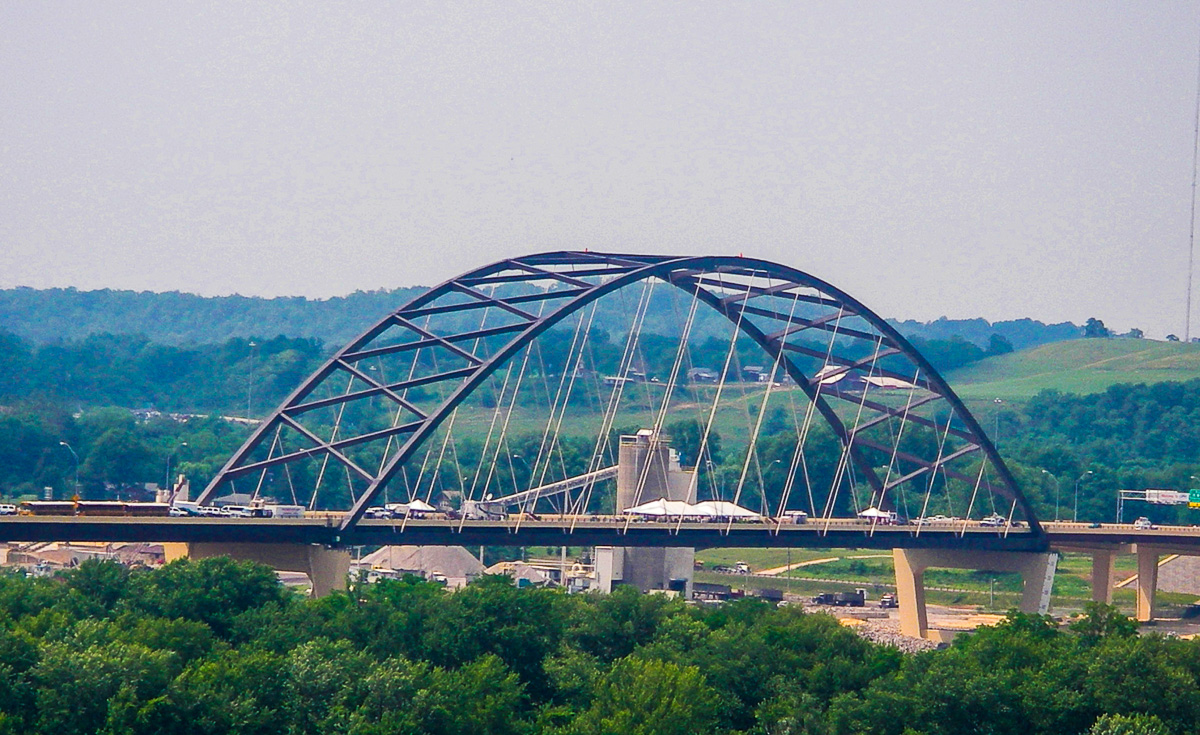
\includegraphics[width=0.6\textwidth]{overleaf/Pictures/Blennerhassett.jpg}
    \caption{Blennerhassett Island Bridge \cite{Blennerhassett}}
    \label{fig:Blennerhassett}
\end{figure}

\section{Problem statement} \label{sec:int_prob}
This Master Thesis is part of a series of projects on network tied-arch bridges at the institute of structural engineering at ETH Zurich. As the full optimisation of this bridge type covers too many aspects for a single Thesis, different focal points are investigated independently. A previous Master Thesis carried out by Riccardo Cavegn investigated the arch geometry, the optimal determination of the initial configuration (self-equilibrium stress state) and the hanger inclination. The present Thesis relies on this previous work and faces many identical challenges. Again, the hangers are subject to the optimisation in this Thesis as they determine this bridge-type's fundamental behaviour. In particular, the emphasis lies in the investigation of the hanger density and its related aspects. The Blennerhassett Island Bridge serves as a reference for the investigations. It is an impressive structure which was designed mainly for structural efficiency, which frames the objective in this Thesis.  
%Along with the hanger arrangement, the hanger density is the key parameter determining the fundamental behaviour of this bridge type.\\

\section{Outline} \label{sec:int_out}


\section{Terminology} \label{sec:int_term}
[Hanger inclination]
[Hanger set] Two symmetrical hanger sets
[Hanger arrangements] The hangers follow a certain order. 
[Knuckle]
[zero-displacement method]
[Hanger orientation, left, right]
Objective function: Most optimisation methods require the definition of a single function to rank the optimality of a specific design. The optimisation method tries to find design which yields the minimum value for this function.
[Design condition:]
Self equilibrium stress state
Arch shape

\cleardoublepage

\chapter{Literature review}\label{sec:review}
In this chapter, previous work on the optimisation of network tied-arch bridges related to the introduced problem is summarized. However, the field is rather young in general, and further, most emphasis has been placed on the hanger arrangement pattern over the density. Nevertheless, the studies on the hanger arrangement pattern are of relevance to this Thesis, as the density is linked to the arrangement and the same methods are suitable for either investigation. In most studies, a single aspect is investigated, such as hanger unloading or the hanger forces in general, fatigue or cable loss. These aspects, which are investigated in parametric studies, are introduced in Sections \ref{sec:rev_forces} to \ref{sec:rev_loss}. Besides parametric studies, numerical optimisation methods have been used not just to identify the tendencies, but to further optimise the choice of parameters in the continuous domain. Recently, these methods have been used to minimise the weight or even the costs of a network tied-arch structure. The respective studies are introduced in Sections \ref{sec:rev_weight} and [!!!]. Few authors have taken a further step and introduced a design methodology allowing for a fast and approximately optimized initial design. These methods, which are evaluated critically, are presented in Section \ref{sec:rev_meth}. Ultimately, the Master Thesis of Riccardo Cavegn, which builds the foundation of this Thesis, is summarized in Section \ref{sec:rev_prev} and a summary of this chapter is given in Section \ref{sec:rev_sum}.

\section{Hanger forces} \label{sec:rev_forces}
Per Tveit, described the concept of network tied-arch bridges in his dissertation in 1959 and designed two of the first bridges of this type in 1963 in Norway.
%[History] Since then, he has been giving lectures around the world to contribute to the broader use of network tied-arch bridges. He points out the various advantages over vertical hangers in terms of lower steel weights, simple detailing and the good use of strong materials \cite{Tveit}. He recommends constant hanger spacing on the arch with one hanger per node to minimize the bending moments in the arch. 
He also conducted investigations on the hanger arrangement, aiming to prevent hanger unloading which is a critical issue under asymmetric loading for short-span bridges \cite{Tveit3}.
In these early stages, only the parallel hanger net and the constant change of inclination pattern were used. 
It was found that whereas flat inclinations are more suitable to prevent hanger unloading, they also result in higher hanger forces. To find a solution for these opposing objectives he developed diagrams, which predict the maximum hanger inclination without hanger unloading depending on the ratio of life to dead loads. As a first optimisation of the hanger arrangement, he proposed to increase the inclinations of the hangers as much as possible before the first hanger unloading occurs. \medskip

In 2012, Teich conducted a vast parameter study varying the key in-plane parameters to investigate the hanger force-related objectives \cite{Teich}. Namely, these objectives are the maximum force, its variation, the cyclic stresses and the amount of unloaded cables, without considering the three hangers closest to the knuckle. The parameters such as the span, the rise, the amount of hangers and their arrangement are varied in the study, leading to a total of approximately \SI{90000}{} variants. The only in-plane parameter which is left constant is the circular arch shape. The cross-sections of the arch rib and the tie girder were obtained in a simplified preliminary design assuming a steel carriageway. Each variant was then analysed in a two-dimensional model under unilateral and full vertical train live loading. 
Again, hanger unloading posed a big issue for many variants and affected all investigated objectives. Therefore, Teich recommends the arrangement of 36 to 52 hangers per plane for spans between \SI{100}{m} and \SI{250}{m}. Further, he recommends flat inclinations between $50\degree$ and $55\degree$ for the parallel hanger pattern. The constant change of inclination arrangement offers significant advantages and relies on large changes of inclination. However, the radial arrangement with an intersection angle $\beta=36\degree$ was found the best regarding virtually all the considered objectives. Based on the normalized and combined objectives, Teich also developed a design methodology, which is explained in Section \ref{sec:rev_meth}. \medskip

It has to be noted, that both Tveit and Teich did not consider prestressing of the hangers in their models. It is implicitly assumed, that the permanent hanger forces correspond to the elastic response under permanent loads. Also, the ratio of live to dead loads is assumed to be particularly high (up to $p/g=1$). Therefore, the impact of hanger unloading is significantly overestimated compared to common network tied-arch bridges featuring a concrete deck.
%results normalized and mixed multiple times.

\section{Fatigue} \label{sec:rev_fat}
Pellegrino et al. evaluated hanger patterns with respect to fatigue on a bridge featuring a composite deck and a life to dead load ratio of $p/g=0.3$ and a span of \SI{100}{m} \cite{Pellegrino}. The considered hanger patterns are the constant change of inclination and the radial arrangement which are also compared to a vertical arrangement. It is found that with respect to the maximum and the average cyclic stresses, vertical hangers are advantageous over network arrangements. By inclining the vertical hangers the behaviour deteriorates strongly and improves again for flat inclinations. Especially the flat hangers of the radial arrangement near the knuckle undergo very high cyclic stresses and various modifications to reduce the maximum cyclic stress are studied. However, no generally applicable modification independent of the intersection angle was found. Therefore, it is recommended to design the hangers near the knuckle independent of the hanger arrangement pattern. Steeper hangers near the knuckles are generally a good advice to start with. For a radial hanger arrangement with 22 hangers per set, it is recommended to arrange the last five hangers of each set parallel to the previous one, as shown in \autoref{fig:Pellegrino}.
\begin{figure}[H]
    \centering
    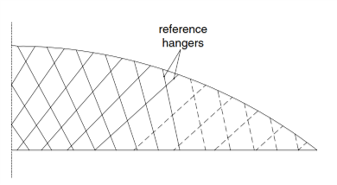
\includegraphics[width=0.5\textwidth]{Pictures/PellegrinoArrangement.png}
    \caption{Modified radial arrangement \cite{Pellegrino}}
    \label{fig:Pellegrino}
\end{figure}


\section{Cable loss} \label{sec:rev_loss}

Most of the work dedicated to cable loss focuses on cable-stayed bridges, for which it is not unusual, that the design of the superstructure is governed by this accidental limit state. Wolff and Starossek found, that the loss of two or more cables can even impair the global stability of a cable-stayed bridge \cite{Wolff}. In an investigation on the Blennerhassett Island Bridge, Zoli and Woodward showed that a network tied-arch bridge offers more redundancy and can even withstand the loss of multiple cables \cite{Zoli}. However, it is concluded that cable loss should be a key consideration for the design process for all major network tied-arch bridges. Further they point out that a detailed dynamic analysis can allow for a significant reduction of the dynamic amplification factor due to cable loss.\bigskip

Bruno et al. conducted a study on the behaviour of network tied-arch bridges to identify the key factors on the effects under cable loss \cite{Bruno}. The behaviour is studied using the simplified approaches of the PTI and the Eurocode and compared to a dynamic non-linear FE-analysis \cite{PTI}. As a reference case, a bridge with a span of \SI{180}{m} and a rise of \SI{30}{m} is studied featuring a parallel hanger arrangement with 17 hangers per set and an inclination of $65 \degree$. Further, prestressing is taken into account using the zero-displacement method. It was found that the most dangerous cables to lose are the ones located near the quarter points of the tie and are inclined towards the crown of the arch. The corresponding vertical displacements are maximal for this hanger with a value of $l/4000$. The stresses in the neighbouring hangers of the same set increase by 60\%, if the cable at the quarter point is lost. The hangers of the other set are less affected increasing by a maximum of less than 25\% as shown in Fig. \ref{fig:Bruno}. It is concluded, that also the simplified method by the PTI provide an adequate degree of accuracy, as they only underestimate the hanger forces in the less affected hanger set.
\begin{figure}[H]
    \centering
    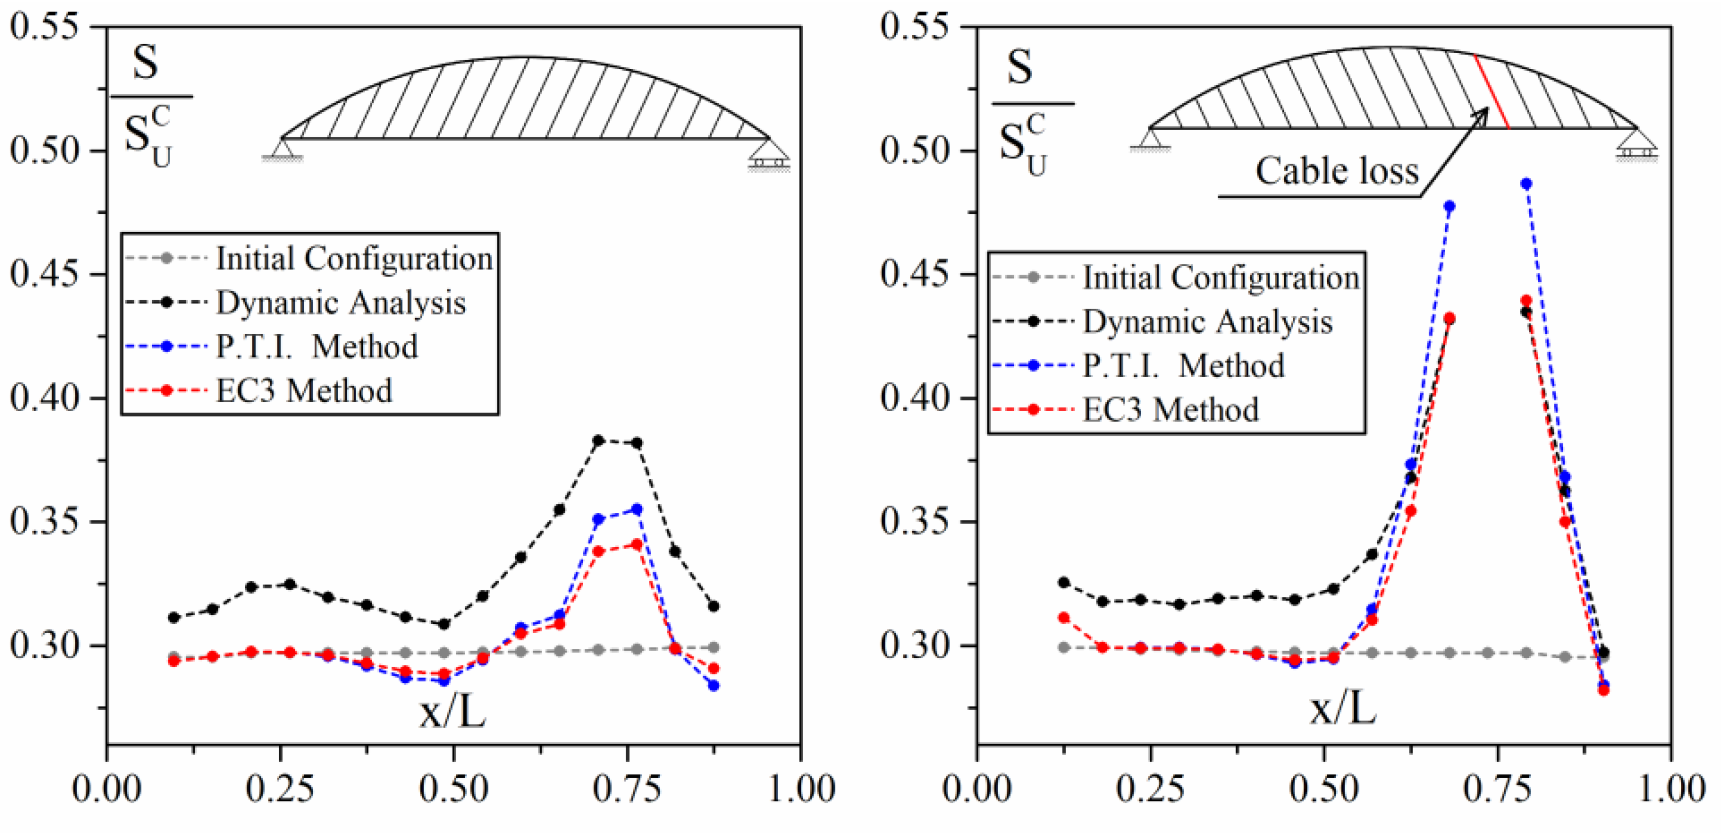
\includegraphics[width=0.75\textwidth]{Pictures/BrunoCableLoss.PNG}
    \caption{Stress distribution in the hanger sets \cite{Bruno}}
    \label{fig:Bruno}
\end{figure}

Further, it was found that parallel arrangements with flatter inclinations cause the displacements and the internal forces to increase. Restricted to the plausible range of $50\degree$ to $70\degree$, differences in the deflections amounting up to 20\% can be expected. In Fig. \ref{fig:Bruno2} the respective displacements are also compared to the arrangement with vertical hangers, where also the resulting total volumes of the hangers are given. It is seen that the vertical arrangement performs significantly better despite using a smaller quantity of cable material. Compared to the investigations on hanger forces and fatigue, an opposite tendency is observed, where the behaviour improves for steeper hangers. This is due to the stiffer behaviour of steep hangers.
\begin{figure}[H]
    \centering
    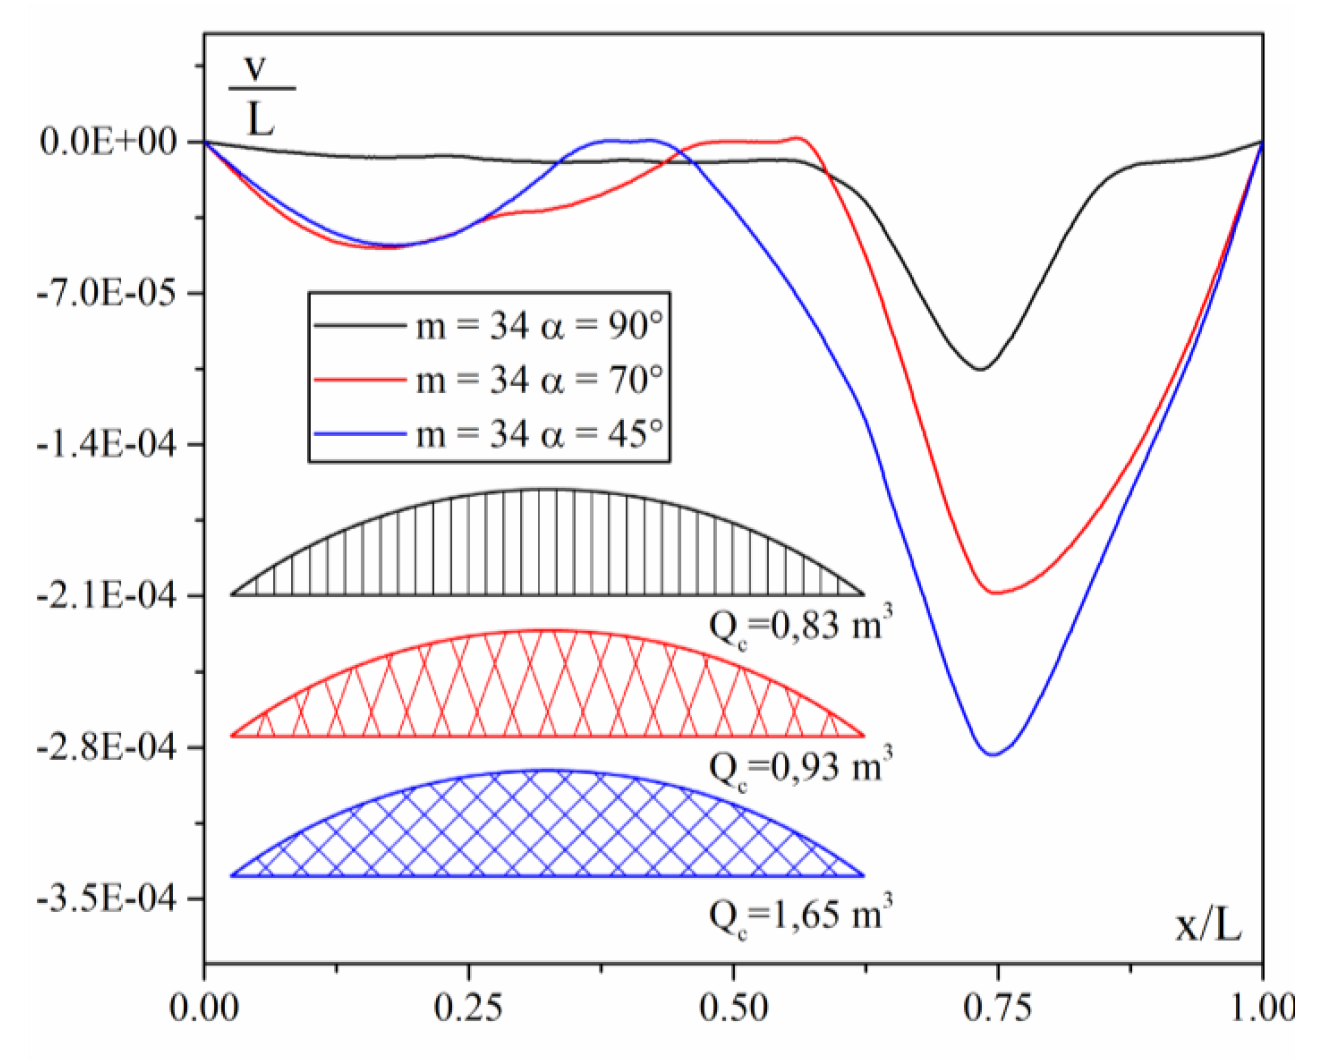
\includegraphics[width=0.6\textwidth]{Pictures/BrunoArrangements.PNG}
    \caption{Vertical deflections under cable loss \cite{Bruno}}
    \label{fig:Bruno2}
\end{figure}

\section{Structural weight} \label{sec:rev_weight}
Recently, many researchers have focused on numerical optimisation methods over parametric studies. Technically, all parameters describing the scheme of a network tied-arch bridge can be considered. However, as it is usually not the aim to optimise a full design, researchers prefer to limit the process to a few key variables. As some of the parameters are of discrete form, the problem is mathematically described as a constrained mixed-integer problem. Genetic algorithms with penalisation provide an efficient and often used tool for these problems. Belevicius et al. optimised a pedestrian bridge with respect to the weight for different boundary conditions \cite{Belevicius}. Even with the rather limited amount of nine parameters, the optimized sets are well dispersed over the feasible domain, accentuating the multi-modality of the underlying problem.
It also demonstrates the difficulties associated with numerical optimisation for design purposes. Even after reducing the amount of parameters, the results do not resemble typical tied-arch bridges, be it for the high amount of hangers or the large rise-to-span ratios. Ultimately, a strongly varying hanger pattern is recommended as well as a rise-to-span ratio of up to 0.23. The aim of finding a simple and fast method for obtaining the full initial design is therefore reached only in an unsatisfactory manner.
It is likely, that an oversimplified objective function yielded these odd designs, as the unfactored weights neglect the differences in the unit costs, which favours the arrangement of additional hangers in particular.

\section{Structural costs}
Design optimisations often take the goal of minimising the structural costs as an objective. Recently, researchers have used a wide range of optimisation methods to solve problems with geometrical, topological and mechanical design variables underlying different sets of structural constraints \cite{MARTINS}. However, the main focus of the field lies again on cable-stayed bridges, and further, only a single publication attempted to take the construction expenses into the objective. It is key to remember, that for the slender network tied-arch bridges a high ratio of the costs is made up by labor and not by the material and the fabrication of the components \cite{Tveit2}. Therefore, the estimated structural costs can serve well as a guideline, however it makes sense, to keep the focus on the structural considerations.

\section{Design methodologies} \label{sec:rev_meth}
The complex behaviour of the network tied-arch bridge is at least partially responsible for its comparably sparse use \cite{Tveit2}. As an engineer does not have the capacity to run a full optimisation, design guidelines or methodologies are key to promote the construction of this bridge type. However, only few authors have attempted to tackle this challenge for network tied-arch bridges.

Teich developed a design methodology based on the results of a vast parameter study. In a first step, the number of hangers is chosen according to the recommended values depending on the span of the bridge, shown in [Figure]. Using the amount of hangers and the span, the optimal hanger arrangement pattern is chosen using a different table, in which the arrangements are ranked according to their normalised score. For all cases either the constant change of inclination or the radial arrangement are the preferred choice. Ultimately, the best set of parameters can be chosen depending on the amount of hangers in a table corresponding to the respective hanger set. An example for the radial arrangement is shown in [Figure]. The three hangers closest to the knuckle should ultimately be designed manually. 

Whereas this methodology is fairly simple to use, it lacks a specific boundary of application. For the span of the Blennerhassett Island Bridge, a minimum amount of 42 hangers is recommended, which is almost twice as many as were actually designed. This overestimation is partially due to the live to dead load ratio close to $p/g=1$ in the analysis underlying the methodology. Further, only normal forces were considered to judge the optimality of the structure. This is a great oversimplification of the actual objective of an optimised design.\medskip

To overcome the numerical challenges of the generally often used metaheuristic optimisation methods, Bruno developed a three-step analysis \cite{Bruno}. Starting with an initial design, the zero-configuration is determined by a method similar to the zero-displacement method, yielding the individual prestressing forces and hanger areas. In a second step, the structure is analysed under the action of live loads. If the design conditions are not verified, the stiffnesses of the hangers, which are treated individually, are adapted. Next, the arch rib and the tie girder can be designed on the obtained distributions of internal forces. This procedure is repeated until the changes lie within a certain tolerance.[Wieso auch diese methode unbrauchbar ist...]

\section{Arch shape} \label{sec:rev_prev}
In a previous Master's Thesis at the Chair of Structural Engineering for Concrete Structures and Bridge Design, Riccardo Cavegn investigated the optimal arch geometry \cite{Cavegn}. Its dependency on the hanger arrangement was studied in particular, with the Blennerhassett Island Bridge as a reference bridge. The constant change of inclination arrangement as well as its subset, the parallel arrangement, were optimised and analysed in a parameter study. 
In the first step, the prestressing of the hangers was determined to minimize the bending moments under dead loads. To achieve this, the hanger tuning matrix relating the individual unit strains of the hangers to the bending moments along the tie girder was calculated using structural analysis software. This matrix was then used to determine the prestrains giving minimal bending moments as shown in \autoref{fig:Cavegn3}. In a second step, the obtained hanger forces forces were used to graphically construct the thrust line of the arch as illustrated in \autoref{fig:Cavegn4}. As the two steps influence each other, they are repeated until the obtained arch geometry stabilises.
\begin{figure}[H]
\centering
\begin{subfigure}{0.5\textwidth}
    \centering
    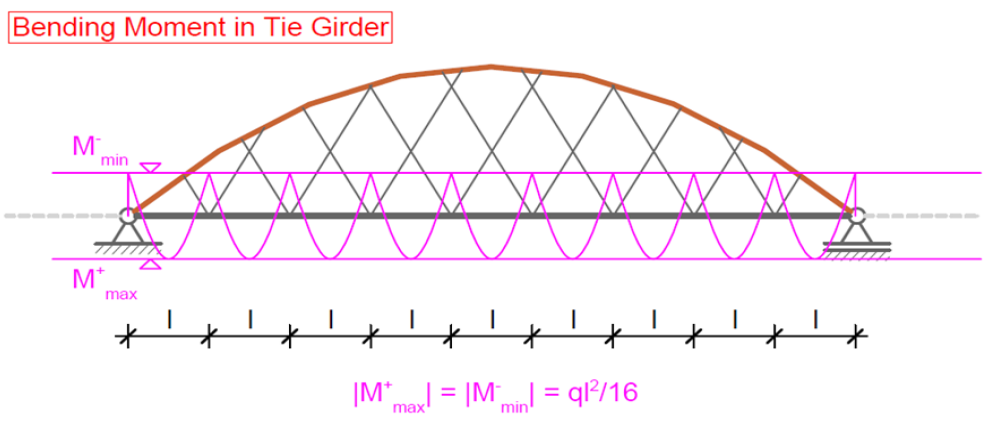
\includegraphics[width=0.73\textwidth]{Pictures/OptimizedBendingMoment.PNG}
    \caption{Determination of the self-equilibrium stress state}
    \label{fig:Cavegn3}
\end{subfigure}%
\begin{subfigure}{.5\textwidth}
    \centering
    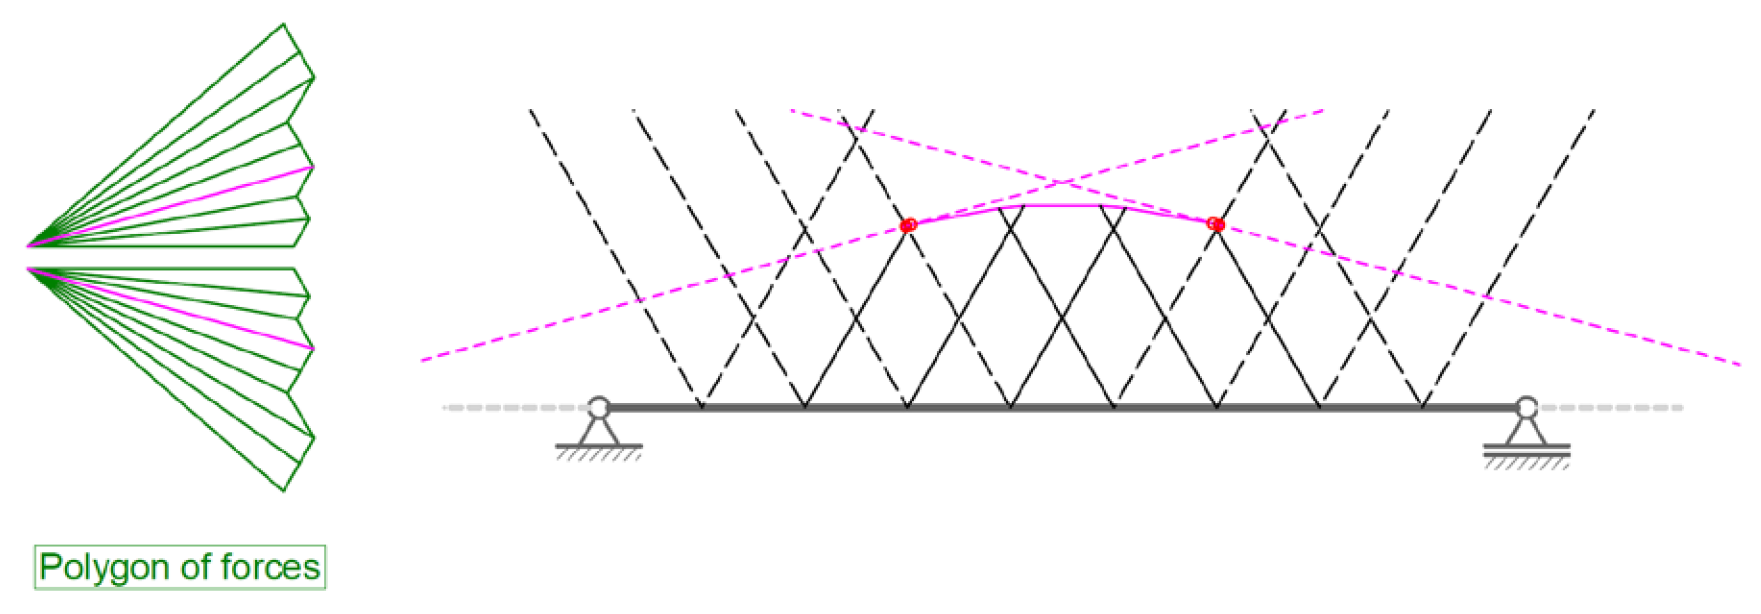
\includegraphics[width=0.9\textwidth]{Pictures/GraphicalThrustLineConstruction.PNG}
    \caption{Graphical construction of the arch shape}
    \label{fig:Cavegn4}
\end{subfigure}
\caption{Optimisation steps \cite{Cavegn}}
\label{fig:Cavegn34}
\end{figure}
It was found, that the obtained arch geometries generally do not correspond to the circular or the parabolic shape. Sometimes they even lie outside of the two traditionally used shapes. By approximating the obtained shape with a quartic function, an analytical expression close to the thrust line was found, deviating by a maximum of 2\% of its height for most arrangements. Further, it was seen that flat angles of inclination lead to thrust lines that are more inclined near the bearing. Ultimately, the impacts under the unilateral live load combinations were used to estimate the costs of the generated structure in a comparative study. The final design of the Blennerhassett Island Bridge was taken as a reference and its cost was estimated using unit prices and the quantities specified in the design drawings. The cost of each component in the investigated designs was estimated proportionally to the respective elastic stresses. A flatter hanger inclination turned out to reduce the bending moment in the tie and the arch, whereas the maximum hanger forces increased. The estimated costs of the bridge were reduced the most by decreases of inclinations and high initial inclinations. The cost function is thereby minimised by up to 12\%. However also other patterns, e.g. with constant inclination, performed well if the arch geometry is adapted to the thrust line.


\section{Summary} \label{sec:rev_sum}
Along with the increase in popularity of network tied-arch bridges, researchers have investigated its manifold aspects. Starting from the hanger forces, which were aimed to be uniform and safe from unloading, the behaviour under fatigue loading and cable loss has been studied. As each of these aspects necessitates a detailed consideration, not one integral design optimisation has been conducted for a network tied-arch bridge. On top of that, the findings of these investigations favour divergent design parameters and there are varying boundary conditions, such as the live to dead load ratio, which complicate the formulation of general guidelines. In this challenging environment, it is tempting to combine the objectives into a single score, be it from the results of a parametric study or as an objective function for an optimisation method. However, both Teich and Belevicius have exemplified, that this approach does not solve the challenges, it only obfuscates the impact of the design variables on the structural behaviour. The lack of knowledge about this bridge type is still too big for the use of advanced optimisation methods to yield a suitable design. While focusing on the costs of the structural components helps putting different aspects into perspective, it should be remembered that the cost of labour outweigh material and fabrication costs. Ultimately, Cavegn pointed out, that key design considerations, such as the self-equilibrium stress state and the arch shape, have only been addressed in an unsatisfying manner. 


%Further it was pointed out early by \cite{Geissler} that only with a detailed structural model, including accurately modelled knuckles, reliable estimations of the hanger forces can be made.






%\section{Hanger arrangements}
%\paragraph*{Hanger unloading}
%Later, he proposed an arrangement with constant distances between the hanger connection points in the middle of the tie, as shown in \autoref{fig:Tveit}. While the nodes on the arch are spaced equidistantly, the connection points on the tie are constructed with the help of an inclined ellipse and an abscissa and an ordinate depending on the parameters $p_1$ and $p_2$. To determine the points on the tie, linearly spaced vertical lines are drawn to the ellipse. The locations of the nodes on the tie are then determined from the ordinate values of the intersection points.\\
%\begin{figure}[H]
%\centering
%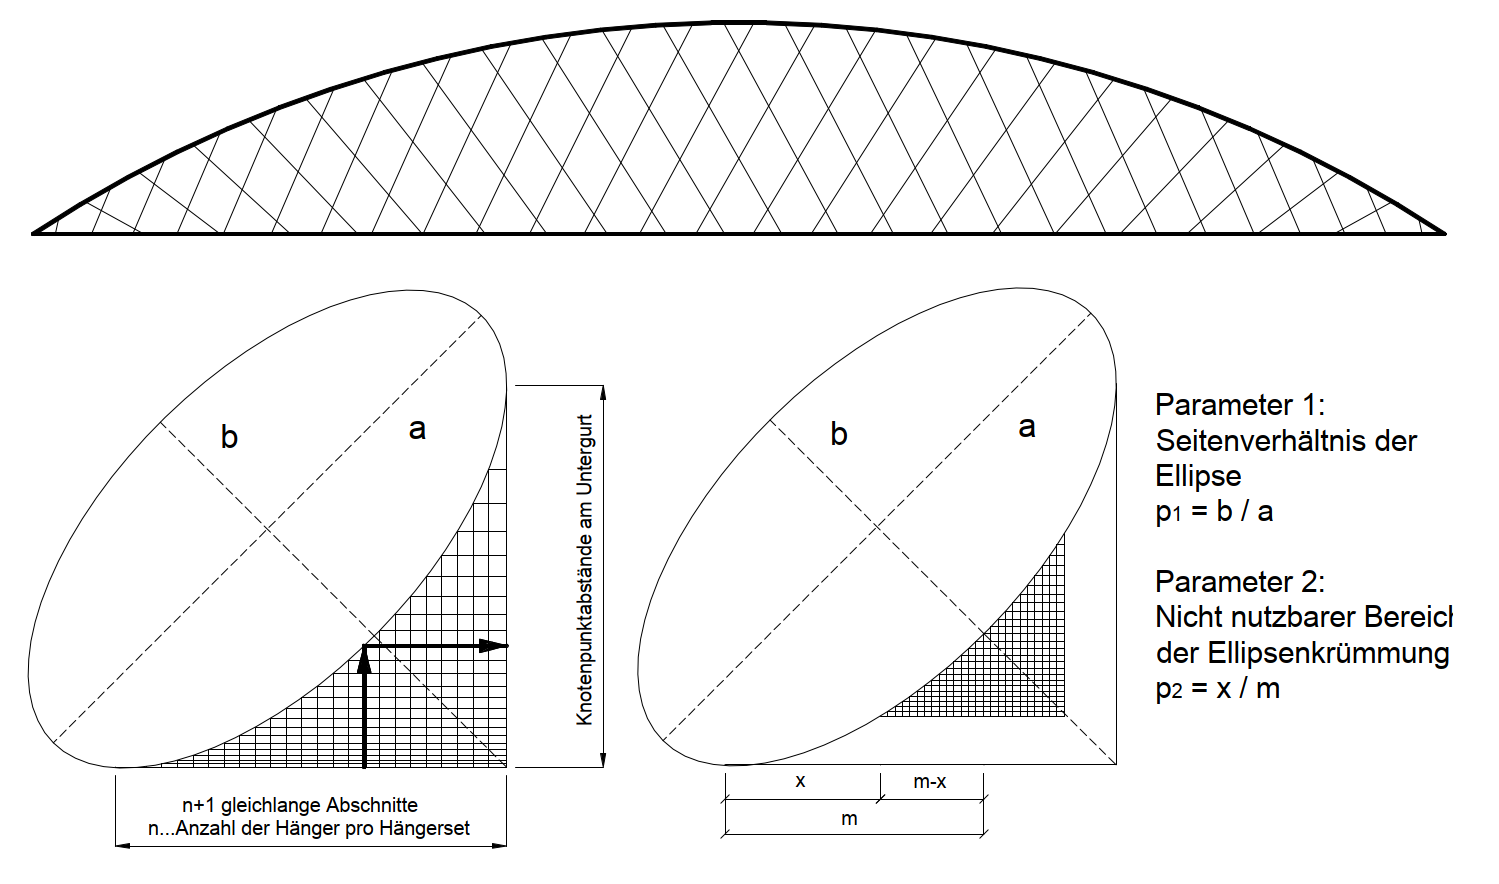
\includegraphics[width=0.7\textwidth]{Pictures/ArrangementTveit.PNG}
%\caption{Arrangement with constant distances in the middle of the tie (adopted from \cite{Teich}).}
%\label{fig:Tveit}
%\end{figure}

%In \cite{Tan} a pedestrian bridge with a sparse hanger arrangement was investigated using an evolutionary optimisation procedure. Each hanger is arranged independently of an overall arrangement. It was found that an arrangement approximately consisting of two separate patterns reduced the internal forces in the arch and the tie the most. Near the knuckles vertical hangers and in the span approximately parallel hangers resulted as shown in \autoref{fig:Tan}.
%\begin{figure}[H]
%\centering
%\begin{subfigure}{0.5\textwidth}
%    \centering
%    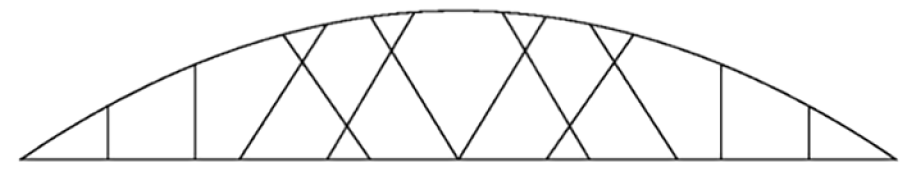
\includegraphics[width=0.9\textwidth]{Pictures/Tan 1.PNG}
%\end{subfigure}%
%\begin{subfigure}{.5\textwidth}
%    \centering
%    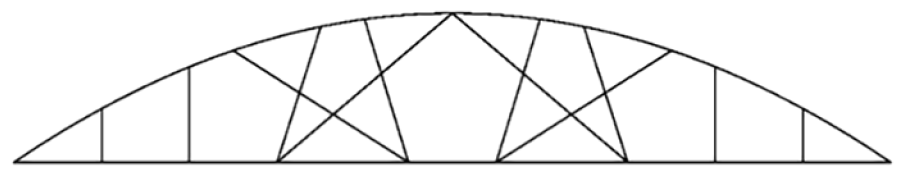
\includegraphics[width=0.9\textwidth]{Pictures/Tan 2.PNG}
%\end{subfigure}
%\caption{Optimal sparse hanger arrangements (adopted from %\cite{Tan}).}
%\label{fig:Tan}
%\end{figure}

%\paragraph*{I don't know}
%In the new millennium, Tveit supervised multiple Master Theses aiming to optimize the design of network tied-arch bridges. In \cite{BrunnSchanack} [nochmals lesen was da genau gemacht wurde]. They developed the radial arrangement aiming to have a pattern which optimally complies with a circular arch. In the radial arrangement, the hangers are equally spaced on the arch and two following hangers cross each other symmetrically to the radius as shown in \autoref{fig:Brunn}. It was the intention, that if the hanger forces are uniform, the thrust line also approximately corresponds to a circle, resulting in an efficient use of the arch. In the literature, this arrangement is either described by the angle $\alpha$ between the arch and the hanger or by the angle $\beta$ between the hangers and the radius at the first intersection point.

%\begin{figure}[H]
%\centering
%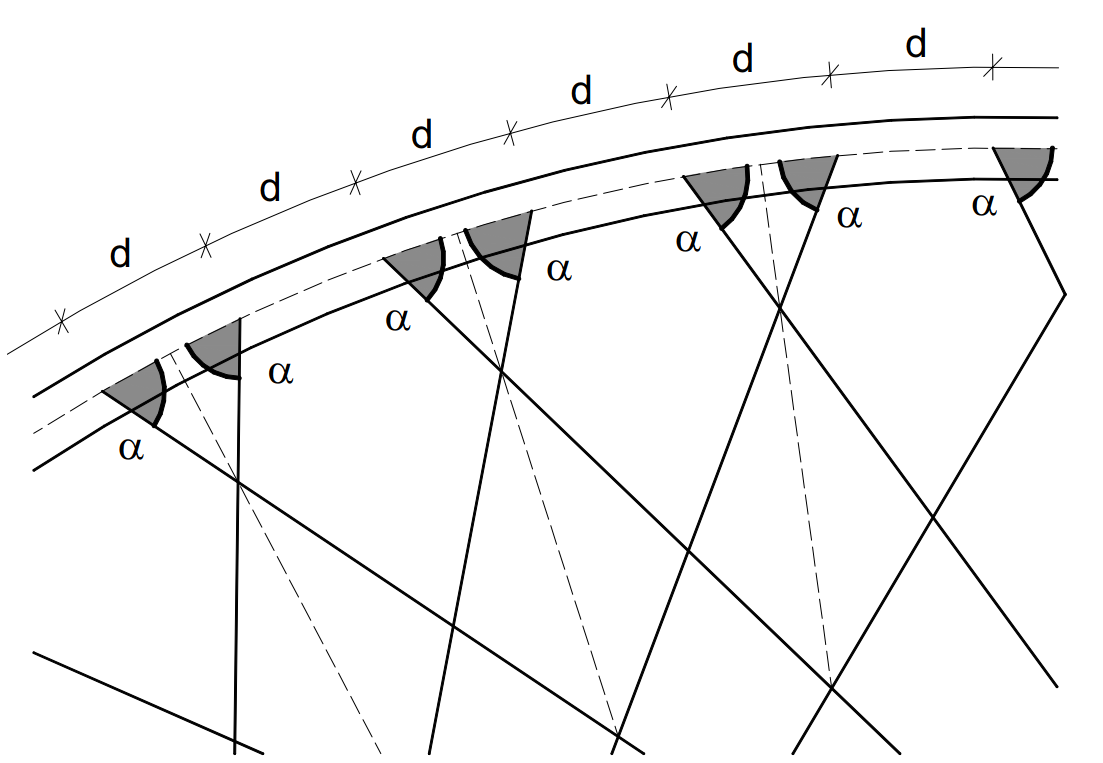
\includegraphics[width=0.4\textwidth]{Pictures/RadialArrangement.PNG}
%\caption{Radial hanger arrangement (adopted from \cite{BrunnSchanack2}).}
%\label{fig:Brunn}
%\end{figure}

%Both of the authors continued their work in the field of network tied-arch bridges and conclude their findings in \cite{BrunnSchanack2}. Besides the bending moments and the maximum hanger forces, also the variation of hanger forces, which are relevant for fatigue, and the elastic embedding of the arch is focused on. These objectives are evaluated manually/arbitrarily. In a comparison of the different hanger patterns, it is concluded that parallel hangers are disadvantageous concerning the bending moments in the arch as the hanger forces vary strongly. Angles of inclination between $55\degree$ and $60\degree$ give the best results. For the constant change of inclination arrangement the middle hanger was recommended to be inclined in the similar range from $56\degree$ to $60\degree$. Further, the change of inclination between two following hangers should lead to an inclination of up to $80\degree$ in the steepest hangers. The radial arrangement was considered optimal, especially for the small corresponding variation of maximum hanger forces and uniform embedding of the arch. The angle between the hangers and the arch are recommended to be between $55\degree$ and $60\degree$. Interestingly, the optimal solutions for each hanger arrangement feature a middle hanger with an inclination of $55\degree$ to $60\degree$. Further, it is recommended that the hanger spacing on the arch lies between \SI{2.5}{m} and \SI{4}{m}.


\cleardoublepage

\chapter{Methods}\label{sec:methods}
In this chapter, the methods for investigating a bridge design, verifying its structural safety and estimating its cost are introduced. In Section \ref{sec:met_ref} the Blennerhassett Island Bridge, as well as other reference bridges, are presented.
Section \ref{sec:met_str} introduces the structural model and briefly assesses its underlying assumptions. Further, an overview of the investigated load cases is given in Section \ref{sec:met_loads}. The determination of the self-equilibrium stress state is of critical importance. The designer can freely assign it to the structure, contrary to the load cases, whose effects are determined by the elastic response of the structure. Section \ref{sec:met_seq} describes different methods to obtain this state which also includes the choice of the arch shape. The limit states for the design criteria as well as the corresponding verifications are specified in Section \ref{sec:met_ver}, combining the self-equilibrium stress state with the factored load cases. Based on these verifications, the cost of an investigated design is estimated according to Section \ref{sec:met_cost}. The methods presented in this chapter are exemplified by the final design of the Blennerhassett Island Bridge based on the design drawings.

\section{Reference bridges} \label{sec:met_ref}

\newpage
\section{Structural model} \label{sec:met_str}
A defining feature of the Blennerhassett Island Bridge is the floating deck. It is supported only at the 13 floor beams and acts almost structurally independent and resembles a bridge by itself. Compared to a composite deck, it causes a certain inefficiency in material use and the additional arrangement of many bearings. On the other hand, it allows for a replacement of the deck in the future and it simplifies the investigation of the flow of forces. It carries the loads over a span of 20 meters to the adjacent floor beams. There, the forces are mainly carried by the respective hanger pair and partially by the tie girder. This feature allows for a separation of the behaviour of the remaining network arch from the deck. As it is not the objective of this Thesis to investigate and optimise the deck system it is not further considered. The structural model of the network tied-arch bridge is therefore composed of the tie, the arch and the hangers. According to Smit, the behaviour of the two planes of the arch can be considered decoupled from each other \cite{Smit}. Therefore, the behaviour of the arch is analysed in a single arch plane. In the design drawings, the structure is divided into segments for the arch and the tie. Each of these segments is verified independently in the design verifications. This segmentation, which is shown along with the bridge in Figures \ref{fig:Blennerhassett2_a} and \ref{fig:fig:Blennerhassett2_b}, is also used for the analysis in this Thesis.

\begin{figure}[H]
\centering
\begin{subfigure}{0.5\textwidth}
    \centering
    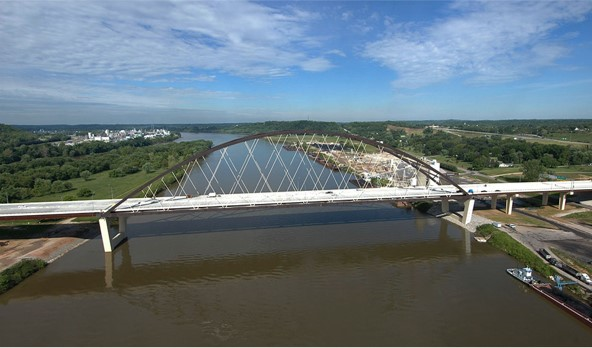
\includegraphics[width=0.9\textwidth]{overleaf/Pictures/Blennerhassett_2.jpg}
    \caption{Built structure}
    \label{fig:Blennerhassett2_a}
\end{subfigure}%
\begin{subfigure}{.5\textwidth}
    \centering
    \vspace*{0.67cm}
    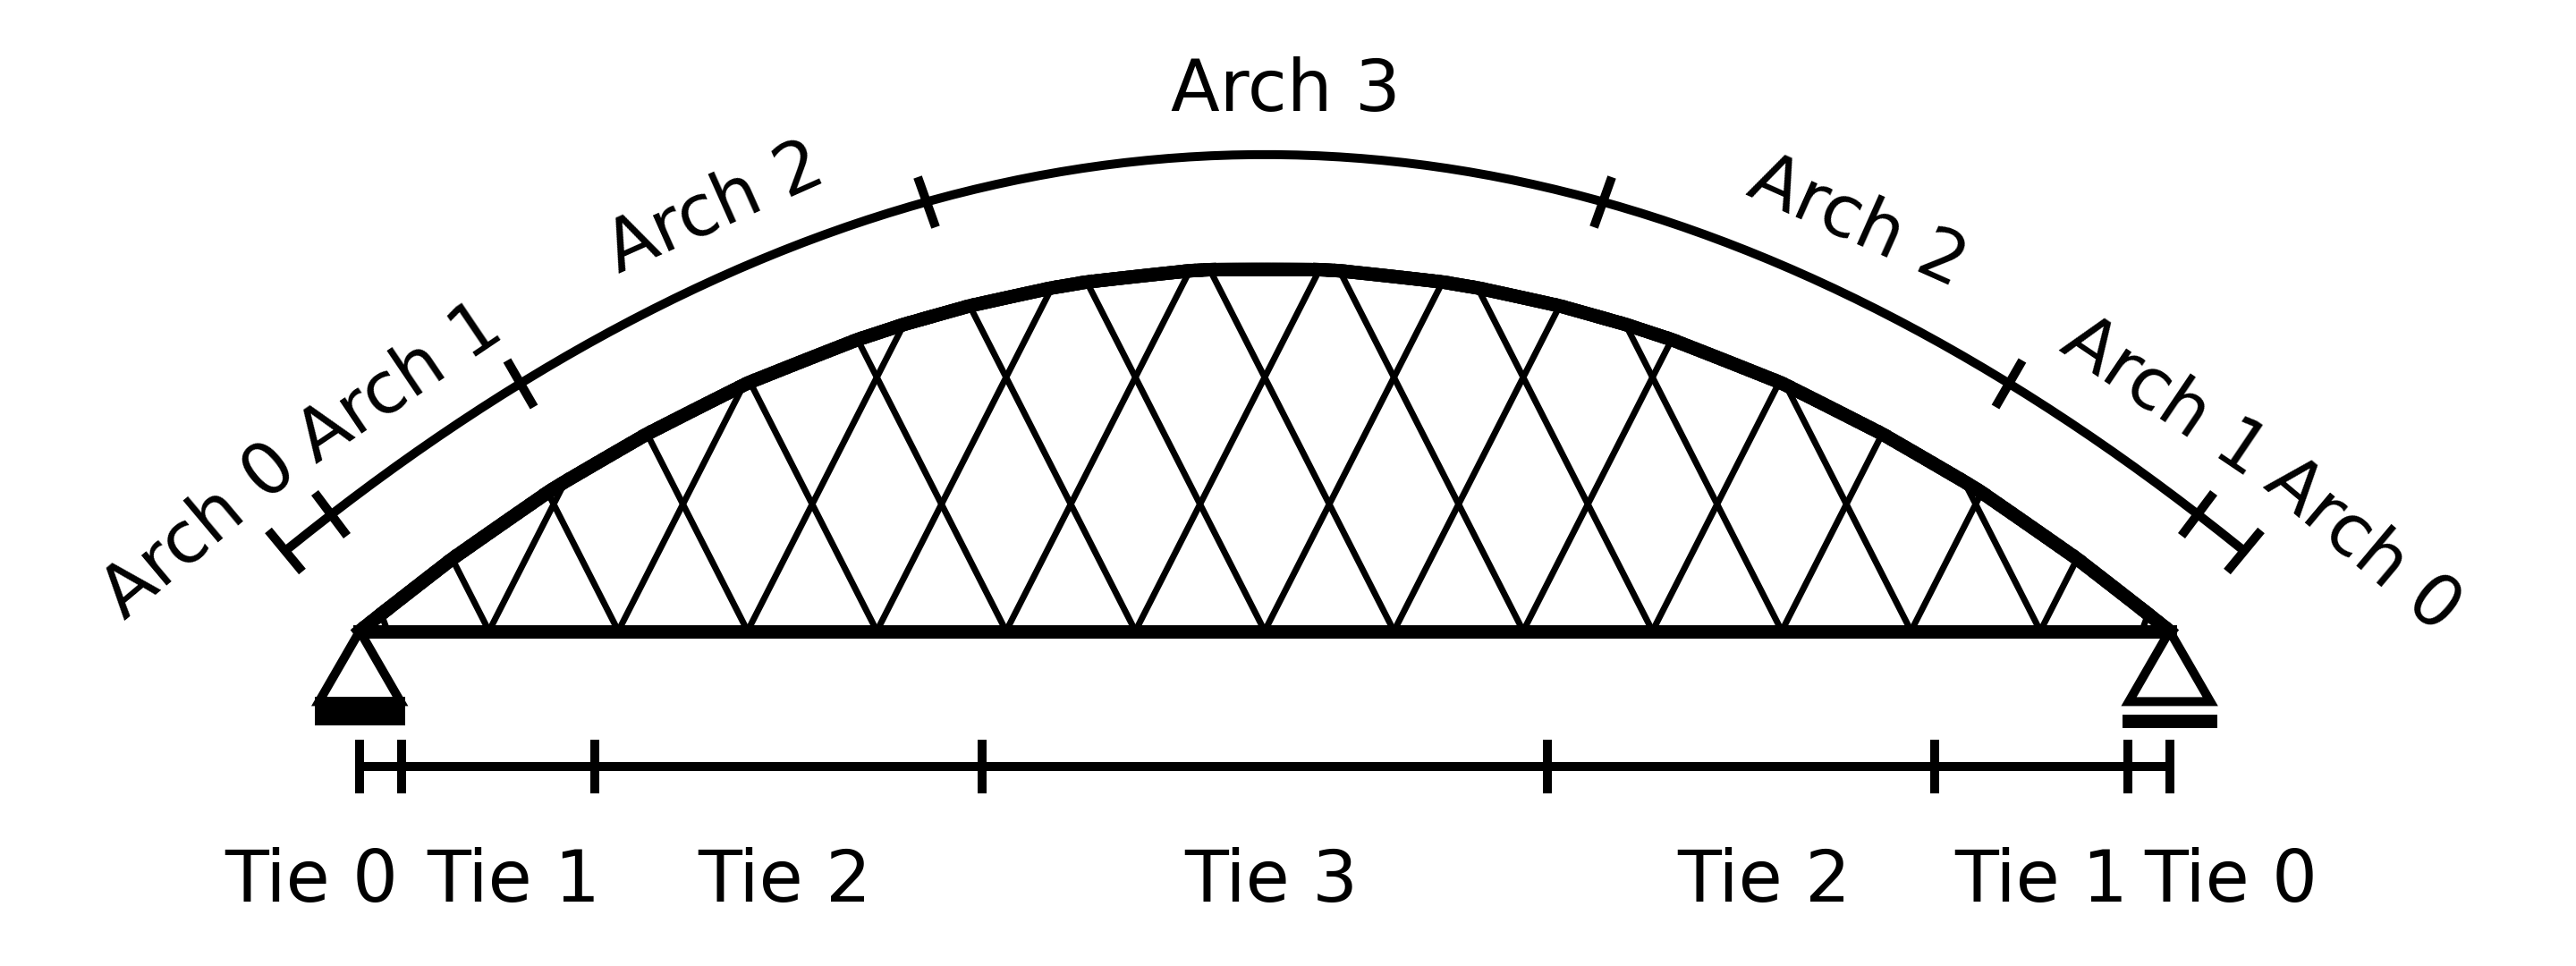
\includegraphics[width=0.9\textwidth]{illustrations/figures/segments.png}
    \vspace*{0.67cm}
    \caption{Structural model and segments}
    \label{fig:fig:Blennerhassett2_b}
\end{subfigure}
\caption{Blennerhassett Island Bridge}
\label{fig:Blennerhassett2}
\end{figure}

Both the arch and the tie girder feature are a box cross-section with a width of \SI{1.2}{m}. The one of the arch is \SI{1.7}{m} high and offers similar bending resistances around both axes. Additionally, it is reinforced by a web stiffener to prevent local buckling. The cross-section of the tie girder is \SI{2.2}{m} high and offers more resistance for longitudinal than transverse bending moments. Both the arch rib and the tie girder feature a stronger cross-section in the knuckle region, where the highest internal force effects are expected. The segments Arch 0 and Tie 0 form the knuckle and are assigned the strongest cross-sections, with resistances about 50\% higher than in the field. They are not subject to the optimisation in this Thesis as they cannot accurately be dimensioned as beam elements. Also the next segments Arch 1 and Tie 1 have a slightly enhanced cross-section with thicker plates. The remaining segments in the field feature identical cross-sections for the tie girder and the arch rib respectively. They are considered the characteristic cross-sections and are shown in Figures \ref{fig:cs_arch} and \ref{fig:cs_tie}. All cables have identical cross-sections with 29 high-strength strands of \SI{140}{mm^2}. The respective lengths range from \SI{11}{m} to \SI{59}{m}. The corresponding cross-section including its tube is shown in Figure \ref{fig:cs_cable}. The most important properties are specified in Table \ref{tab:cs_properties}. More detailed specifications on the cross-sections are found in the Appendix \ref{app:cross_sections}.

\begin{figure}[H]
\centering
\begin{subfigure}{0.33\textwidth}
    \centering
    \vspace*{0.68cm}
    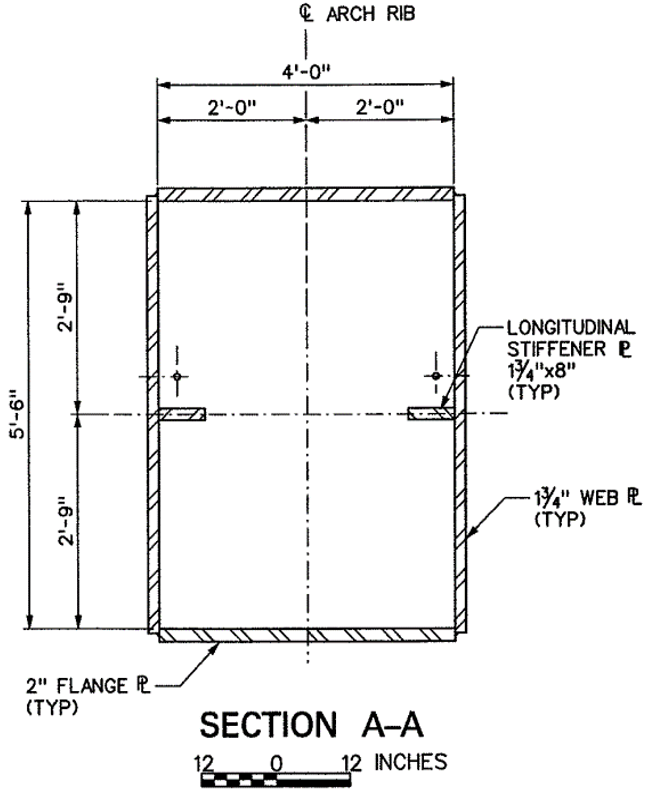
\includegraphics[width=0.8\textwidth]{overleaf/Appendix/Pictures/arch_3.PNG}
    \vspace*{0.68cm}
    \caption{Arch rib}
    \label{fig:cs_arch}
\end{subfigure}%
\begin{subfigure}{.33\textwidth}
    \centering
    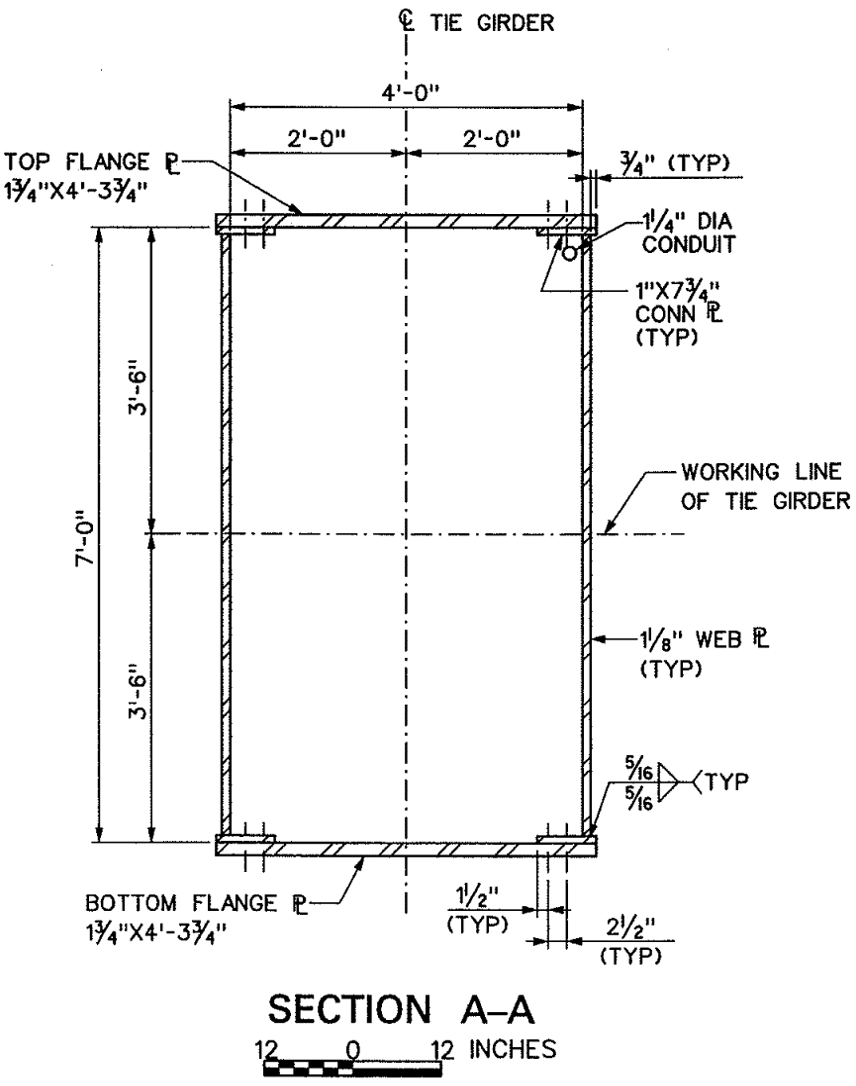
\includegraphics[width=\textwidth]{overleaf/Appendix/Pictures/tie_3.PNG}
    \caption{Tie girder}
    \label{fig:cs_tie}
\end{subfigure}%
\begin{subfigure}{.33\textwidth}
    \centering
    \vspace*{1.35cm}
    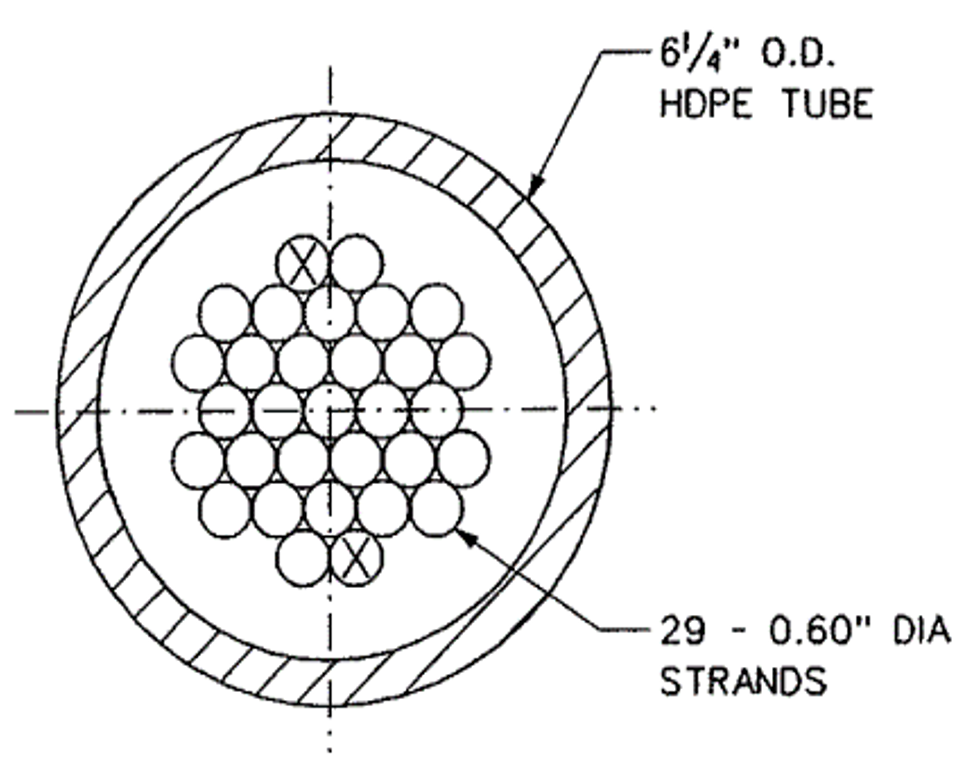
\includegraphics[width=0.9\textwidth]{overleaf/Appendix/Pictures/cable_3.PNG}
    \vspace*{1.35cm}
    \caption{Cable}
    \label{fig:cs_cable}
\end{subfigure}\caption{Cross-sections in the field}
\label{fig:cross_sections}
\end{figure}

\begin{table}[H]
    \centering
    \caption{Properties of the field cross-sections}
    \label{tab:cs_properties}
    \begin{tabular}{lccccc}
    \toprule
    Cross-section & $EA$ & $EI$ & $N_{Rd}$ & $M_{Rd,z}$ & $M_{Rd,y}$ \\
                  & [\SI{}{GN}]   & [\SI{}{GNm^2}]   & [\SI{}{MN}]  & [\SI{}{MNm}]  & [\SI{}{MNm}] \\ \midrule
    Arch 2 \& Arch 3 & 61.8 & 28.1 & 82.3 & 50.0 & 42.7 \\
    Tie 2 \& Tie 3  & 53.7 & 42.8 & 100.5 & 76.2 & 45.8 \\
    Cables        & 0.8 &  - & 6.8 & - & - \\ \bottomrule
    \end{tabular}
\end{table}

Considering their slenderness, the arch and the tie can be accurately modelled as beam elements. On the other hand, secondary effects cannot always be neglected for the hangers because of their low bending stiffness. However, a brief investigation, given in Appendix \ref{Appendix_A_Hangers}, shows that above \SI{100}{MPa} these effects are irrelevant. Therefore, the hangers are modelled as beams with rotational end releases and their self-weight is neglected. Additionally, two web plates connecting the tie girder and the arch rib in the knuckle region are arranged to obtain a more accurate representation of this detail. Each web plate has a cross section of \SI{6.3}{cm} x \SI{1.07}{m} and is arranged \SI{4.1}{m} for the idealised node at an angle of 80\degree. The web plates are illustrated in Figure \ref{fig:knuckle_region}.



\begin{figure}[H]
    \centering
    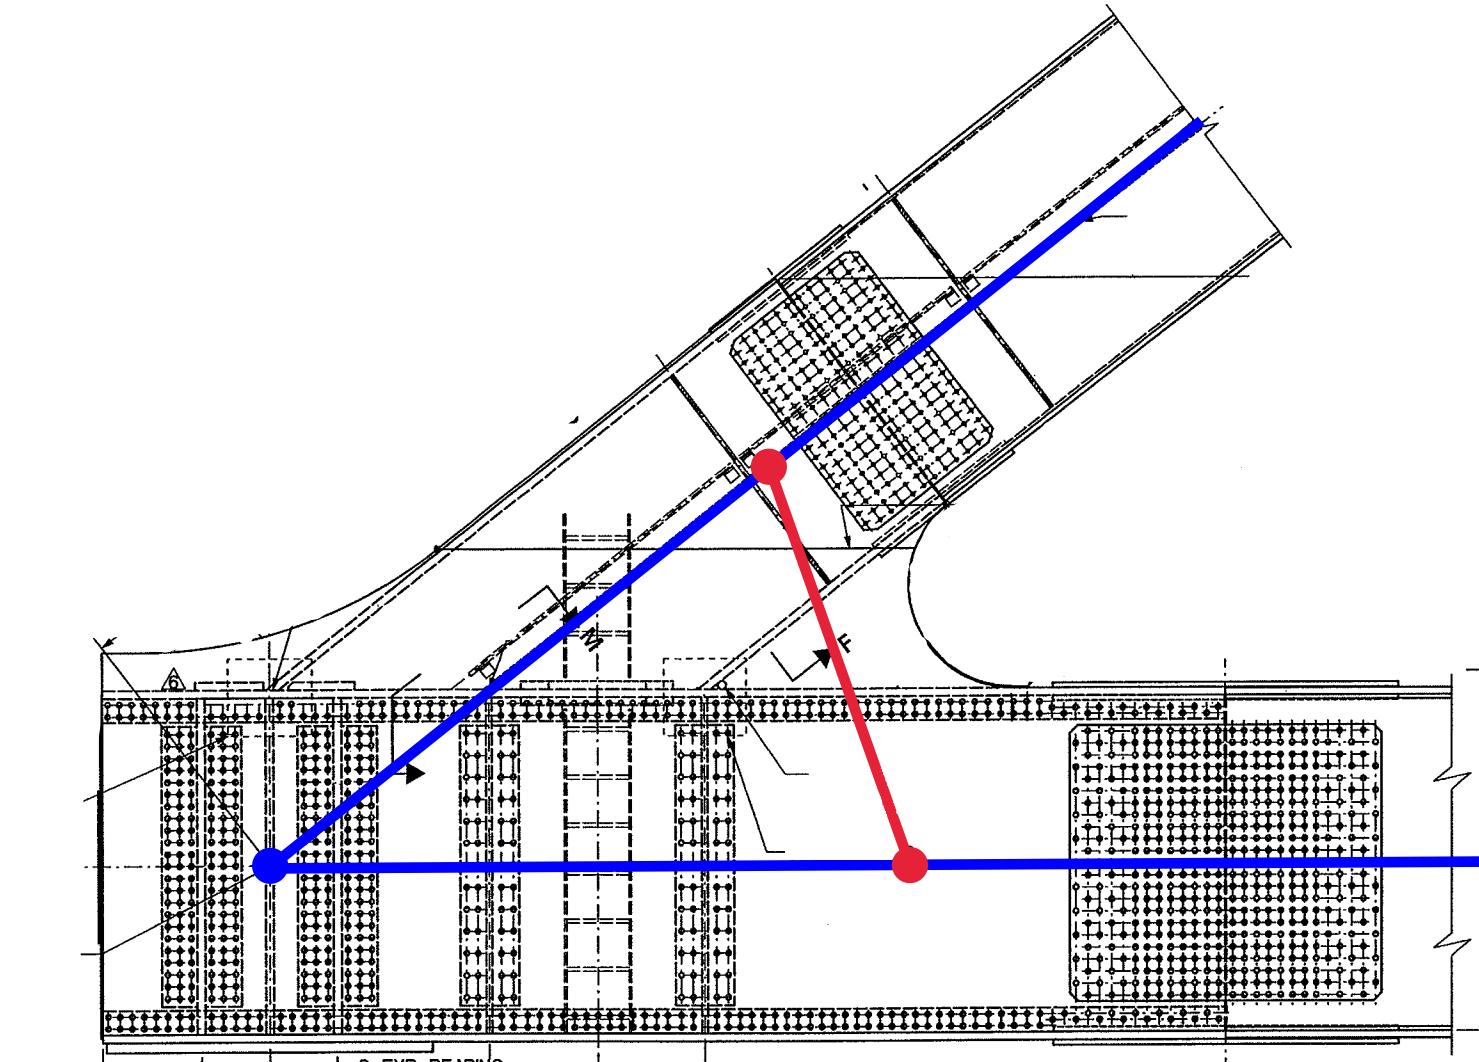
\includegraphics[width=0.5\textwidth]{overleaf/Pictures/Knuckle region.png}
    \caption{Plan and structural model of the knuckle region}
    \label{fig:knuckle_region}
\end{figure}

The structure is analysed in the framework of two-dimensional and linear elastic beam statics. Therefor, a python package written by the author in an earlier project is used. It is verified with the Sofistik model of a parallel Master Thesis in Appendix \ref{app:model_verification}. To judge the dependency of the resulting internal force effects on the described modelling, the structure is first analysed using different simplified models. In the first simplistic model, the field cross-sections are used everywhere and also no web member is considered. In a second model, the previously described web plated are introduced. Additionally, the actual cross-sections are assigned to the arch and the tie in a third model. The elastic effects under dead loads are compared in Figure \ref{fig:model_comparison}.

\begin{figure}[H]
    \centering
    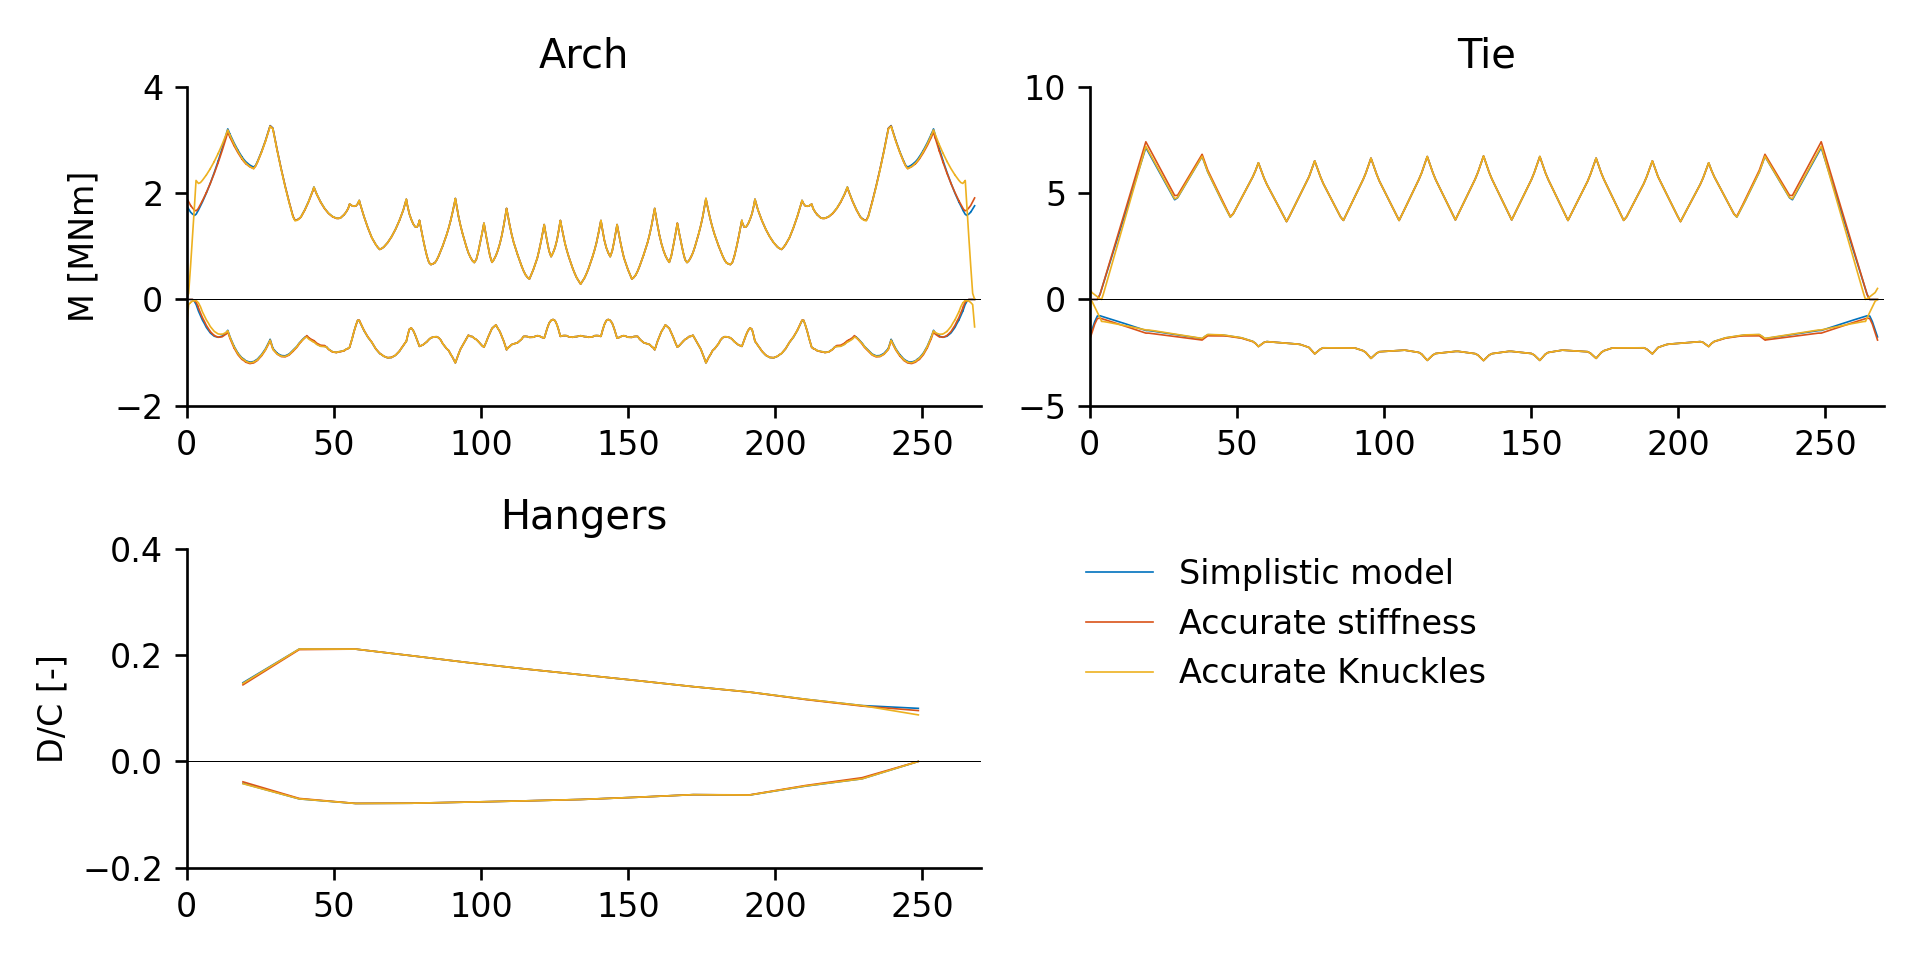
\includegraphics[width=0.9\textwidth]{calculations/model comparison/live_loading.png}
    \caption{Comparison of the elastic responses under live loading for different models}
    \label{fig:model_comparison}
\end{figure}

[Conclusion]

\newpage
\section{Load cases} \label{sec:met_loads}
The load cases relevant to this investigation are the dead loading (DL), the live loading (LL) and the wind loading (WS). The dead loading is further subdivided into the weight of the structural components and non-structural attachments (DC) and the weight of the future wearing surfaces and utilities (DW).

\subsection{Dead loading}
The dead loads for the Blennerhassett Island Bridge were derived from the estimated bridge quantities of the design drawings. The detailed derivation is given in Appendix \ref{app:weight} and the final results are presented in Table \ref{tab:dead_loads}. The weight of the arch and the tie girder are distributed as a constant load along the respective elements. A particularly detailed weight distribution by assigning more weight to the stronger cross-sections near the knuckle is disregarded for. Also the weight of the lateral arch bracing is distributed along the entire arch for simplicity. The deck weight and its non-structural components make up for the main contribution to the dead loading. The weight of the deck is applied as a concentrated force at the locations of the floor beams. The weight of the hangers and its resulting bending moment is relatively small and neglected to facilitate some of the used optimisation methods. An illustration of all dead loads applied to the structural model is shown in Figure \ref{fig:dead_loads}.

\begin{table}[H]
    \centering
    \caption{Weights of the structural and non-structural components}
    \label{tab:dead_loads}
    \begin{tabular}{lcccc}
        \toprule
        Component & Arch & Tie & Deck & Utilities \\ \midrule
        Weight & \SI{29.8}{kN/m} & \SI{26.4}{kN/m} & \SI{115.3}{kN/m} & \SI{35.1}{kN/m} \\ \bottomrule
    \end{tabular}
\end{table}

\begin{figure}[H]
    \centering
    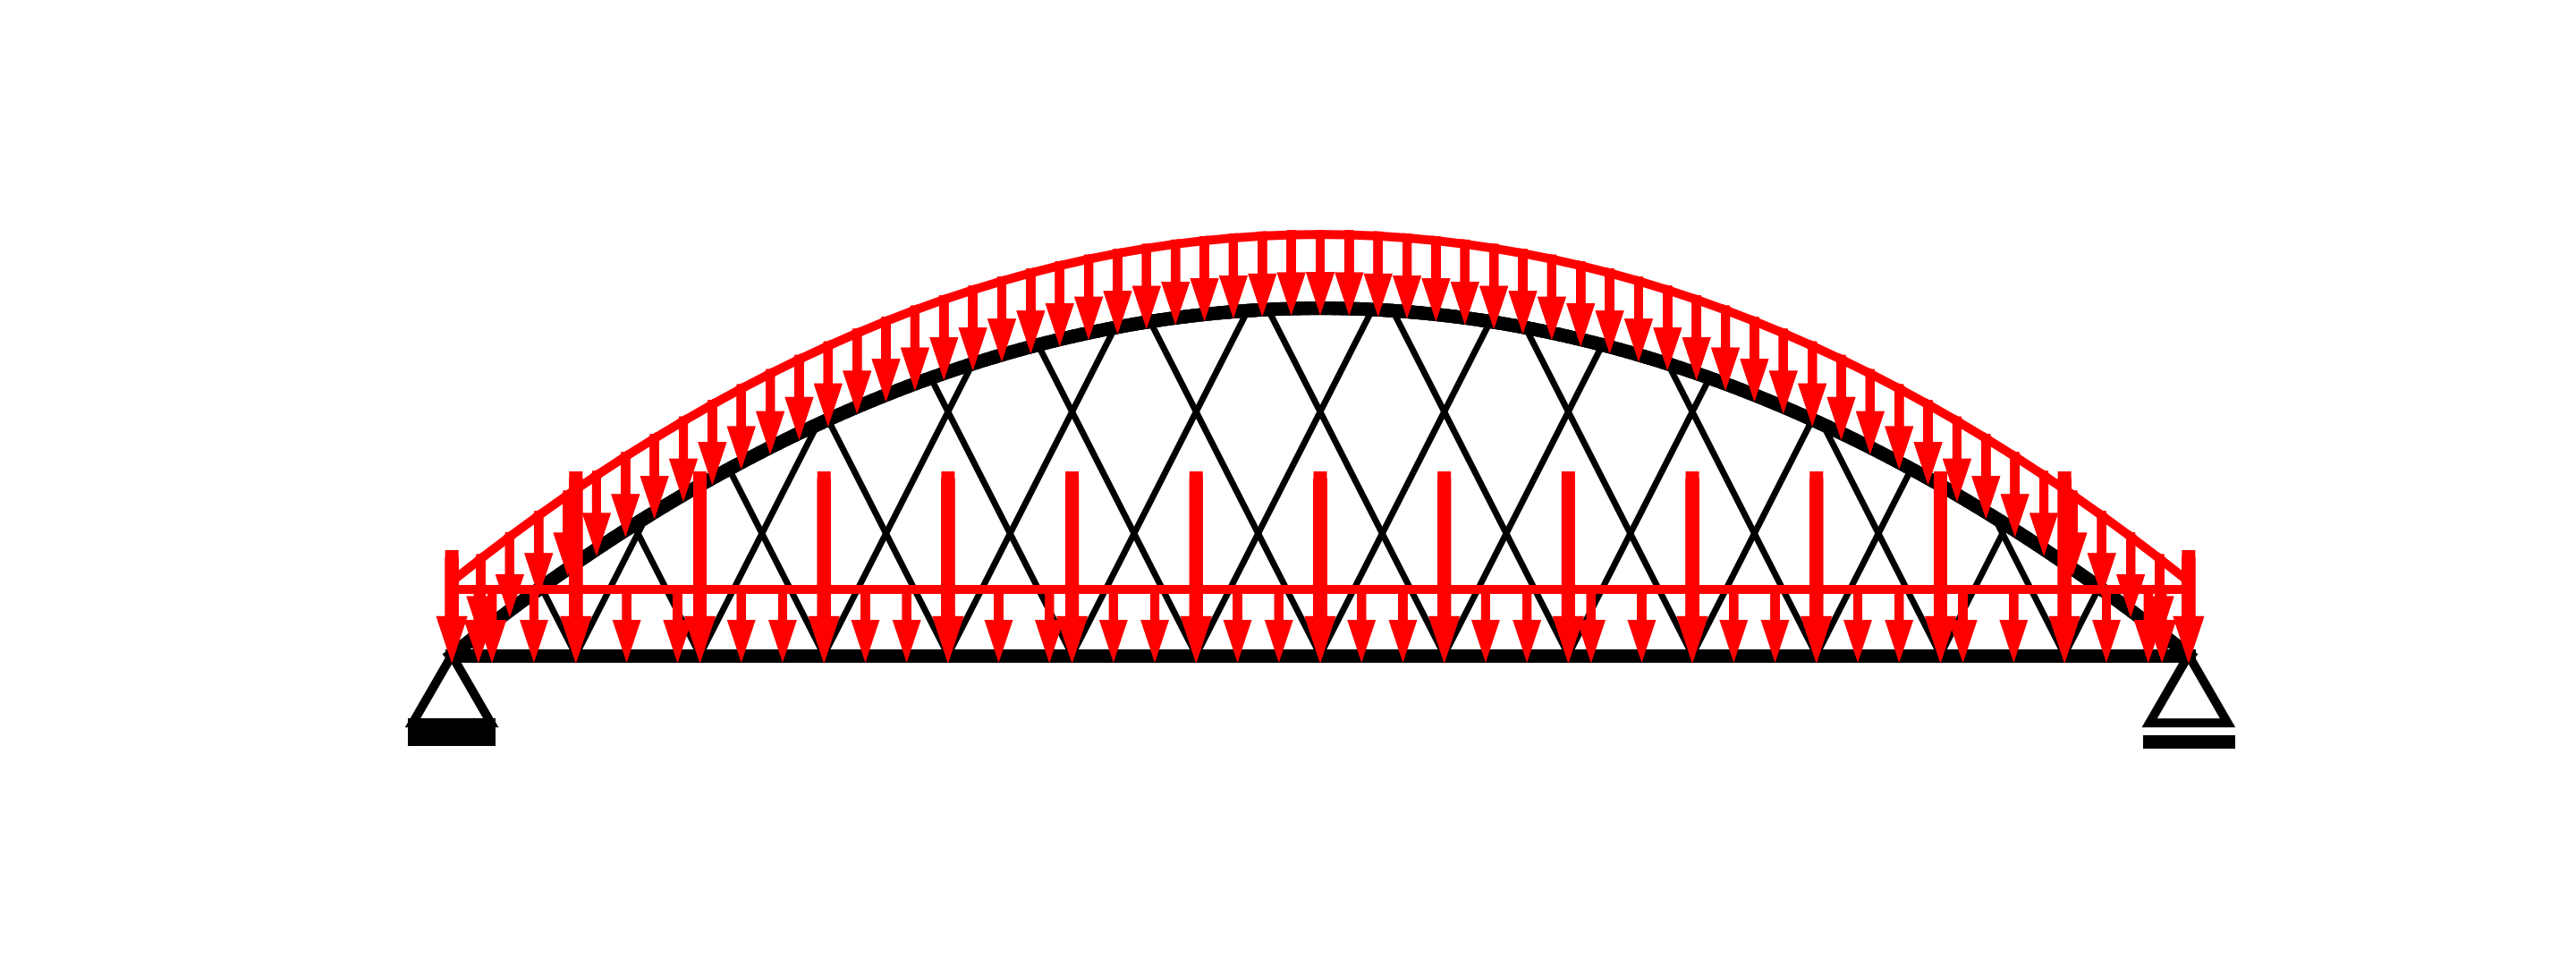
\includegraphics[trim={0 0.8cm 0 0.8cm},clip,
    width=0.8\textwidth]{illustrations/figures/permanent loads.png}
    \caption{Dead loading in the structural model}
    \label{fig:dead_loads}
\end{figure}

\subsection{Live loading} \label{sec:met_loads_live}
The load case of live loading is taken into account according to the AASHTO Bridge Design Specifications (1998) \cite{AASHTO}. It is a combination of two separate components: A lane-wise distributed load is applied along the entire or partial length of the bridge and a concentrated truck load is applied at a single longitudinal point. Both loads are factored by a multiple presence factor (MPF) depending on how many lanes are loaded. In a detailed calculation in Appendix \ref{Appendix_Liveloading}, six loaded lanes were found to cause the highest load in the considered arch plane. This conclusion also applies to the truck loads, which are also applied simultaneously on six lanes. An overview of the design loads is given in Table \ref{tab:live_load_overview}. 

\begin{table}[H]
\centering
\caption{Overview of the live loading}
\label{tab:live_load_overview}
\begin{tabular}{cccccc}
\begin{tabular}[c]{@{}c@{}}Design\\ lane load\end{tabular} & \begin{tabular}[c]{@{}c@{}}Design\\ truck weight\end{tabular} & \begin{tabular}[c]{@{}c@{}}Lane\\ multiplier\end{tabular} & \begin{tabular}[c]{@{}c@{}}Dynamic\\ multiplier\end{tabular} & \begin{tabular}[c]{@{}c@{}}Distributed\\ design load\end{tabular} & \begin{tabular}[c]{@{}c@{}}Concentrated\\ design load\end{tabular} \\ \hline
\SI{9.3}{kN/m} & \SI{325}{kN} & \SI{2.46}{} & \SI{1.33}{} & \SI{23.0}{kN/m} & \SI{1063}{kN}
\end{tabular}
\end{table}


The live loads are applied on the deck, which is not part of the structural model. Therefore, the live loads act as concentrated forces on the floor beams, where the deck is supported, as illustrated in Figures \ref{fig:Live_load_1} for the fully loaded deck. To find the worst arrangement of the live loads, the concentrated forces are applied individually. For each point of interest in the model, the partially distributed lane load and the concentrated truck force are then combined to produce maximum effects. The concentrated force is thereby only applied at one cross-girder exclusively, as shown in Figure \ref{fig:Live_load_2}. 

%It yields a range of possible effects for each point on the structural elements. The resulting ranges for the Blennerhassett Island Bridge are presented in Figure [], where the ranges of the concentrated load and the distributed loads are also shown individually. These results agree well with the effects specified on the design drawings.\bigskip

\begin{figure}[H]
\centering
\begin{subfigure}{0.5\textwidth}
    \centering
    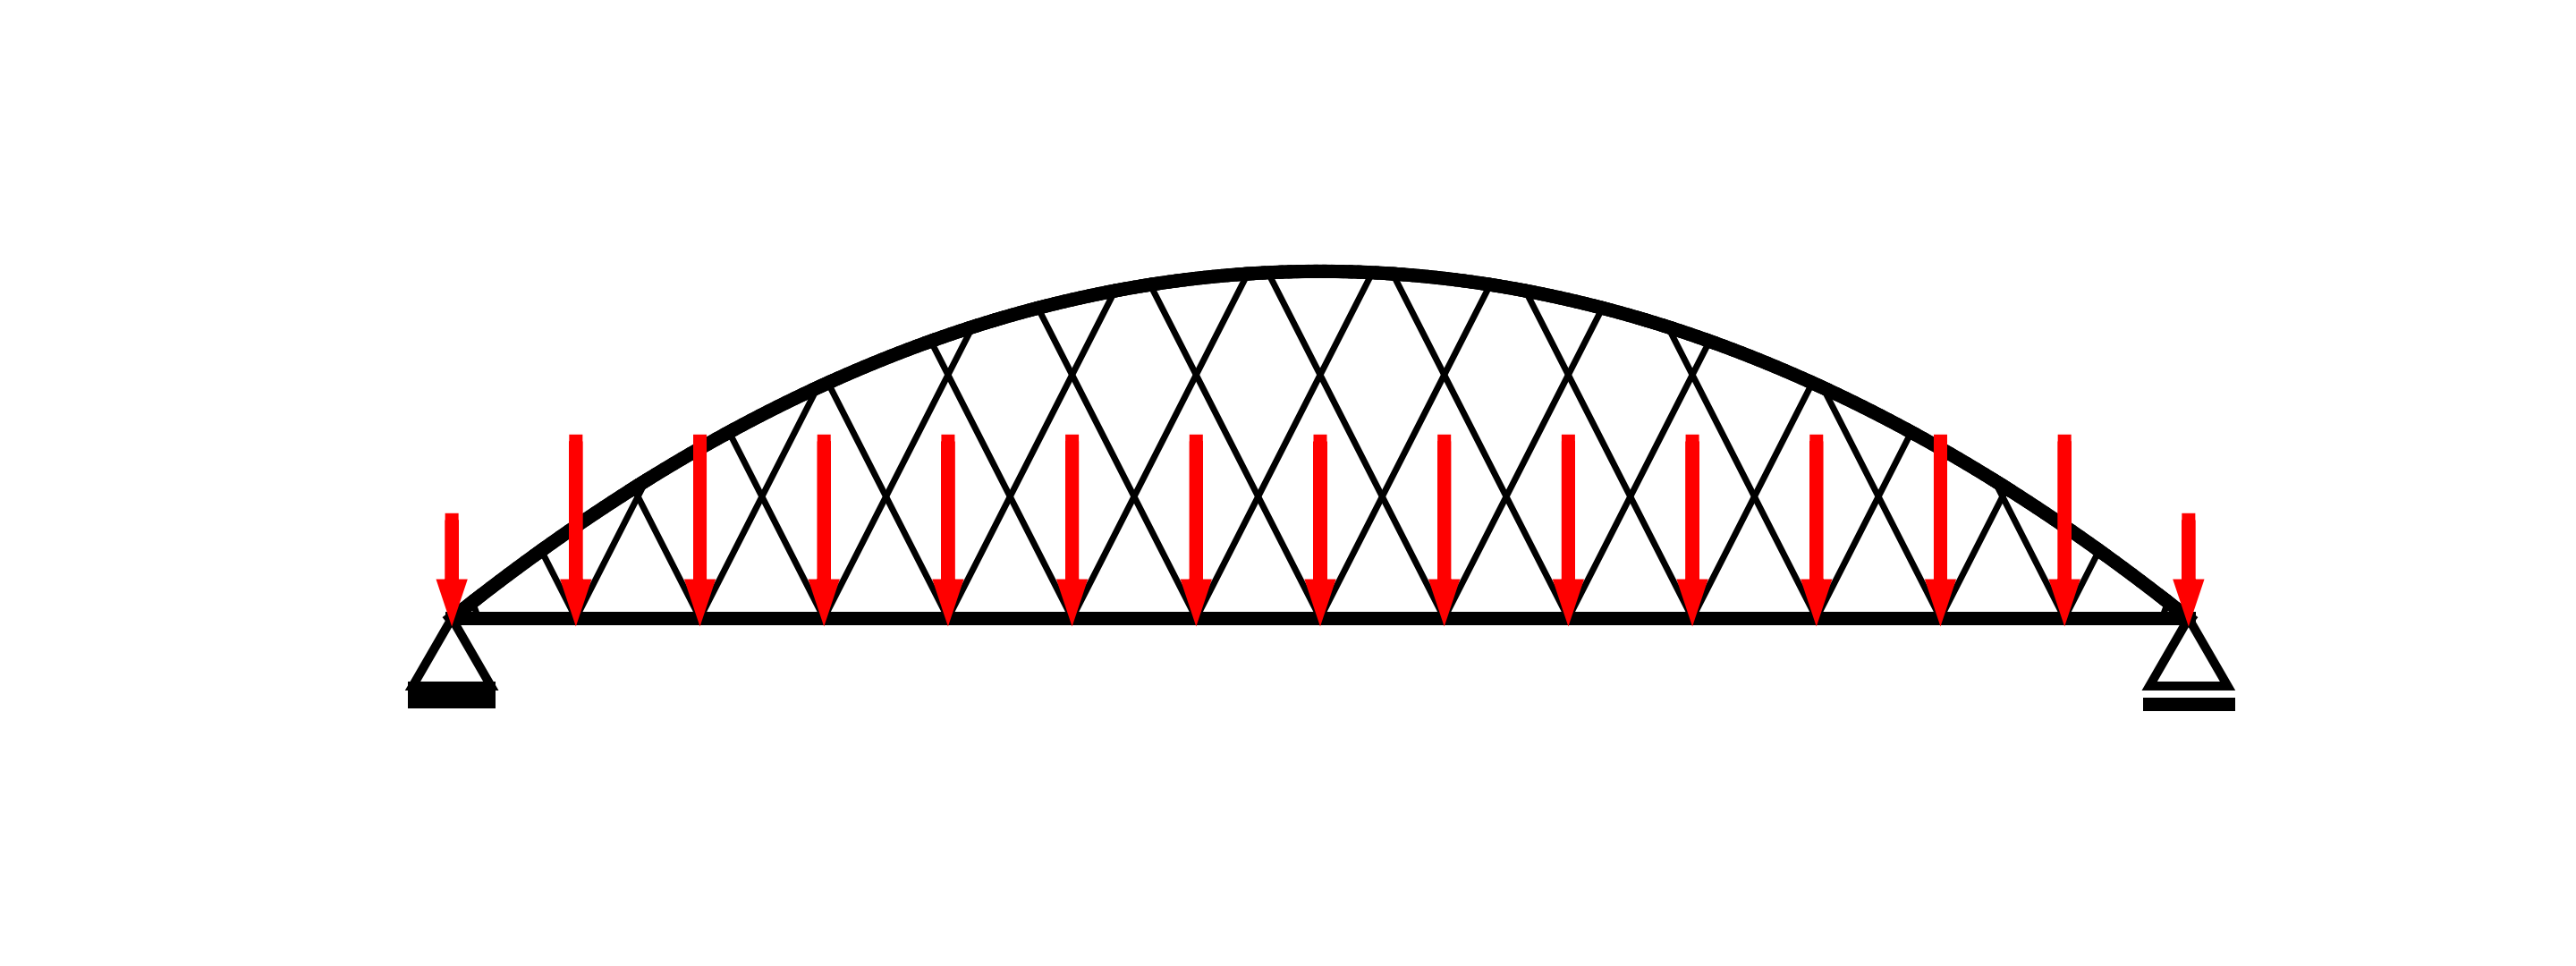
\includegraphics[trim={0 0.8cm 0 0.8cm},clip, width=0.9\textwidth]{illustrations/figures/distributed live loads.png}
    \caption{Distributed live loads}
    \label{fig:Live_load_1}
\end{subfigure}%
\begin{subfigure}{.5\textwidth}
    \centering
    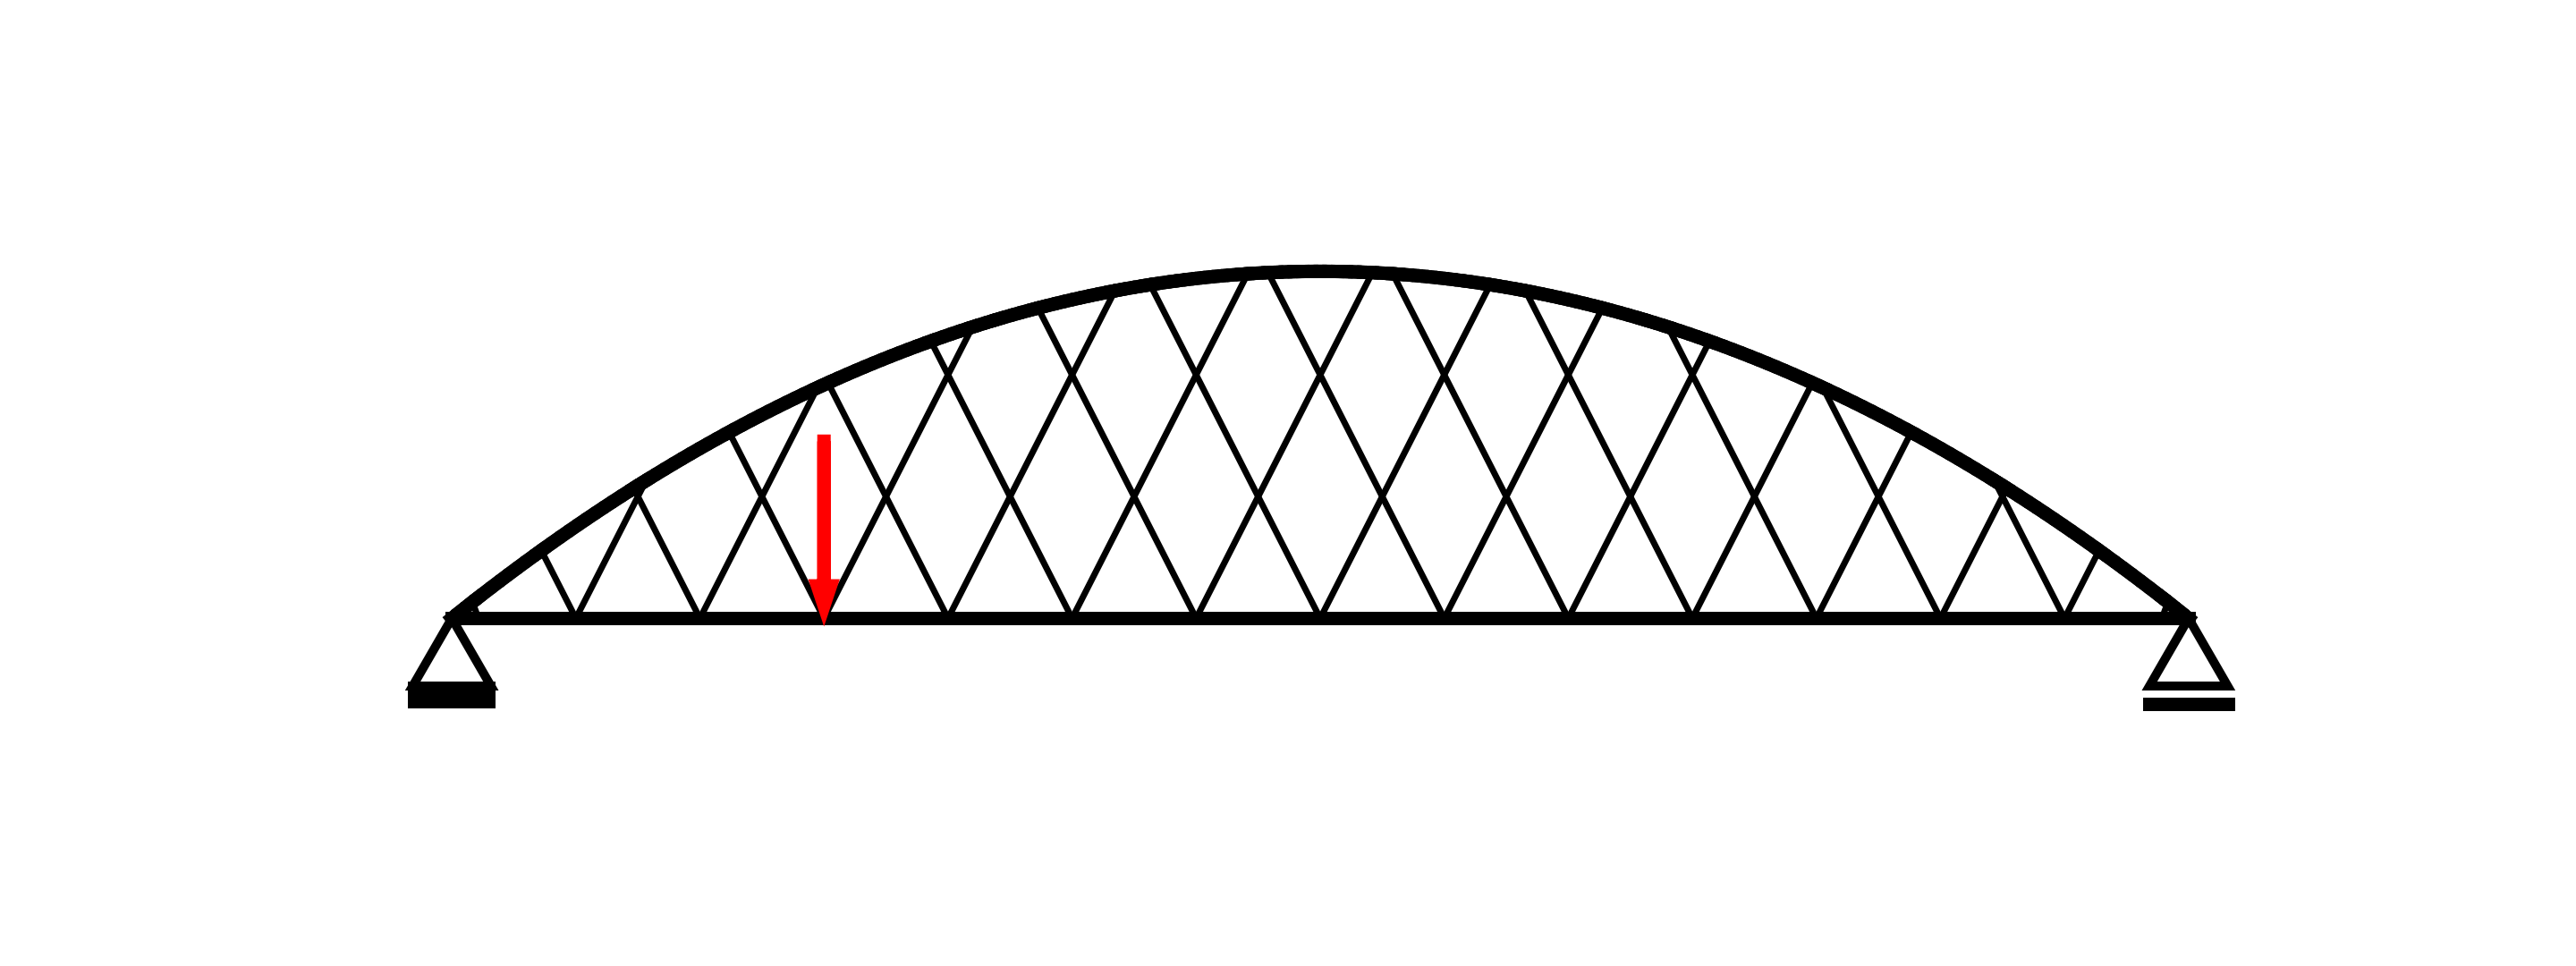
\includegraphics[trim={0 0.8cm 0 0.8cm},clip, width=0.9\textwidth]{illustrations/figures/concentrated live loads.png}
    \caption{Concentrated live loads}
    \label{fig:Live_load_2}
\end{subfigure}
\caption{Live loading in the structural model}
\label{fig:Live_load}
\end{figure}

For the extreme events of cable loss and cable replacement, special circumstances apply to the live loading. For cable loss, it is assumed that only the actually marked lanes are loaded. For cable replacement, one lane is shifted away from the replaced hanger. The determining live load arrangement is also calculated and illustrated in the Appendix \ref{Appendx_A_Live_loading_2}. The resulting loads on the tie are given in Table \ref{tab:live_load_extreme}. For the event of tie fracture, the same live loading as in the ultimate limit states is applied.

\begin{table}[H]
\centering
\caption{Live loads for extreme events}
\label{tab:live_load_extreme}
\begin{tabular}{lcc}
\hline
Extreme event     & Distributed live load & Concentrated live load \\ \hline
Cable loss  & \SI{14.2}{kN/m} & \SI{660}{kN} \\
Cable replacement & \SI{18.8}{kN/m} & \SI{874}{kN} \\ \hline
\end{tabular}
\end{table}


For the fatigue limit state, the loading according to the PTI specifications is used \cite{PTI}. It consists of a single design truck without taking into account the dynamic multiplier. The resulting force, which is derived in the Appendix \ref{Appendx_A_Live_loading_2}, is equal to \SI{296}{kN}.



\subsection{Wind loading}
The load case of wind loading is not calculated in this investigation as the loads are particular to a specific design and require a 3-dimensional model and a very detailed investigation. However, the effects specified on the design drawings, shown in the Appendix \ref{app:design_verifications}, are taken to allow for an integral design verification. The respective characteristic internal force effects under wind loading are shown for each segment in Table \ref{tab:effects_wind_load}.

\begin{table}[H] 
\caption{Effects of wind loading per segment}
\label{tab:effects_wind_load}
\centering
\begin{tabular}{lccc}
\hline
Segment & Normal force & Moment-y & Moment-z \\
 & [MN]   & [MNm] & [MNm] \\ \hline
Arch 1 & -7.8 & -0.67 & 10.7\\
Arch 2 & -4.1 & -0.53 & 2.6\\
Arch 3 & -3.9 & 0.12 & 0.11\\
Tie 1 & 7.0 & -1.1 & 5.9\\
Tie 2 & 6.2 & 0.40 & 0.43\\
Tie 3 & 5.3 & 0.70 & 0.79\\
Hangers & 0.48 & - & - \\ \hline
\end{tabular}
\end{table}


%In [] it is mentioned, that the deciding load case for the design of the Blennerhassett Island Bridge is the accidental tie fracture event. It assumes that one of the flanges or the webs of the tie ruptures, which causes immense stresses and strains on the remaining components and also changes the flow of forces. The investigation of this load case lies outside of the scope of this Thesis. Nevertheless, it is indirectly considered in the objective function, which is introduced in Sec. [].

\newpage
\section{Self-equilibrium stress state} \label{sec:met_seq}
% Permanent state
In a n-times statically indeterminate structure, there are n supernumerary forces or moments. These forces are present in the initial configuration even without any applied loads and form the residual stresses. In the case of a network tied-arch bridge these residual stresses can be controlled during the construction by prestressing the hangers and by applying forces to the arch and the tie when the two are closed and locked. The created self stress state is in equilibrium with itself and will be present under all following load cases. Therefore, it can counteract the effects expected in the strength limit states and simplify the design verifications. This self-equilibrium stress state is described by any set of supernumerary forces. For the investigation in this Thesis, the supernumerary forces presented in Figure \ref{fig:super_forces} are used. Besides the normal forces in the hangers also the moments between the arch and the tie as well as the horizontal force at the right knuckle are part of the supernumerary set.

\begin{figure}[H]
    \centering
    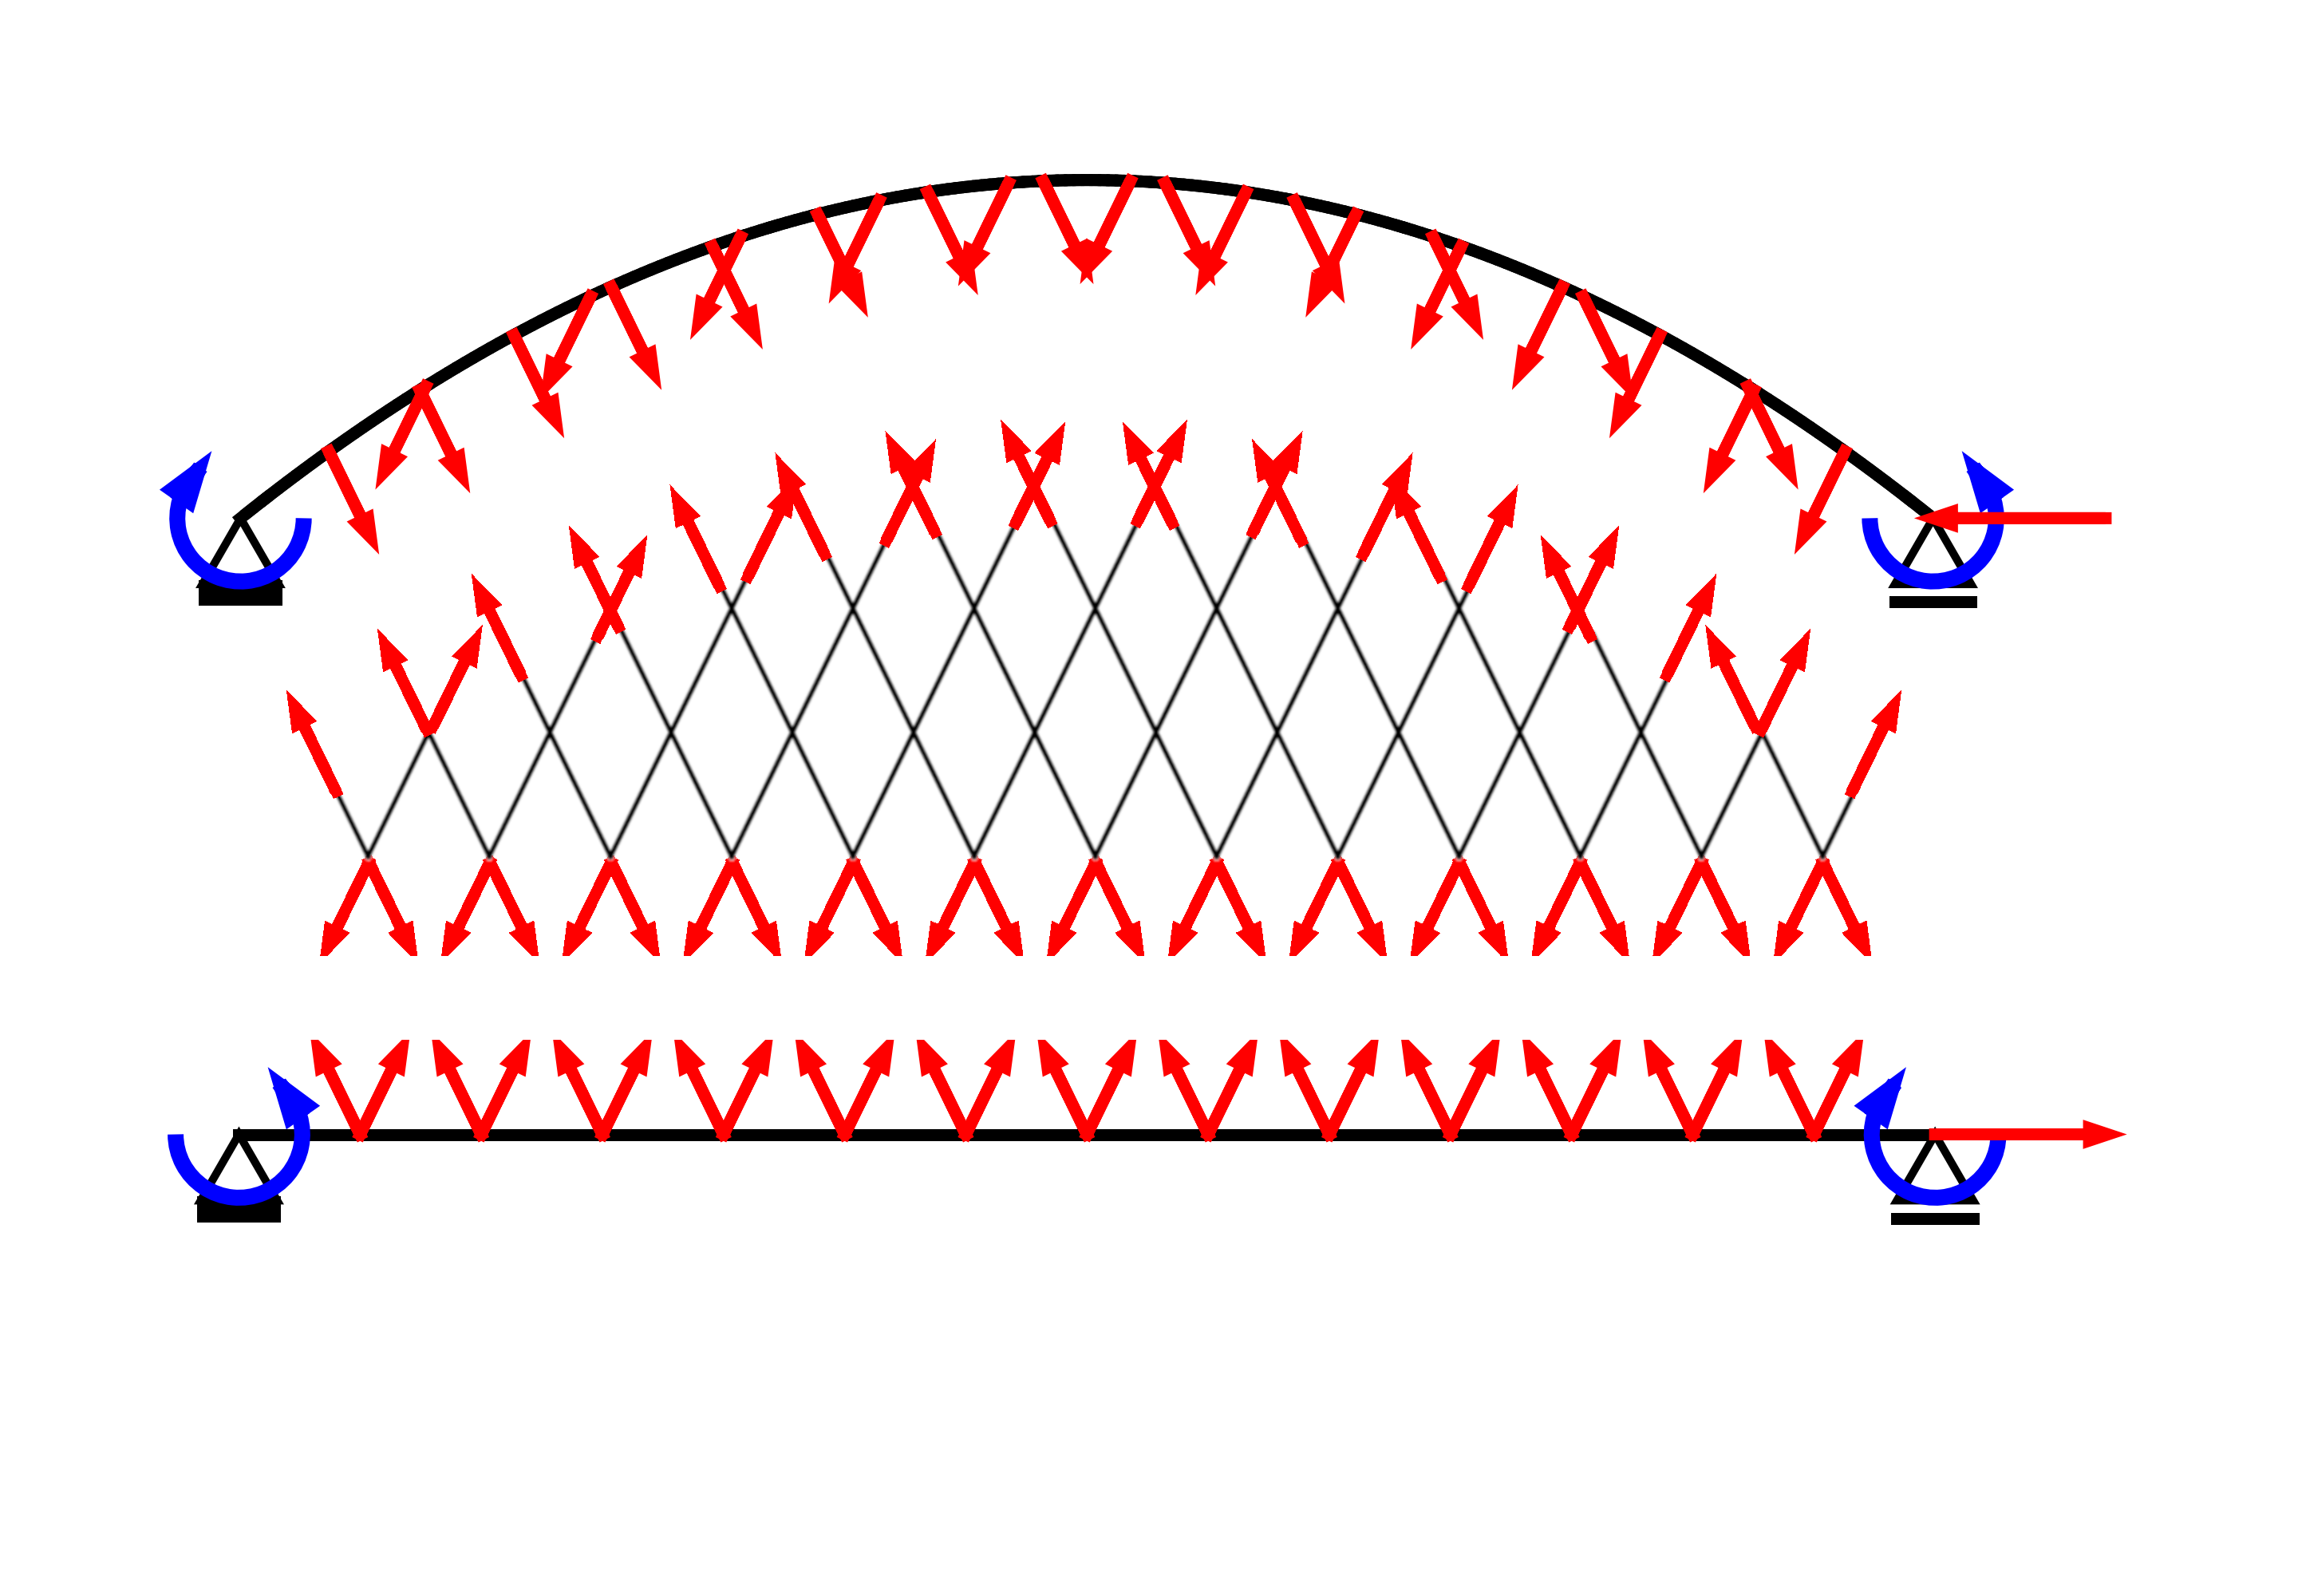
\includegraphics[trim={1cm 16cm 4cm 6.5cm},clip, width=0.65\textwidth]{overleaf/Pictures/Supernumerary forces.png}
    \caption{Set of supernumerary forces in the structural model}
    \label{fig:super_forces}
\end{figure}

For the Blennerhassett Island Bridge, 29 independent self-equilibrium stress states are present, one for each hanger and three for the arch and the tie. Under consideration of symmetry, 15 independent states remain. Instead of the hypothetical residual stress state under no loads, the state under permanent loads is investigated in this Thesis. Thereby, the residual stresses are defined indirectly. 
For the investigation of the stress state under permanent loads, the structural model of the network arch bridge can be split into the tie and the arch. If the forces at the knuckle and in the hangers are consistent, they can ultimately be recombined to form the permanent state of the network arch.
For general circumstances, including unsuitable arch shapes and hanger arrangements, it is a challenging task to find appropriate permanent hanger forces. This task is usually tackled by the engineer through trial and error, as it was the case for the design of the Blennerhassett Island Bridge. The respective result is neither reproducible nor can it claim optimality. In this Section, a few methods with a variety of applications are presented. 


\subsection{Zero-displacement method}
The zero-displacement method gives a first estimation of the hanger forces and is often used for the more popular cable-stayed bridge type. The permanent hanger forces are determined from a structural analysis of the tie girder where at every hanger connection a vertical support is introduced. In this way, the moment distribution in the tie is adequately balanced and creeping effects do not change the moment distribution. For a network tied-arch bridge, additionally to the supports at the connection nodes, a fully fixed support can be introduced at the knuckle. It represents the connection of the tie girder to the arch rib and gives the permanent moment between the two, which has also been considered part of the supernumerary set. The model of the tie resembles a multi span beam, as shown in Figure \ref{fig:zero_disp}. For the case of a network tied-arch bridge, multiple hangers can connect to the tie at a particular node and the vertical forces have to be distributed between the respective hangers. One option is to assign forces of equal magnitude to each of the hangers resulting in the intended vertical force. 

\begin{figure}[H]
    \centering
    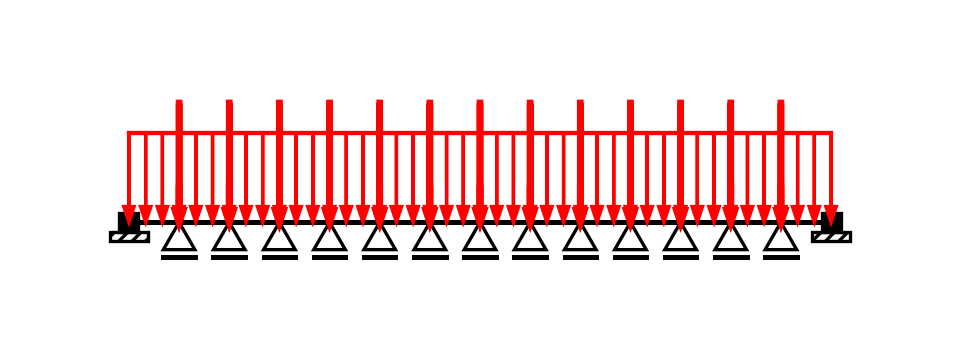
\includegraphics[trim={0 1cm 0 1cm},clip,width=0.6\textwidth]{illustrations/optimisation methods/zero-displacement.png}
    \caption{Zero-displacement method on the tie girder}
    \label{fig:zero_disp}
\end{figure}

In a second step, the hanger forces and the constraint moment at the knuckle are applied to the arch to determine its permanent state. Thereby the arch is affected by a significant moment distribution with the peak at the crown of $M_{p,crown}$. Additionally, the permanent tie tension force, which has a decisive influence on the arch, can be chosen freely at this point as it was neglected in the investigation of the tie girder. As a simplistic approach, the permanent tie tension force $N_{p,Tie}$ can be calculated to cause a disappearing moment at the crown of the arch according to Equation \ref{eq:M_0}. Otherwise, the more elaborate methods in the followings Sections can be used to determine this last supernumerary force.

\begin{equation}
    N_{p,Tie} = \frac{M_{p,crown}}{r}
    \label{eq:M_0}
\end{equation}

This approach is fast and simple to calculate. For a standard hanger arrangement and an adapted arch shape, these simple approaches yield adequate permanent moment distributions. However, for a radial hanger arrangement, in which the hanger connections do not coincide with the floor beams, or for a specific arch shape that does not resemble the respective thrust line, the zero-displacement method does not yield a useful self-equilibrium stress state.

\subsection{Moment minimisation}
It is the goal of an efficient initial configuration to simplify the design verifications by counteracting the effects expected in the various load cases. For the moment minimisation method, this is achieved by minimising the permanent moment distribution in the tie and potentially the arch as well. The permanent moment distribution at m points along the considered component $M \in \mathbb{R}^m$ can be described by Equation \eqref{eq:perm_mom}. 
\begin{equation}
    {\bf M} = {\bf M_0} + \sum_{i=1}^{n} {\bf M_i} \cdot X_i = {\bf M_0} + {\bf M_{sn}} \cdot {\bf X}
    \label{eq:perm_mom}
\end{equation}
where ${\bf M_0} \in \mathbb{R}^m$ is the moment distribution of the permanent loads on the basic system, ${\bf M_i} \in \mathbb{R}^m$ is the moment distribution of the i-th supernumerary unit force, ${X_i} \in \mathbb{R}$ is the i-th supernumerary force. The latter two can be combined into the matrix of supernumerary moment distributions ${\bf M_{sn}} \in  \mathbb{R}^{m\times n}$ and the vector of supernumerary forces or moments ${\bf X} \in \mathbb{R}^n$. An example of a supernumerary hanger force and its moment distribution is shown in Figure \ref{fig:Minimisation}.

\begin{figure}[H]
\centering
\begin{subfigure}{0.5\textwidth}
    \centering
    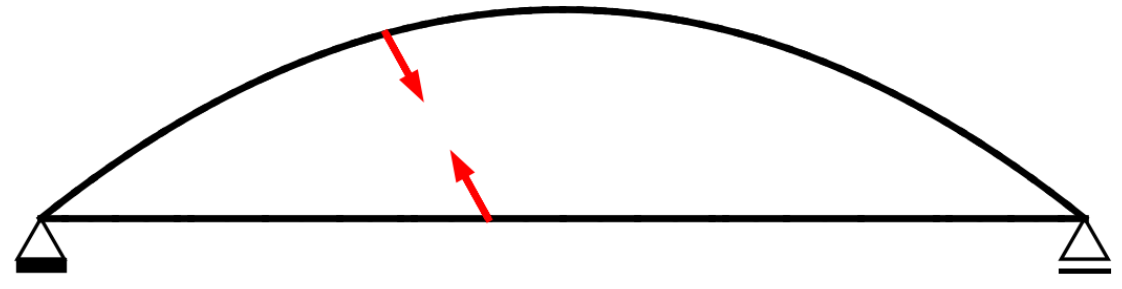
\includegraphics[trim={0 0cm 0 0},clip, width=0.9\textwidth]{overleaf/Appendix/Pictures/min_1.PNG}
    \caption{Basic system and supernumerary force}
    \label{fig:Minimisation_1}
\end{subfigure}%
\begin{subfigure}{.5\textwidth}
    \centering
    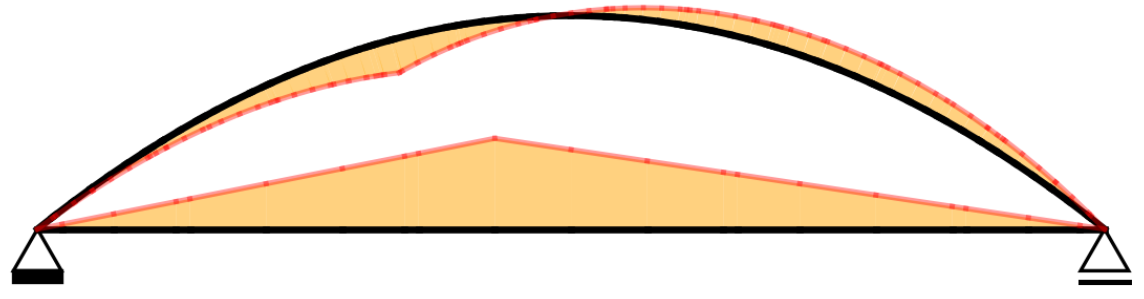
\includegraphics[trim={0 0cm 0 0},clip, width=0.9\textwidth]{overleaf/Appendix/Pictures/min_2.PNG}
    \caption{Moments under supernumerary force}
    \label{fig:Minimisation_2}
\end{subfigure}
\caption{Moment distribution of supernumerary force}
\label{fig:Minimisation}
\end{figure}

\newpage
The problem of minimising the absolute maximum moments can be formulated according to Equation \eqref{eq:minimisation}, where the absolute maximum moment is expressed also as the infinity norm.
\begin{align}
    \underset{{\bf X}}{\text{Minimize}} \quad & f({\bf X}) = \max({\bf M}, -{\bf M}) = \|{\bf M_0} + {\bf M_{sn}} \cdot {\bf X}\|_{\infty} 
    \label{eq:minimisation}
\end{align}
With the helper variable $t$, the previously stated problem can be formulated as a linear programming problem, as shown in Equation \eqref{eq:minimisation_2}.
The variable $t$ describes the moment magnitude which is larger than the all absolute moments in ${\bf M}$ according to the inequality conditions.
\begin{align}
    \underset{t, {\bf X}}{\text{Minimize}} \quad & f(t) = t \label{eq:minimisation_2} \\
    \text{s.t.} \quad & {\bf M_0} + {\bf M_{sn}} \cdot {\bf X} - t {\bf 1} \leq  0 \nonumber \\
    \quad & {-\bf M_0} - {\bf M_{sn}} \cdot {\bf X} - t {\bf 1} \leq 0 \nonumber
\end{align}
Additionally, bounds for the permanent hanger forces can be specified as further inequality conditions. It should be noted that under the consideration of symmetry the amount of variables in the linear problem can be reduced. If only the moment distribution in the tie is optimised, it makes sense to only consider vertical forces at each hanger node to obtain an unambiguous problem. In a second step, the optimised vertical forces are assigned to the two hangers at the node. The obtained problem is efficiently and reliably solvable as it is formulated as a linear programming problem. It can even be solved by Microsoft Excel without the need of additional software.

\subsection{Least squares of moments}
As an alternative approach, the supernumerary forces can be determined using the method of least squares. The objective of this method is to find supernumerary forces which counteract a certain moment distribution, for example the moment distribution on the basic system. Using the variables which were introduced in the previous section, the objective is described by Equation \eqref{eq:lsq_1}.
\begin{equation}
    {\bf M_{sn}} \cdot {\bf X} = -{\bf M_0}
    \label{eq:lsq_1}
\end{equation}
As this yields an overdetermined system, the equations cannot be solved simultaneously. Using the method of least squares, the sum of the squared deviations can be minimised by solving the determined system in Equation \eqref{eq:lsq_2}.
\begin{equation}
    ({\bf M_{sn}}^T\,{\bf M_{sn}}) \cdot {\bf X} = -{\bf M_{sn}}^T\,{\bf M_0}
    \label{eq:lsq_2}
\end{equation}
The drawback of this method is that no bounds for the hanger forces can be specified. However, this method is particularly useful, if the hanger forces have been optimised by minimising the moments on the tie girder. At this point, the permanent tension force in the tie girder is still undefined, as it does not affect the moment distribution. It can then be calculated by considering the moment distribution in the arch rib, minimising the squares of its moment distribution. In this case, the approach is fast and can even be solved without using linear algebra as there is only one variable.


\newpage
\section{Arch shape} \label{sec:met_arch}
The optimisation methods which were introduced in the previous chapter allow finding an efficient self-equilibrium stress state for a given arch shape. This corresponds to finding hanger forces with a resulting thrust line close to the predefined arch shape. However, a more elegant solution would be an adaptation of the arch shape to the thrust line under permanent loads. There are two thrust line derivations relevant for this Thesis. In Section \ref{app:continuous}, the thrust line is derived for the hypothetical case of an infinitely dense hanger arrangement. For a discrete hanger arrangement the thrust line can be derived according to the method described in Section \ref{app:discrete}. Both methods take the weight of the arch into account.

\subsection{Thrust line of continuous hanger arrangement}\label{app:continuous}
In a first step, the hanger force densities of each hanger set are determined without the consideration of the arch. There are multiple possibilities to do so. For example, they could be calculated to be in equilibrium with the permanent vertical force $q$, depending on their angles of inclination $\alpha$ and $\beta$. However, horizontal equilibrium is an unnecessary condition, as the tie is affected by significant tension forces anyway. Therefore, it is proposed to assign force densities of identical magnitude to hangers on each infinitesimal element, as illustrated in Fig. \ref{fig:continuous_1}. Also the resultant forces $F_L$ and $F_R$ are shown.
\begin{figure}[H]
    \centering
    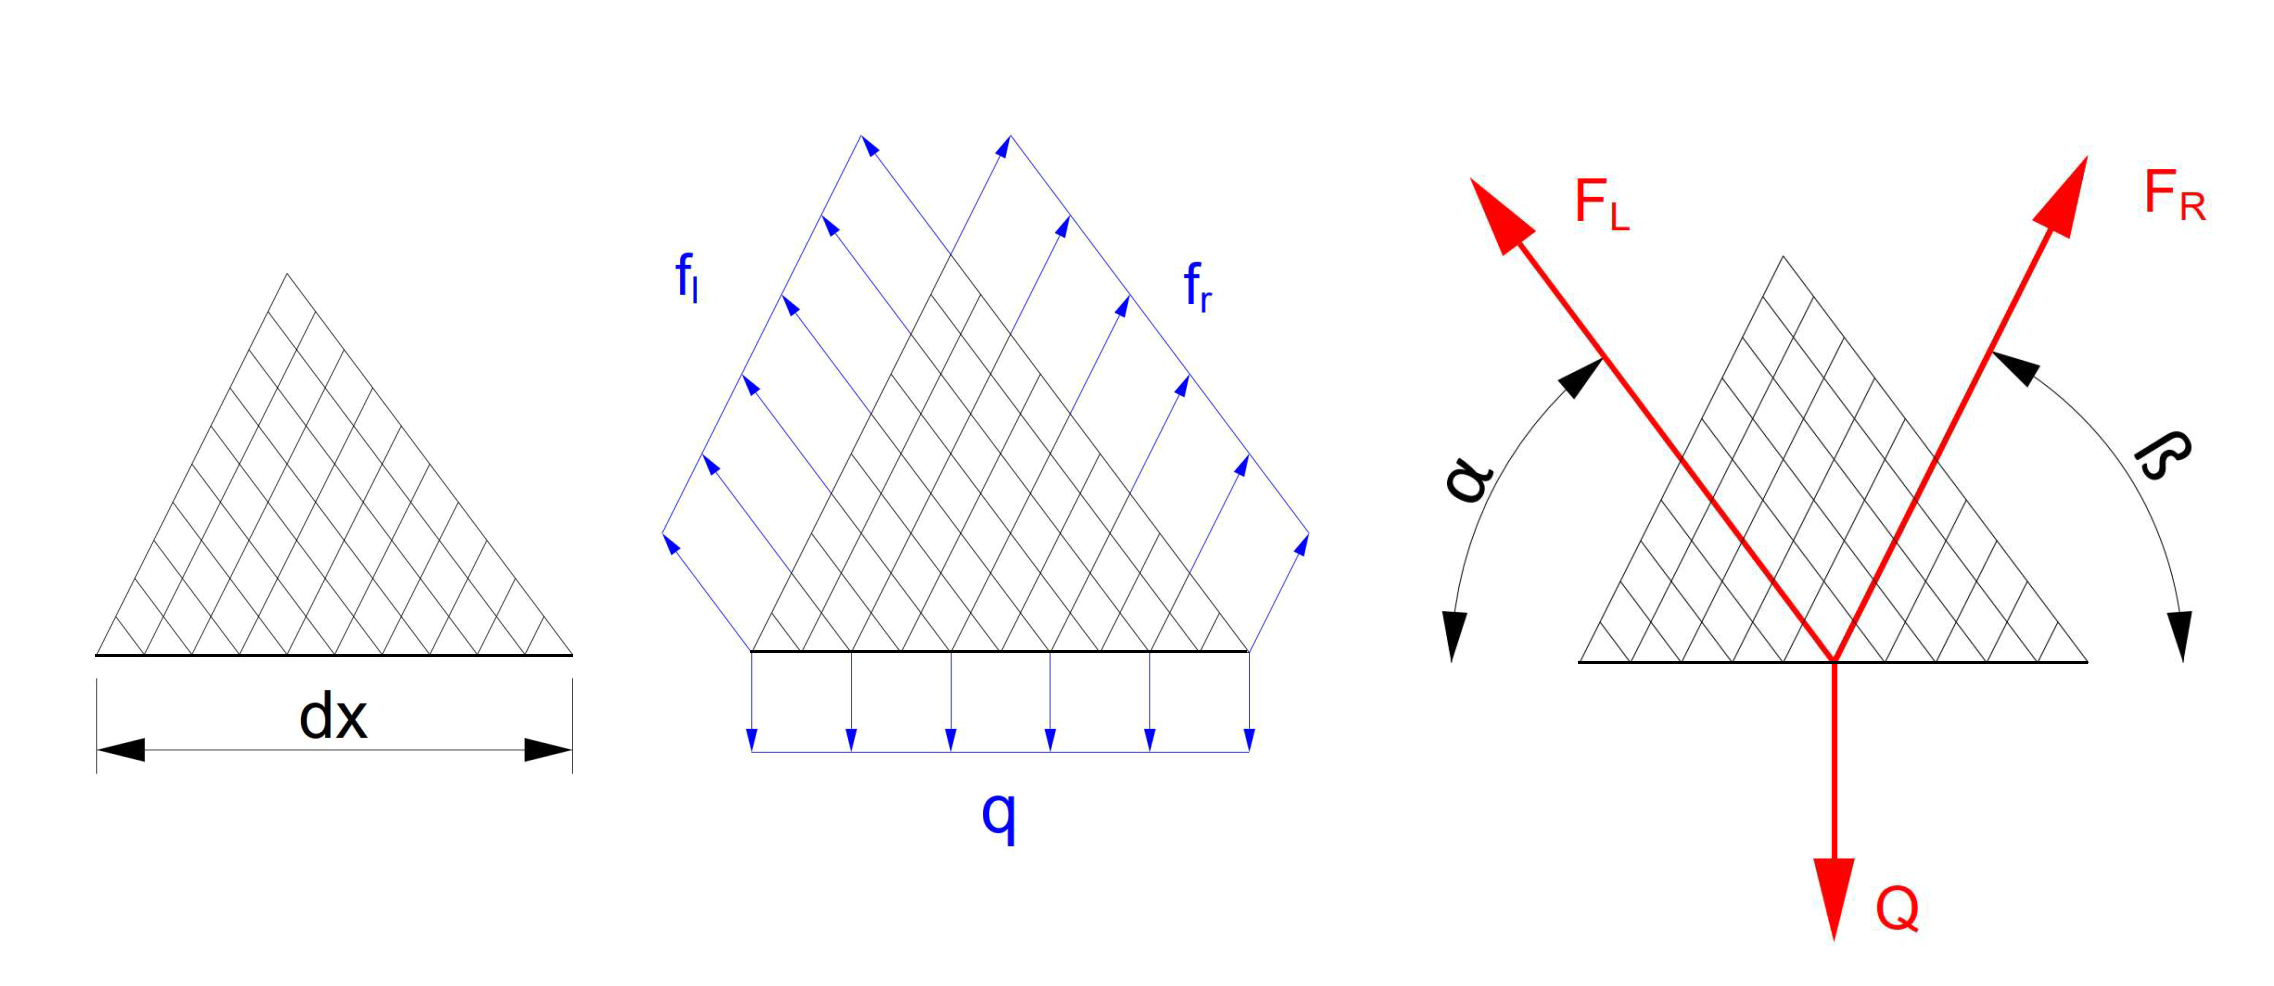
\includegraphics[width=0.8\textwidth]{overleaf/Appendix/Pictures/continuous_thrust_line_1.PNG}
    \caption{Hanger force densities on an infinitesimal element}
    \label{fig:continuous_1}
\end{figure}

The corresponding hanger force densities $f_l$ and $f_r$ can be calculated according to Eq. \eqref{eq:continuous_1}.
\begin{equation}
    f_l=f_r=\frac{q}{\sin{\alpha}+ \sin{\beta}}
    \label{eq:continuous_1}
\end{equation}

While the thrust line can be described analytically by a differential equation, it is impossible to get an analytical solution for general hanger arrangement patterns. Therefore, the thrust line of the infinitesimal hanger arrangement is calculated in fixed horizontal steps of $dx$ starting from the crown, where a normal force $N_{crown}$ is assumed. If the step $dx$ is small, it can be assumed, that the inclination of the thrust line undergoes small changes in every step. At the beginning of each step the normal force $N_1$ is known, which also corresponds to the inclination of the thrust line. In each step, the change of height of the thrust line $dy$ is determined iteratively. It underlies the condition that the new inclination coincides with the inclination of the new normal force, which can be described by Eq. \ref{eq:continuous_2}.
\begin{equation}
    dy = \frac{dx}{2} \cdot \left(\frac{N_{1,y}}{N_{1,x}} + \frac{N_{2,y}}{N_{2,x}} \right)
    \label{eq:continuous_2}
\end{equation}

The new normal force $N_2$ is determined from force equilibrium considering the hanger forces and the self weight, both of which depend on $dy$. The self weight is determined from the length of the segment multiplied by the weight per meter. For the hanger forces, the lengths of the two hanger sets on the tie $dl_1$ and $dl_2$ affecting the considered arch segment are determined over geometrical considerations. Using the previously determined hanger force densities the resulting hanger force is determined. The calculation of a single step is illustrated in Fig. \ref{fig:continuous_2}.
\begin{figure}[H]
    \centering
    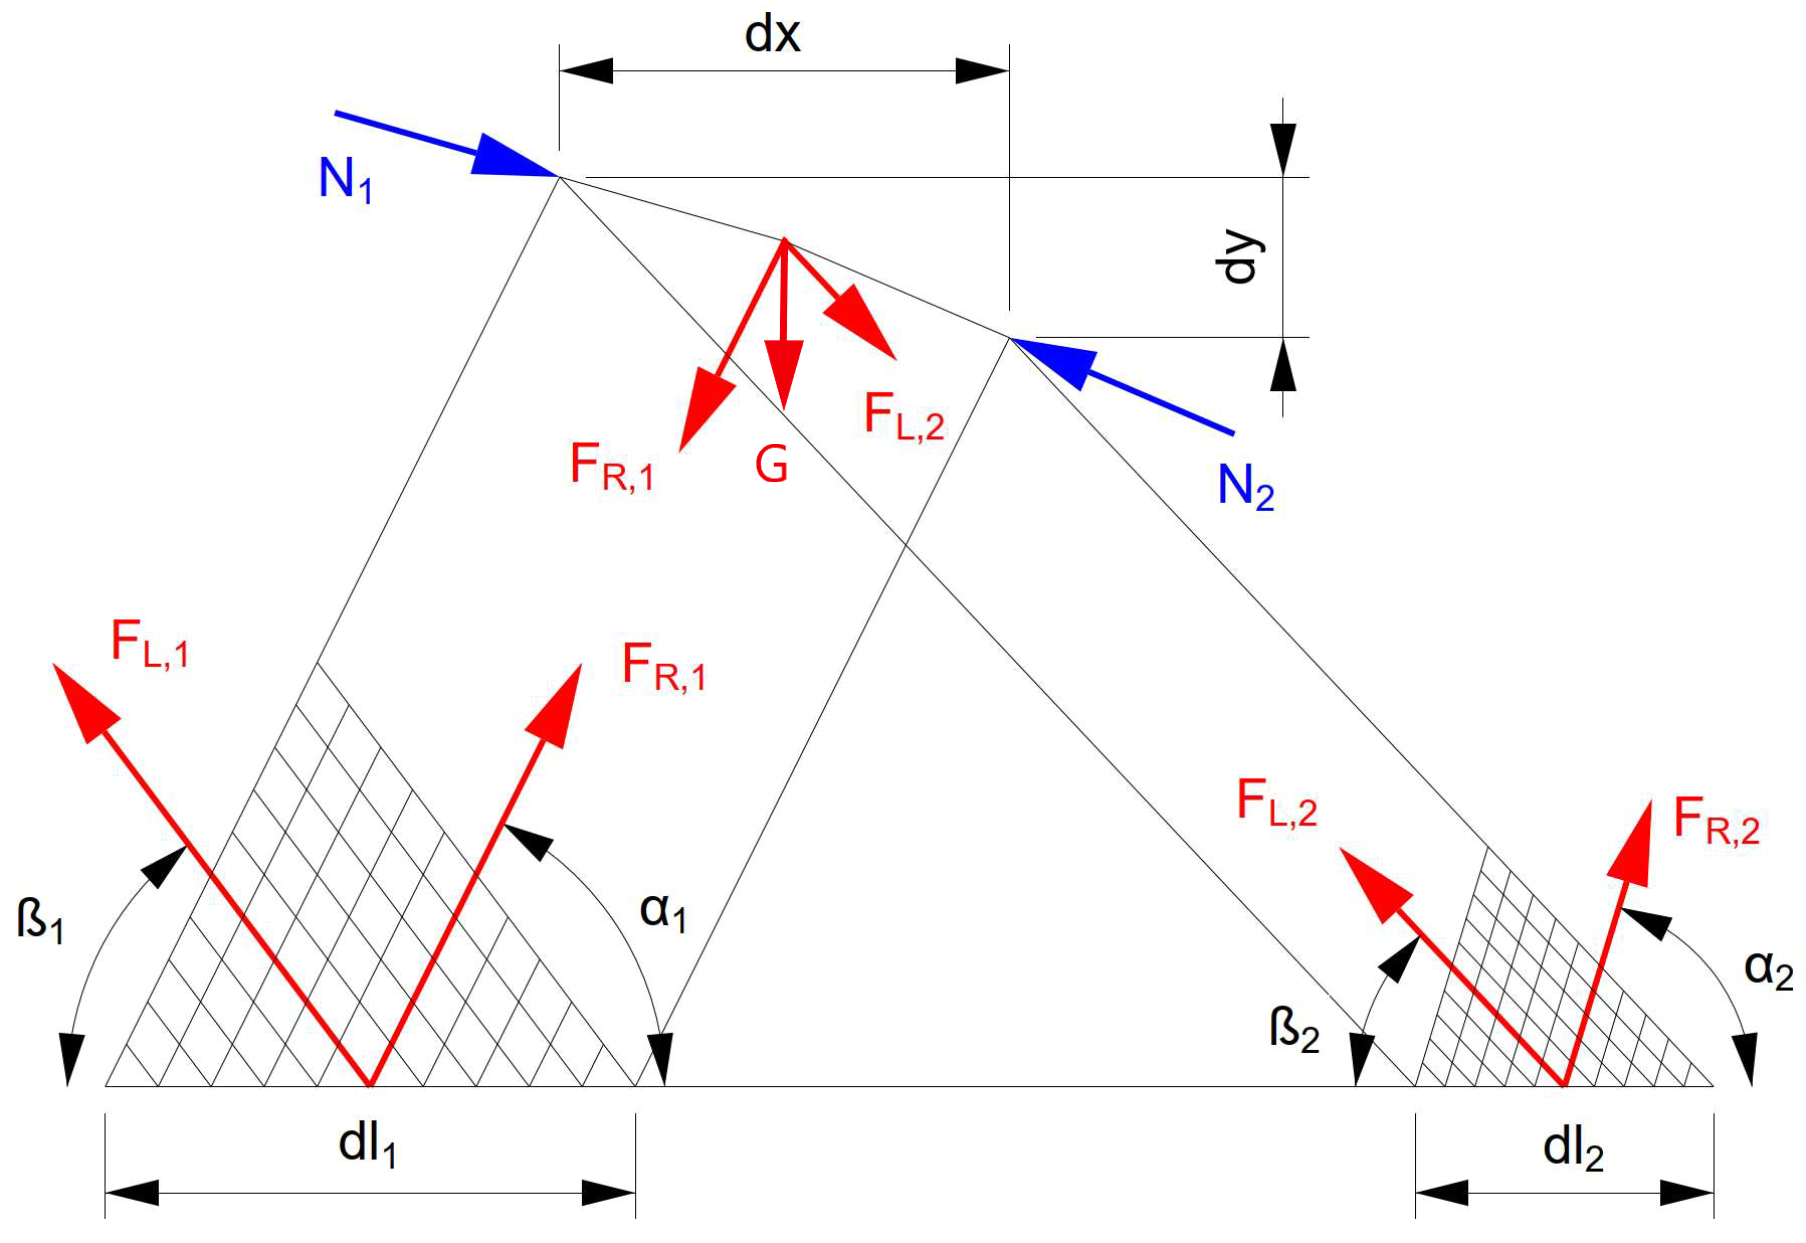
\includegraphics[width=0.6\textwidth]{overleaf/Appendix/Pictures/continuous_thrust_line.PNG}
    \caption{Derivation of the arch thrust line for a continuous hanger arrangement}
    \label{fig:continuous_2}
\end{figure}

Ultimately, the normal force in the crown $N_{crown}$ is determined iteratively for the thrust line to intersect the knuckle point. However, this normal force in the crown could also be determined from static considerations involving global longitudinal moment and the hanger force densities without the need of an iteration.


\subsection{Thrust line of discrete hanger arrangement}\label{app:discrete}

Calculating the thrust line of a discrete hanger arrangement is a particular challenge as it is not known in which order the hangers intersect the thrust line beforehand. Therefore it is also calculated in steps. Similar to the continuous calculation, it is started from the crown with an estimated normal force $N_{crown}$ and the inclination at the beginning of every step corresponds to the ratio of the normal force components. Further, the arch's weight per horizontal meter is estimated from Eq. \ref{eq:g_arch}.

\begin{equation}
    g_{arch,x} = g_{arch} \cdot \sqrt{1+y'^2} = g_{arch} \cdot \sqrt{1+\left( \frac{N_{y}}{N_{x}} \right)^2}
    \label{eq:g_arch}
\end{equation}

Using this weight per horizontal meter, the parabolic thrust line can be estimated according to Eq. \ref{eq:discrete}. The height at the beginning of the current step is given by $y_1$ The second term gives the inclination of the normal force, which would continue the thrust line under no additional loading. The weight of the arch causes a slight curvature according to the third quadratic term.

\begin{equation}
    y(x) = y_1 - \frac{N_y}{N_x} \cdot x - \frac{g_{arch,x}}{2\cdot N_x}\cdot x^2
    \label{eq:discrete}
\end{equation}

Unless a hanger intersects the thrust line within the current step, the thrust line is continued by the step length $dx$. An illustration is given in Fig. \ref{fig:discrete_1}.

\begin{figure}[H]
    \centering
    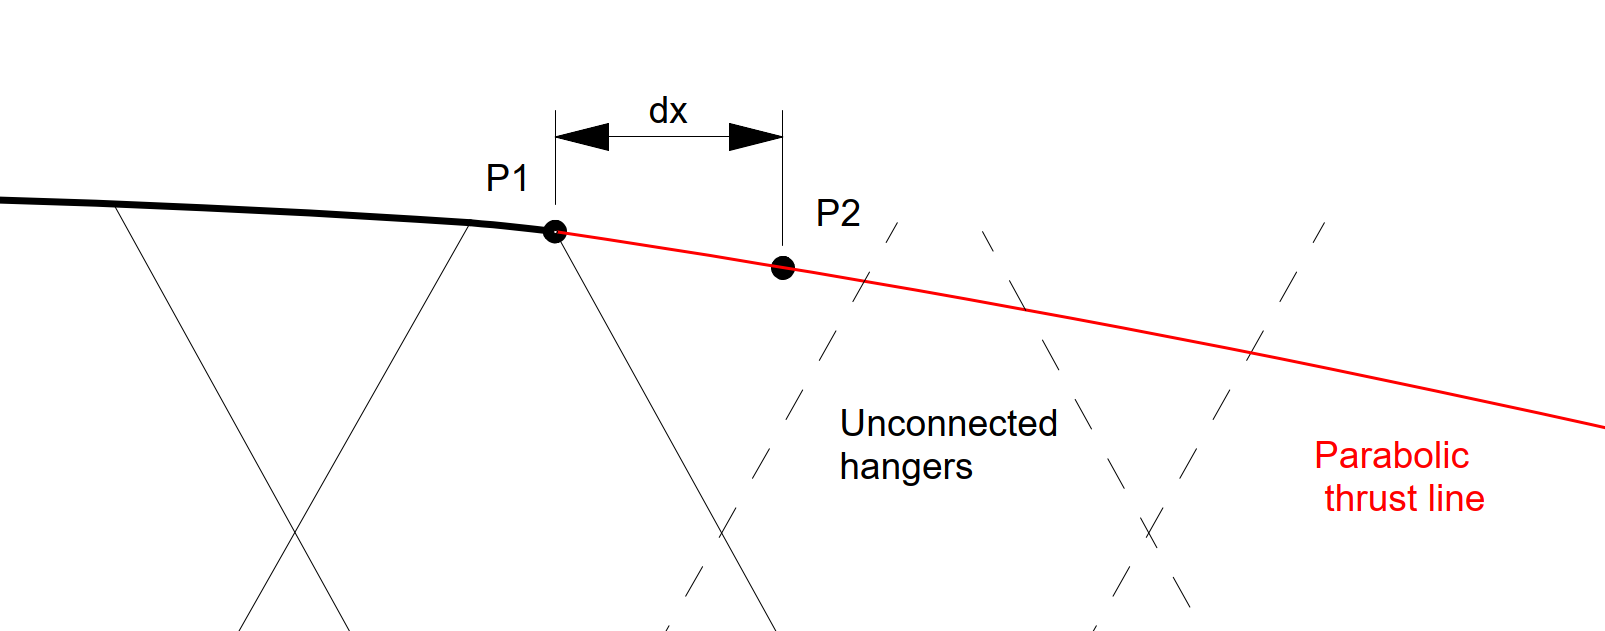
\includegraphics[width=0.7\textwidth]{overleaf/Appendix/Pictures/discrete_thrust_line_1.PNG}
    \caption{Thrust line derivation step without intersecting hangers}
    \label{fig:discrete_1}
\end{figure}

However, if a hanger intersects the thrust line within the current step, this intersection point is added to the thrust line and used as a starting point for the next step. This step is illustrated in Fig. \ref{fig:discrete_2}.

\begin{figure}[H]
    \centering
    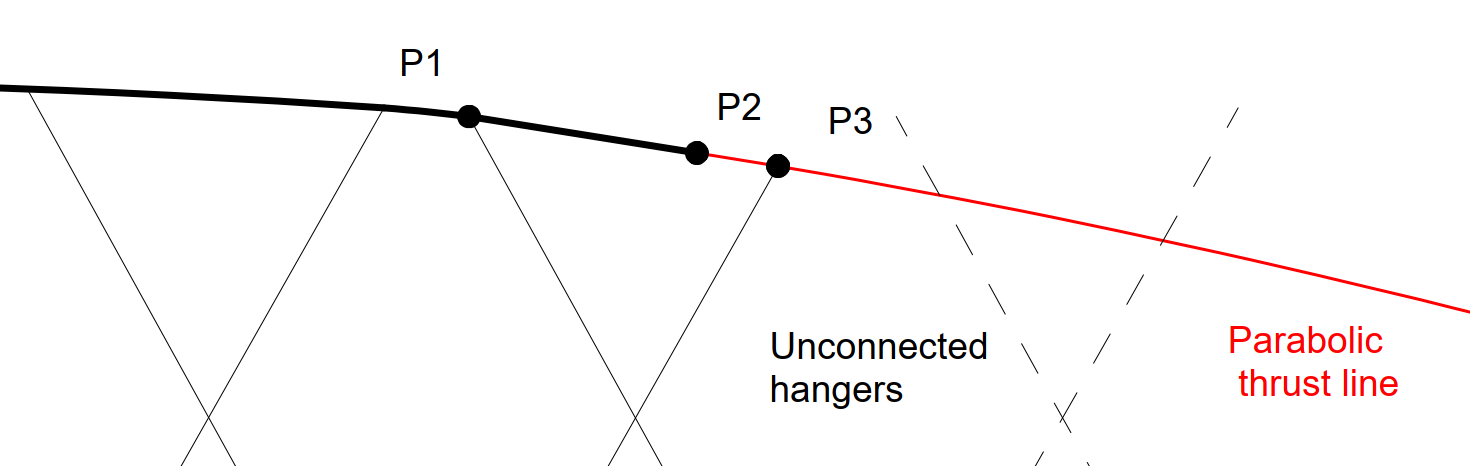
\includegraphics[width=0.7\textwidth]{overleaf/Appendix/Pictures/discrete_thrust_line_2.PNG}
    \caption{Thrust line derivation step connecting to the next hanger}
    \label{fig:discrete_2}
\end{figure}

Again, the normal force in the crown $N_{crown}$ is determined iteratively for the thrust line to intersect the knuckle point. Numerically, it would be much easier to calculate it from static considerations.

\subsection{Polynomial approximation}

\newpage
\section{Design verifications} \label{sec:met_ver}
To ensure a safe and reliable structure, the limit states for strength, extreme events and fatigue are considered \cite{AASHTO}.  The resulting demand over capacity ratios (D/C) will also be used in Section \ref{sec:met_cost} for an estimation of the cost function.

\subsection{Strength limit states}
The strength limit states are considered to ensure that the design of the structure guarantees enough strength and stability for the highest expected loads in its life cycle. The load combinations considered in this investigation are related to the main actions of vehicular use (Strength-I), wind exposure (Strength-III) and a load combination for heavy bridges (Strength-IV). The load factors used for each strength limit state are presented in Table \ref{tab:uls_combination}. For the permanent loads DC and DW, two factors are given out of which the one impeding to the verification is taken. For the locked-in erection stresses no variability is taken into account.

\begin{table}[H]
\caption{Load combinations for the ultimate limit state}
\centering
\begin{tabular}{lccccc}
\hline
Load         & EL  & DC         & DW         & LL   & WS  \\ \hline
Strength-I   & 1.0 & 0.9 / 1.25 & 0.65 / 1.5 & 1.75 & -   \\
Strength-III & 1.0 & 0.9 / 1.25 & 0.65 / 1.5 & -    & 1.4 \\ 
Strength-IV  & 1.0 & 0.65 / 1.5 & 0.65 / 1.5 & -    & - \\ \hline
\end{tabular}
\end{table}

The arch and the tie are verified according to Equation \eqref{eq:design_verification}, neglecting the secondary force effects. For the hangers, enough resistance is proved if the highest stresses are below 65\% of the nominal capacity. 

\begin{equation}
    \frac{N_{Ed}}{N_{Rd}} + \frac{8.0}{9.0}\, \left(\frac{M_{y,Ed}}{M_{y,Rd}}+\frac{M_{z,Ed}}{M_{z,Rd}} \right) \leq 1.0
    \label{eq:design_verification}
\end{equation}

For simplicity, the value given by the left side of this condition is also referred to as the demand over capacity ratio for the arch and the tie.
%For the Blennerhassett Island Bridge, the DOC is evaluated according to this simplified verification. The obtained values are presented in Table [], along with the ratios taken from the design drawings in parenthesis. 

\subsection{Extreme event limit states}
Extreme events are unique circumstances whose return periods can be significantly greater than the life expectancy of the structure. In these events, the requirement for the bridge is its structural survival. In this investigation the extreme events of cable loss, cable replacement and tie fracture are examined. The load factors for each event is taken from the design drawings and presented in Table \ref{tab:extreme_combination}. For the events of cable loss and cable replacement, specific live loading arrangements (LL*) apply.

\begin{table}[H]
\caption{Load combinations for the extreme event limit states}
\label{tab:extreme_combination}
\centering
\begin{tabular}{lccccc}
\hline
Event         & EL  & DC         & DW         & LL*   & DAF  \\ \hline
Cable loss   & 1.0 & 1.2 & 1.4 & 0.75 & 1.75   \\
Cable replacement & 1.0 & 1.2 & 1.4 & 1.5 & 1.0 \\ 
Tie fracture  & 1.0 & 1.25 & 1.5 & 1.3 & - \\ \hline
\end{tabular}
\end{table}

For both hanger-related extreme events, each hanger is investigated individually according to the PTI (static) approach [cite PTI]. In a first step, the longitudinal live load arrangement, which maximises the respective hanger force, is determined. Therefor, The concentrated live load is always applied at the cross-girder closest to the considered hanger. The forces from the distributed live load are also arranged on a certain amount of neighbouring cross-girders, as illustrated in Figure \ref{fig:Cable_Loss_1}. The assumed hanger force before its replacement or loss is thereby determined. In a second step, the structural system is modified by removing the considered hanger. The hanger force is applied in opposite direction on the modified system, as shown in Figure \ref{fig:Cable_Loss_2}. The resulting effects are multiplied by a dynamic amplification factor (DAF) and superimposed on the effects from the state of maximised hanger force. The DAF for the event of cable loss is assumed to be 1.75.

\begin{figure}[H]
\centering
\begin{subfigure}{0.5\textwidth}
    \centering
    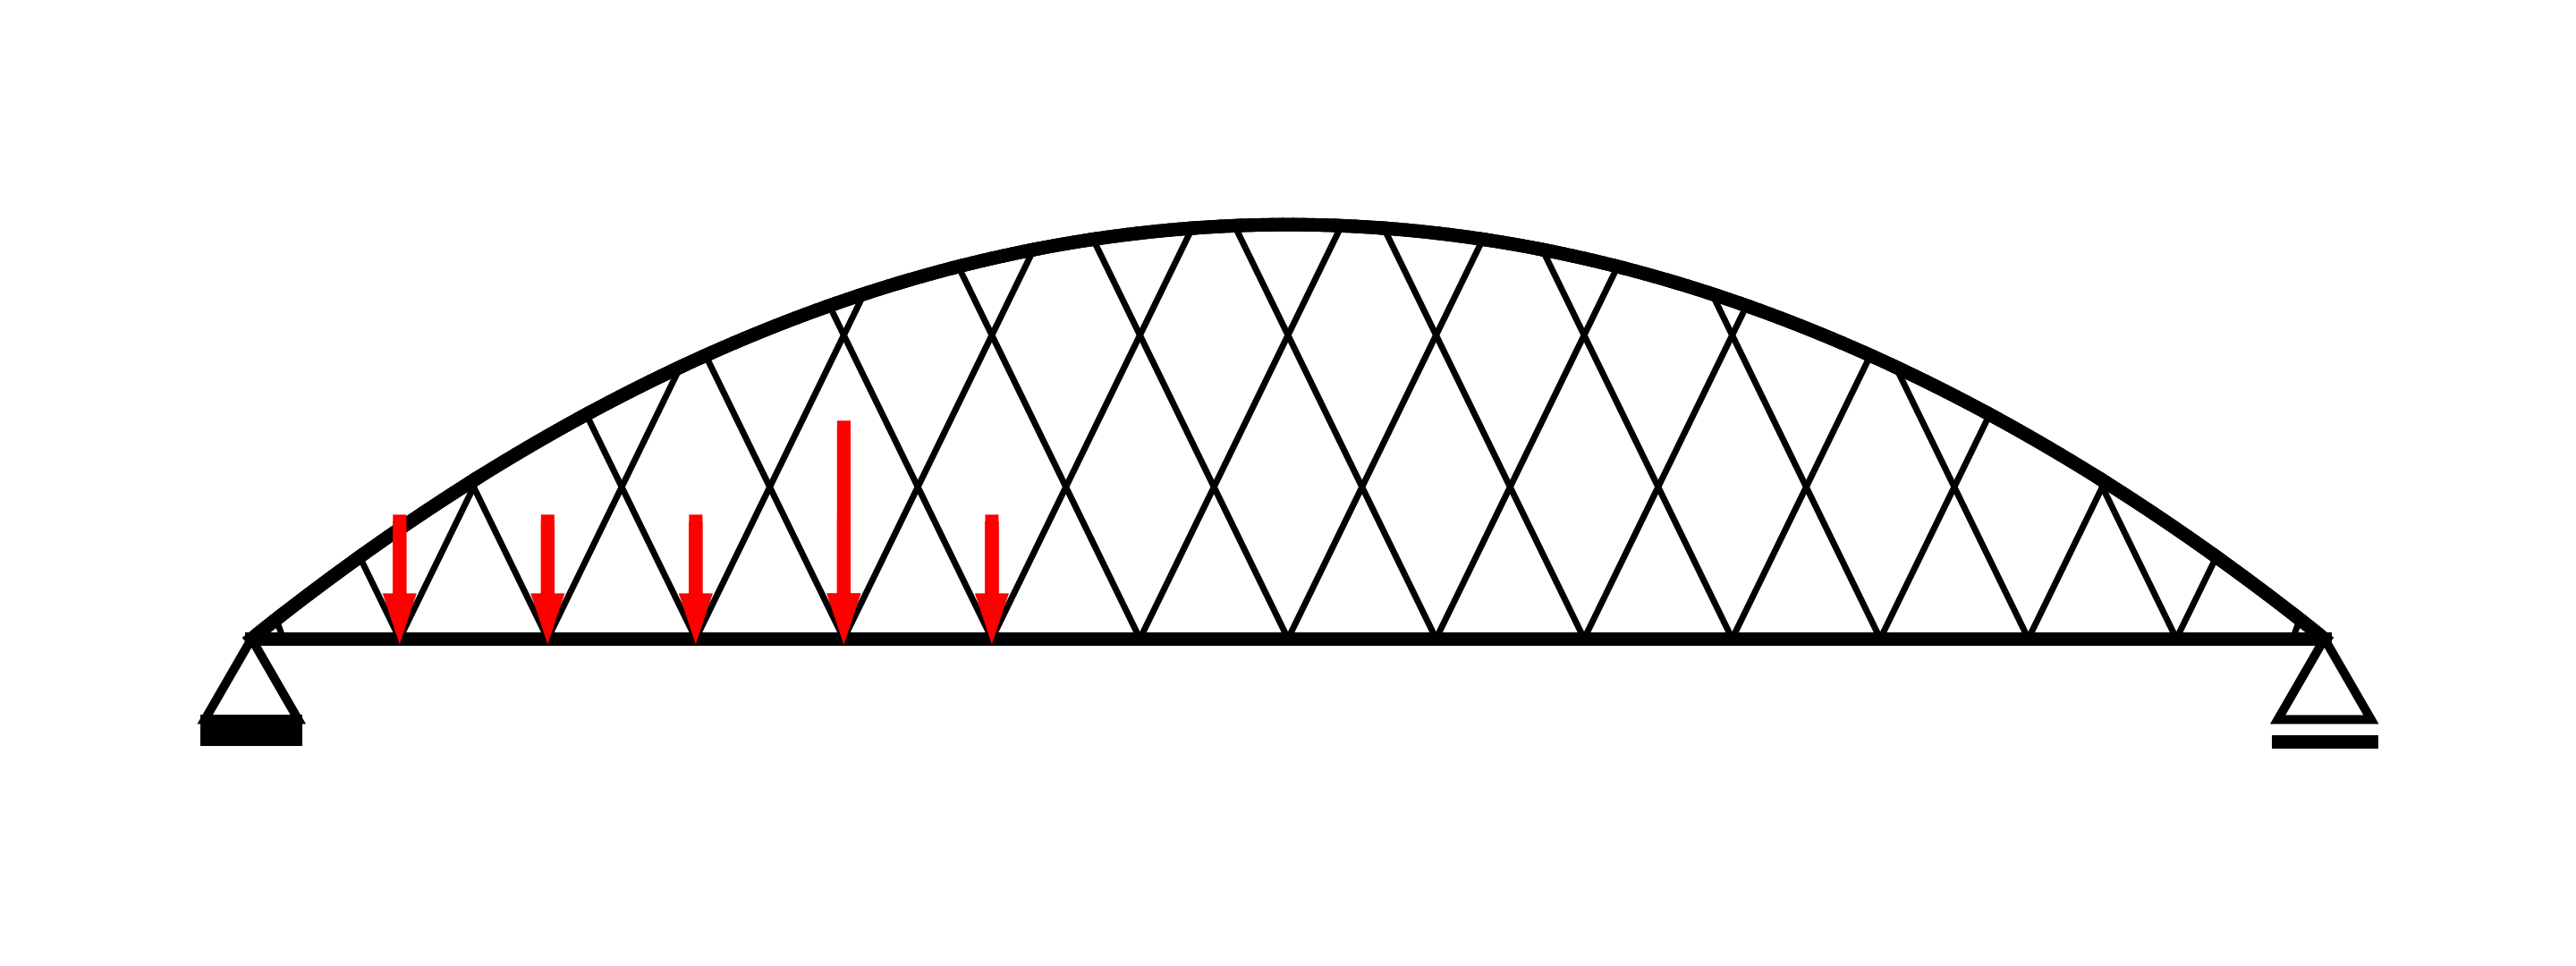
\includegraphics[trim={0 0.8cm 0 0.8cm},clip, width=0.9\textwidth]{illustrations/figures/cable loss - load arrangement.png}
    \caption{Live load arrangement to maximise hanger force}
    \label{fig:Cable_Loss_1}
\end{subfigure}%
\begin{subfigure}{.5\textwidth}
    \centering
    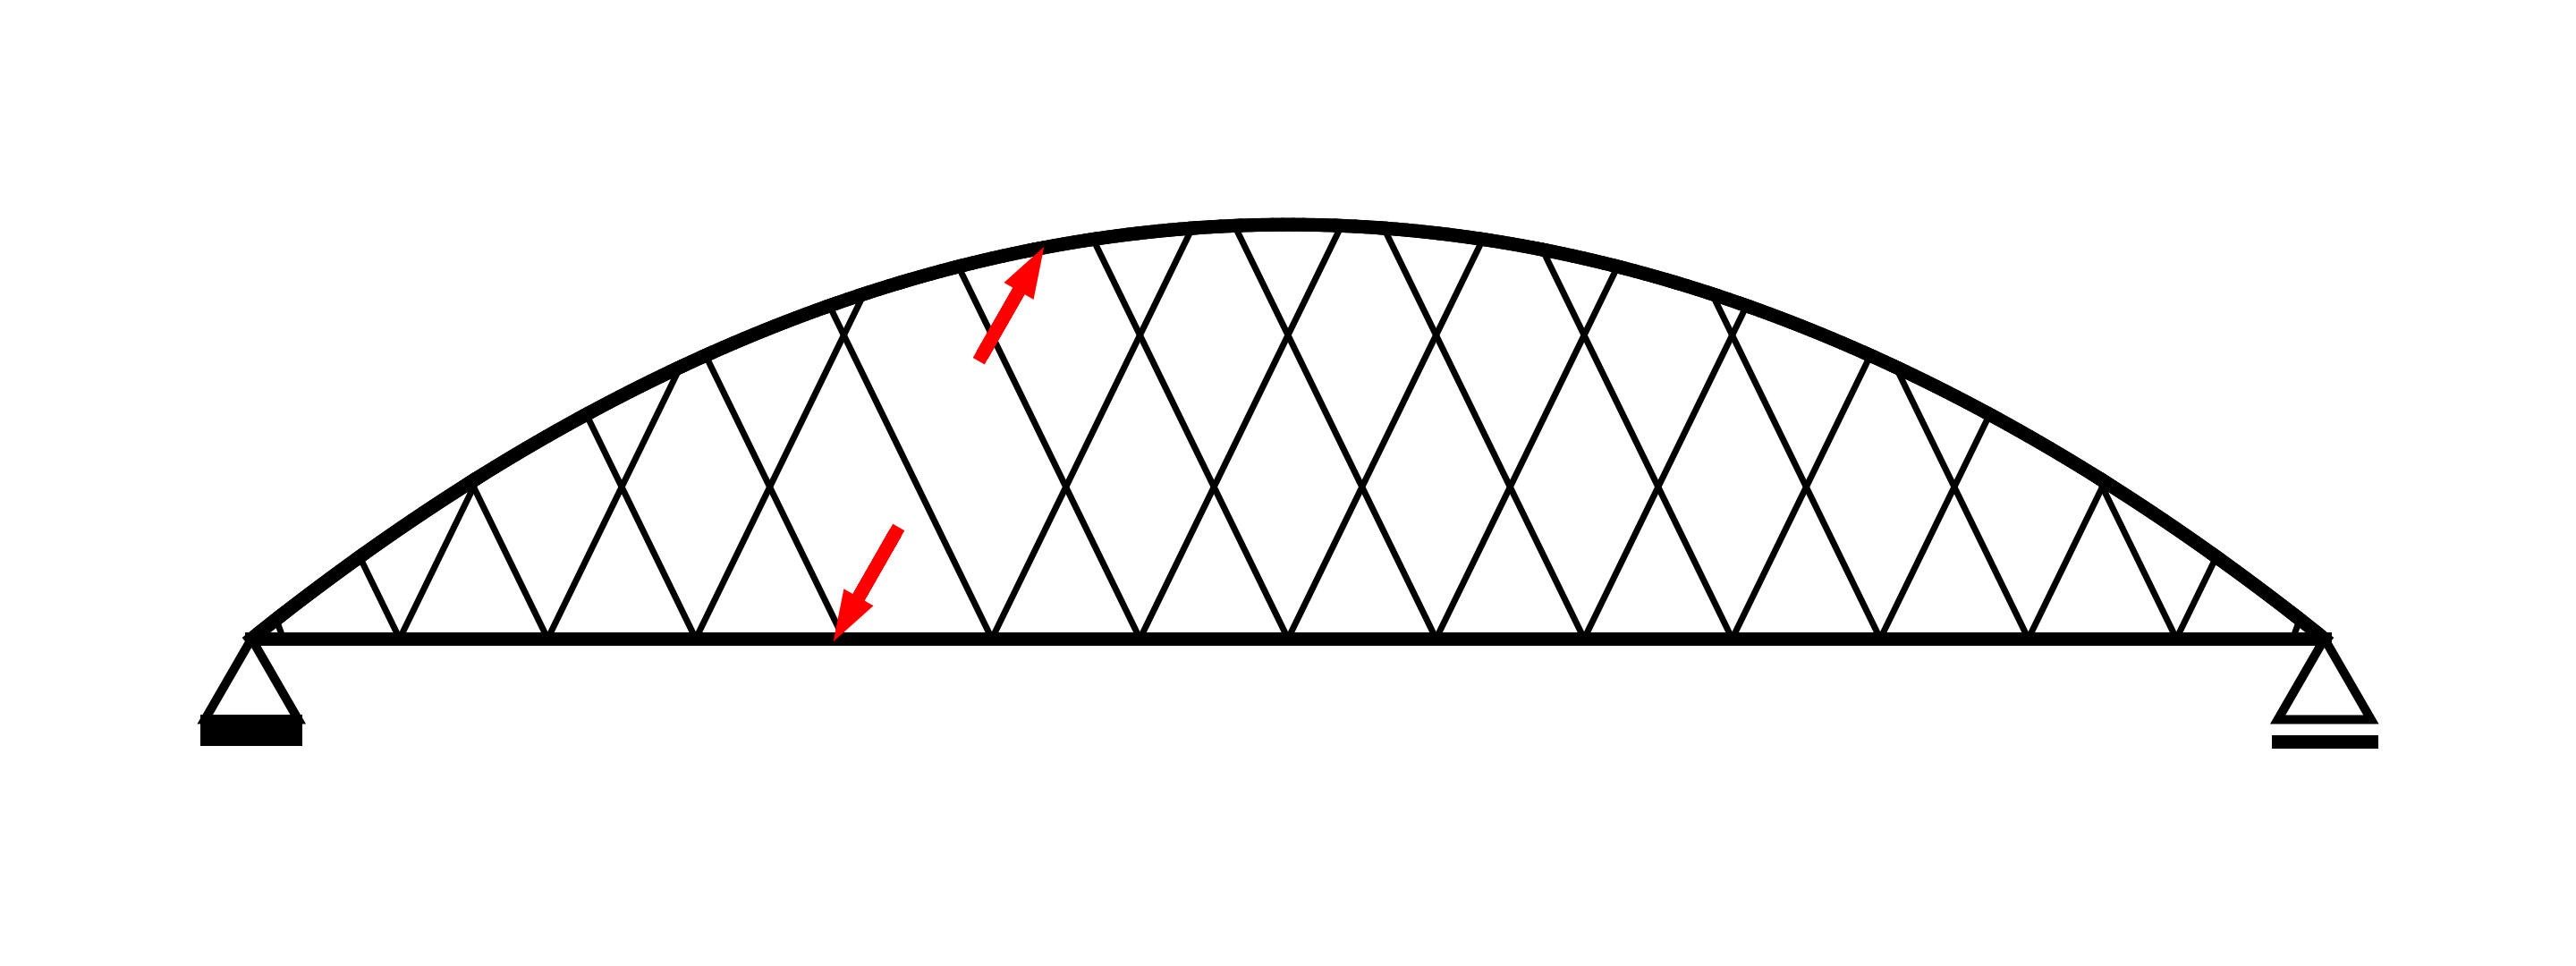
\includegraphics[trim={0 0.8cm 0 0.8cm},clip, width=0.9\textwidth]{illustrations/figures/cable loss.png}
    \caption{Structural model with opposite force}
    \label{fig:Cable_Loss_2}
\end{subfigure}
\caption{Calculation steps for loss of the fourth hanger}
\label{fig:Cable_Loss}
\end{figure}

[Tie fracture]

\subsection{Fatigue limit state}

\begin{table}[H] 
\caption{Cross-sectional resistances}
\centering
\begin{tabular}{lccc}
\hline
Segment & Normal force & Moment-y & Moment-z \\
 & [MN]   & [MNm] & [MNm] \\ \hline
Arch 1 & \SI{130.0}{} & \SI{78.7}{} & \SI{79.1}{}\\
Arch 2 & \SI{108.8}{} & \SI{71.5}{} & \SI{63.4}{}\\
Arch 3-4 & \SI{82.3}{} & \SI{50.0}{} & \SI{42.7}{}\\
Tie 1 & \SI{153.2}{} & \SI{100.8}{} & \SI{76.2}{}\\
Tie 2 & \SI{117.1}{} & \SI{82.8}{} & \SI{56.6}{}\\
Tie 3-4 & \SI{100.6}{} & \SI{76.2}{} & \SI{45.8}{}\\
Hangers & 4.19 & - & - \\\hline
\end{tabular}
\end{table}

\section{Estimation of cost function} \label{sec:met_cost}

\cleardoublepage

\chapter{Results}\label{sec:results}

\section{Base case}
As a reference for all following calculations, a model representing the Blennerhassett Island Bridge's final design is investigated. The results obtained by the analysis are then compared to the ones in the design drawings for plausibility. A particular challenge is the determination of the self-equilibrium stress state. As the arch was defined as an unsuitable parabola, appropriate hanger forces were determined by trial and error in the design. These permanent hanger forces of the final design are available in the drawings. However, they are inadequate for calculating the base case, as the load distribution in the model is simplified. Instead of another trial and error procedure for the base case, the hanger forces are obtained as the result of a simultaneous arch and tie moment optimisation. Thereby, the arch's moment is weighed by a factor of 1.5 to achieve an optimal similarity. Further, the hanger forces are bounded between 25\% and 45\% of their nominal strength. The base case's internal force distributions for the permanent state are shown in Fig. \ref{fig:base_case_permanent}. Instead of the normal force in the hangers, the demand over capacity ratio is shown directly. Only the hangers of one set are shown, namely the ones inclined to the right side, and the dots are connected for readability. As a comparison, the extreme values of each component, which are found in the design verifications in Appendix \ref{app:design_verifications}, are also shown.

\begin{figure}[H]
    \centering
    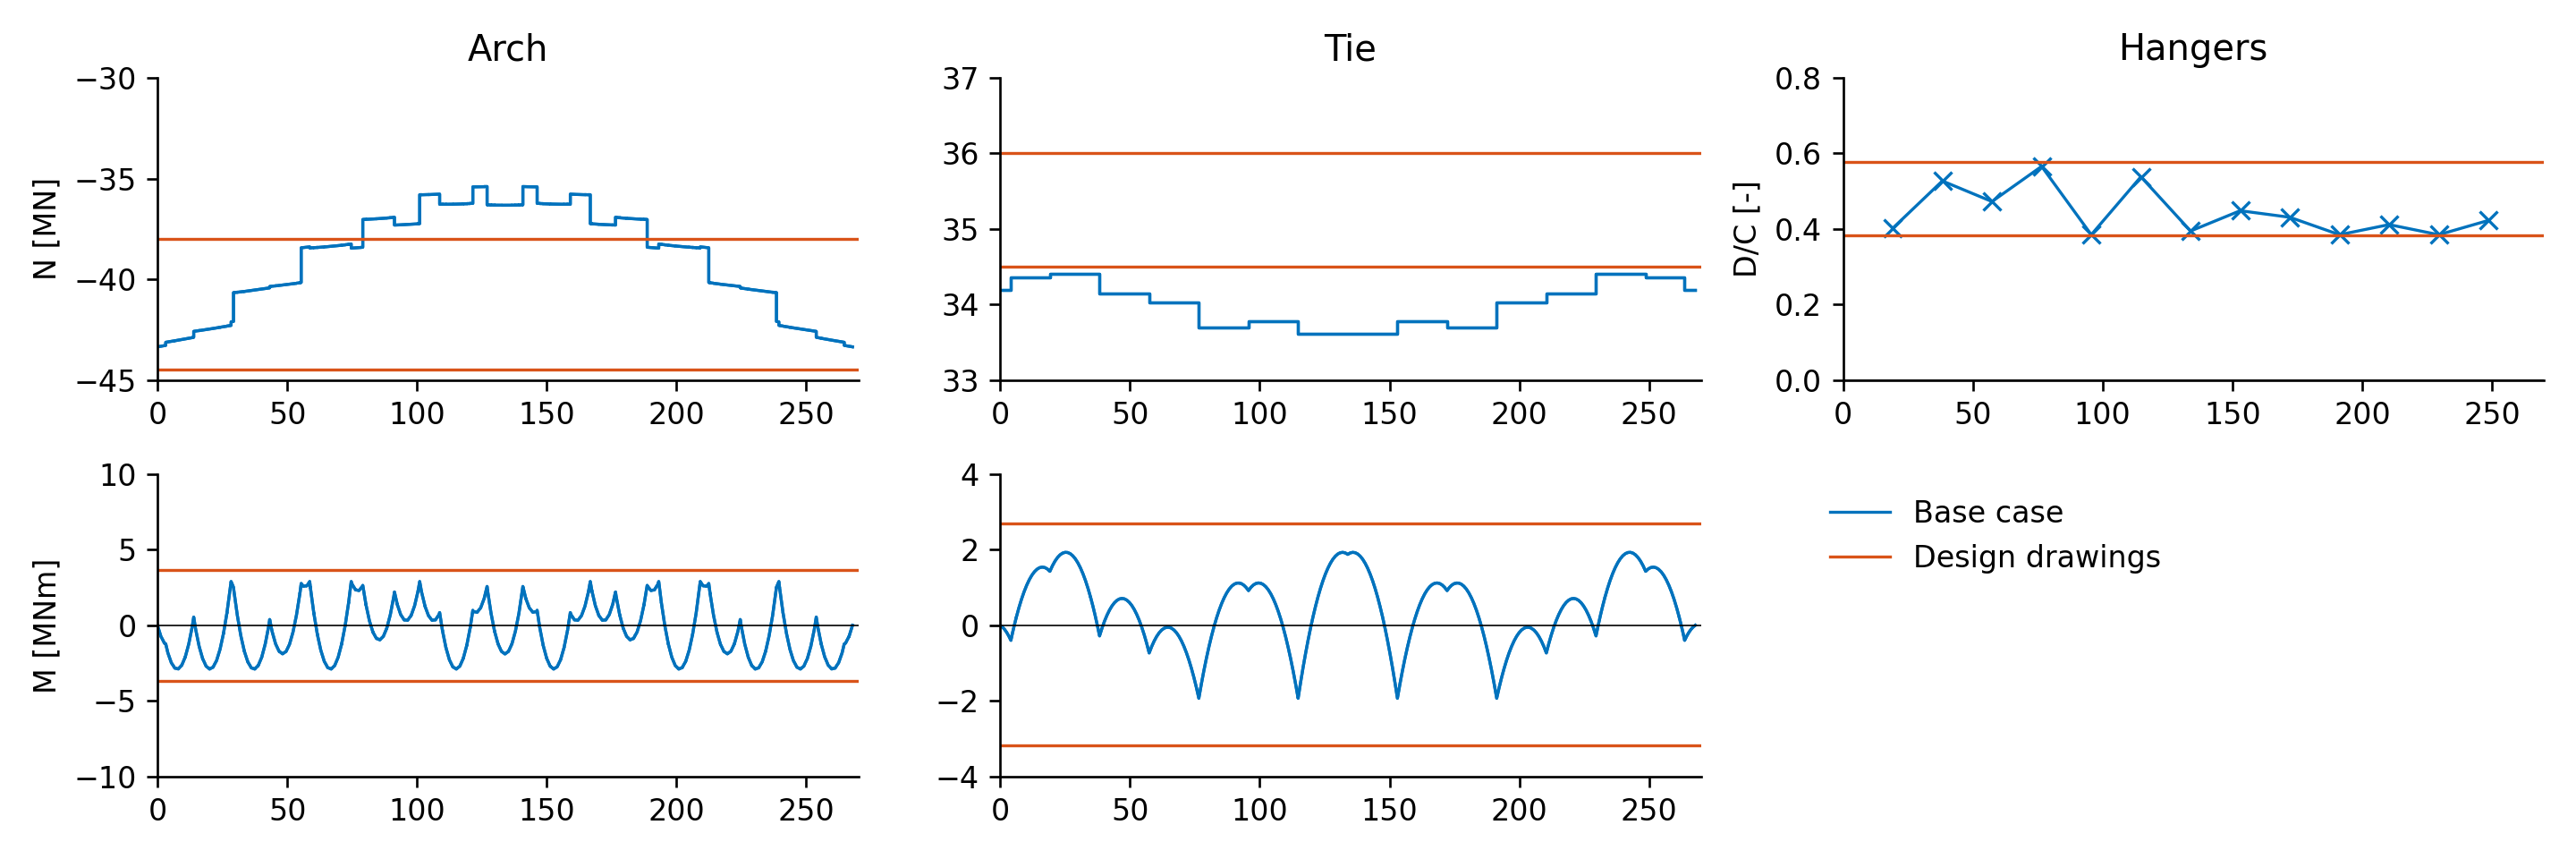
\includegraphics[width=\textwidth]{calculations/Base case/Permanent state.png}
    \caption{Permanent internal forces of the base case and reference values from the drawings}
    \label{fig:base_case_permanent}
\end{figure}

The moment distributions in the arch and the tie, as well as the normal forces in the hangers, match the design drawings very well. Only for the normal force in the arch rib and the tie girder an offset of \SI{2}{MN} can be observed. This difference is probably due to underestimating the weight of the bridge and because of its simplified assignment to the beam elements. However, overall the obtained internal force distribution matches the design drawings sufficiently well. Further, It can be concluded, that for a fixed arch shape the simultaneous arch and tie moment optimisation yields adequate results. Another comparison is drawn between the effects under characteristic live loads. As there are countless live load combinations, which are to be accounted for, it makes sense to look at the entire range of possible internal forces. They are shown in Fig. \ref{fig:base_case_live} by the two blue lines representing the lower and the upper limit. These ranges are compared to the values specified in the design verifications of the design drawings.

\begin{figure}[H]
    \centering
    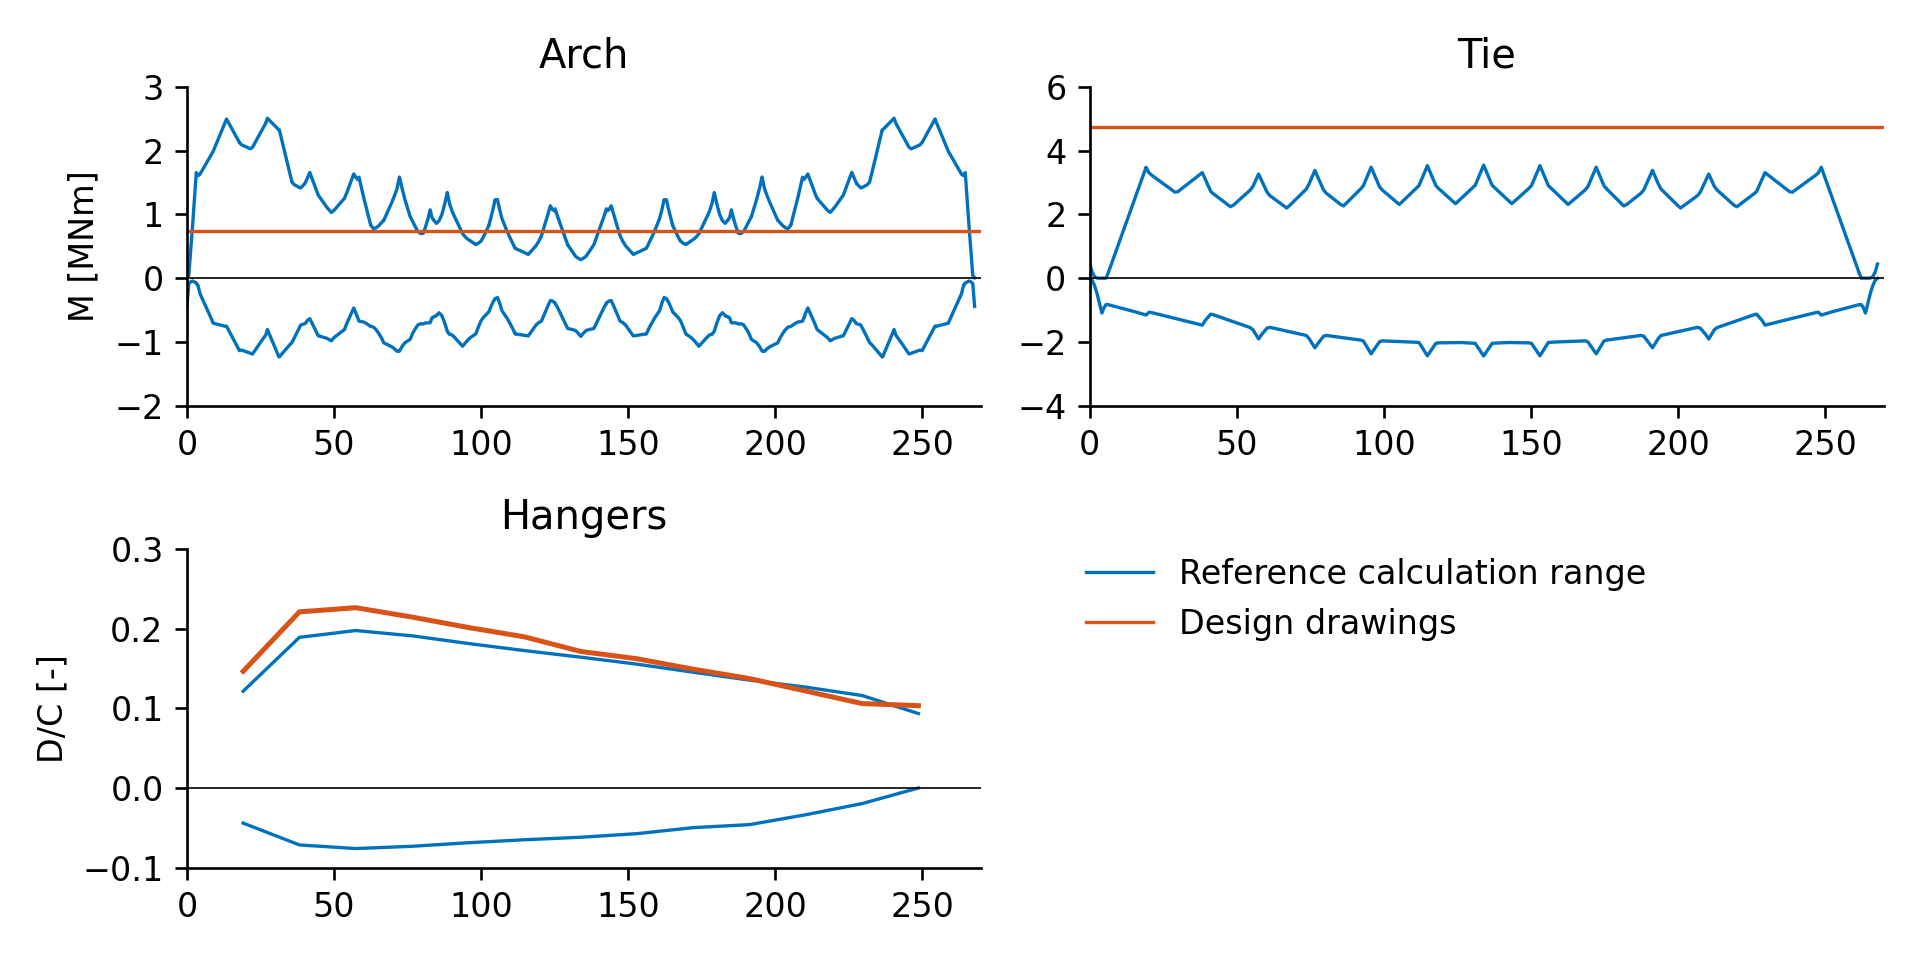
\includegraphics[width=0.8\textwidth]{calculations/Base case/Live load.png}
    \caption{Range of internal forces effects under live loading}
    \label{fig:base_case_live}
\end{figure}

The moment distribution in the arch shows a a significant offset to the value given in the design drawings. However, it is impossible that this value represents the maximum moment under live loading, considering the given hanger forces. Therefore, this difference is ignored. The moment distribution in the tie and the hangers' normal forces agree well on the other hand. Apparently, the live loading is only slightly overestimated in the model, which can be seen particularly well in the hangers' demand over capacity ratios. These differences are accepted, as it is not the goal of this Thesis to reproduce the results from the design drawings. Interestingly, in particular, the arch segment near the knuckle is affected by strong bending moments. In the tie girder on the other hand, the range of effects under live loading is well distributed. Apparently, the influence lines for the moments in the tie girder at the different cross-girders roughly follow the same shape. For the hangers, it is the second one from the knuckle connected toward the middle of the arch that undergoes the largest normal force. Towards the other side of the hanger set, the hanger forces decrease. The strongly affected hangers have in common that their inclination is closer to the arch's inclination at their respective connection node. The arch is very stiff on axial loading and comparably weaker on perpendicular forces. Therefore, at the arch nodes, smaller displacements in the hanger's direction are expected for the first hangers of the considered hanger set, explaining their higher normal forces. Only the first hanger does not follow this rule, which is explained by its smaller area of influence due to the nearby knuckle. \medskip

The resulting demand over capacity ratios for all segments and limit states are presented in Table \ref{tab:dc_base_case}. Considering the strength limit states, wind exposure is governing for the segment close to the knuckle for both the arch and the tie. For the segment in the field, as well as for the hangers, it is the vehicular load which poses the highest demand. The limit state for high dead-to-live load ratios is not decisive for any segment. A comparison to the ratios found in the design drawings, presented in Table \ref{tab:dc_drawings}, shows that this is not the case for the final design. The underestimation of the demand of the strength-IV limit state is probably due to a general underestimation of the weight, which has already been seen for the permanent effects. Nonetheless, the strength limit states agree well with the verifications found in the design drawings, even though slightly underestimated. For cable loss and replacement on the other hand, the demands predicted by the considered model are overestimated. Besides the higher dynamic amplification factors of 1.75, this is due to the modelling of a single arch plane, which does not take into account the other undamaged arch plane. Nevertheless, the results are within an acceptable range. For the tie fracture extreme event, which is considered in a simplistic manner, demands near 1.00 result. This agrees with the design drawings, in which it is only noted that the tie fracture governed the design of the tie girder. For the comparative investigations in this Thesis the simplistic verification is adequate, as the tendencies can be modelled sufficiently accurate.

\begin{table}
    \centering
    \caption{Demand over capacity ratios of the base case}
    \label{tab:dc_base_case}
    \input{calculations/Base case/dc table.txt}
\end{table}

\begin{table}[H]
    \centering
    \caption{Demand over capacity ratios of the final design}
    \label{tab:dc_drawings}
    \begin{tabular}{lccccccc}
    \toprule
    Segment & \multicolumn{7}{c}{Demand / Capacity} \\
     & S-I & S-III & S-IV & Replacement & Loss & Fracture & Fatigue\\ \midrule 
    Arch 1 & - & \textbf{1.00} & - & - & 0.85 & -  & - \\ 
    Arch 2 & - & - & 0.99 & - & \textbf{1.00} & -  & - \\ 
    Arch 3 &  - & - & 0.83 & - & \textbf{0.97} & -  & - \\ 
    Tie 1 & - & 0.69 & - & - & 0.61 & $\sim$\textbf{1.00} & - \\ 
    Tie 2 & 0.68 & - & - & - & 0.88 & $\sim$\textbf{1.00} & - \\ 
    Tie 3 & 0.63 & - & - & - & 0.76 & $\sim$\textbf{1.00} & - \\ 
    Hangers & 0.91 & 0.77 & 0.75 & - & 0.74 & -  & -\\ 
    \bottomrule
\end{tabular}

\end{table}

\newpage
\section{Arch shape} \label{sec:arch_shape}
Traditionally, mainly the circle and the parabola have been used as arch shapes. The parabola has served well as a shape for traditional tied-arch bridges with vertical hangers. In this case, the vertical hanger forces on the arch are evenly distributed and the respective thrust line matches the parabola. For network tied-arch bridges, circular shapes have been considered suitable for radial arrangements. In this case, uniform hanger forces cause an approximately radial loading on the arch, which results in a circular thrust line. For a rise to span ratio of 0.2, the two shapes diverge by at most 0.8\% of the span. While this differences might seem negligible on a drawing, the impact of this difference on the arch's moment distribution is significant, as it is bigger than its usual cross-section height. In this section, the arch shape is first investigated individually as it affects the investigation of all other variables. The extreme events of cable loss are disregarded for in this investigation, because their impact depends much more on the hanger arrangement than on the arch shape.
Multiple approaches to determine the arch shape have been introduced in Section \ref{sec:met_arch}. All of them are linked to the thrust line, which is approximately the most efficient shape. The following four arch shapes are compared in this investigation.
\begin{enumerate}
    \item Thrust line: This shape is obtained numerically as the thrust line for the hanger forces, which are obtained from a tie moment optimisation. The respective hanger forces are uniform at $N_p=\SI{1.8}{MN}$ which corresponds to 28\% of their characteristic resistance.
    \item Polynomial thrust line approximation: The above thrust line is approximated by a quartic function. The quartic function is described by Eq. \eqref{eq:polynomial_shape} using the shape parameter $b$. This parameter is obtained by a least squares approximation. It fulfills the conditions $y(0)=r$ and $y(s/2)=0$
    \begin{equation}
        y(x)=r \cdot \left(1 - b \cdot \left(\frac{2\,x}{s}\right)^2 - (1-b) \left(\frac{2\,x}{s}\right)^4 \right)
        \label{eq:polynomial_shape}
    \end{equation}
    \item Spline thrust line approximation: As a second approximation of the thrust line a cubic spline defined by the respective arch-hanger connection nodes is used. These nodes are therefore represented at their exact location.
    \item Thrust line of continuous hanger arrangement: This shape is the thrust line of the hypothetical continuous hanger arrangement, which was introduced in Section [].
\end{enumerate}

To make their differences visible, the respective deviations to the parabolic shape are shown in Fig. \ref{fig:arch_shapes_13}. Also a circular arch is shown to put the results into perspective.

\begin{figure}[H]
    \centering
    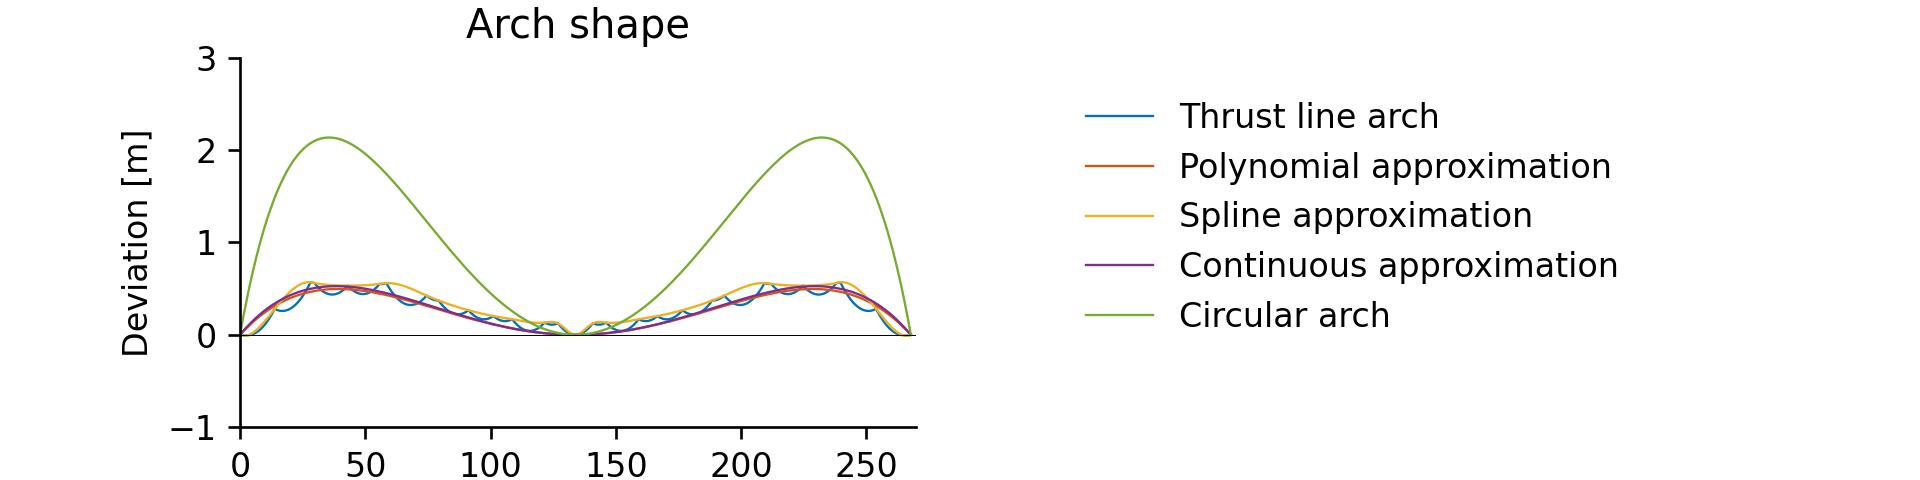
\includegraphics[trim={1cm 0 3cm 0},clip, width=0.76\textwidth]{calculations/arch shape/arch_shapes_13.png}
    \caption{Deviation of arch shapes to the parabola}
    \label{fig:arch_shapes_13}
\end{figure}

In the range between the circular and the parabolic shape, the thrust line tends slightly to the parabolic side. All three approximations seem to fit the thrust line reasonably well. But to investigate the impacts of the remain deviations from the thrust line, the corresponding permanent moment distribution is presented in Fig. \ref{fig:arch_permanent_moments_13}. Further, from the similarity between the polynomial and the continuous approximation, it can be concluded, that if the hanger arrangement is dense enough, a quartic function can yield an appropriate arch shape for this hanger arrangement pattern. 

\begin{figure}[H]
    \centering
    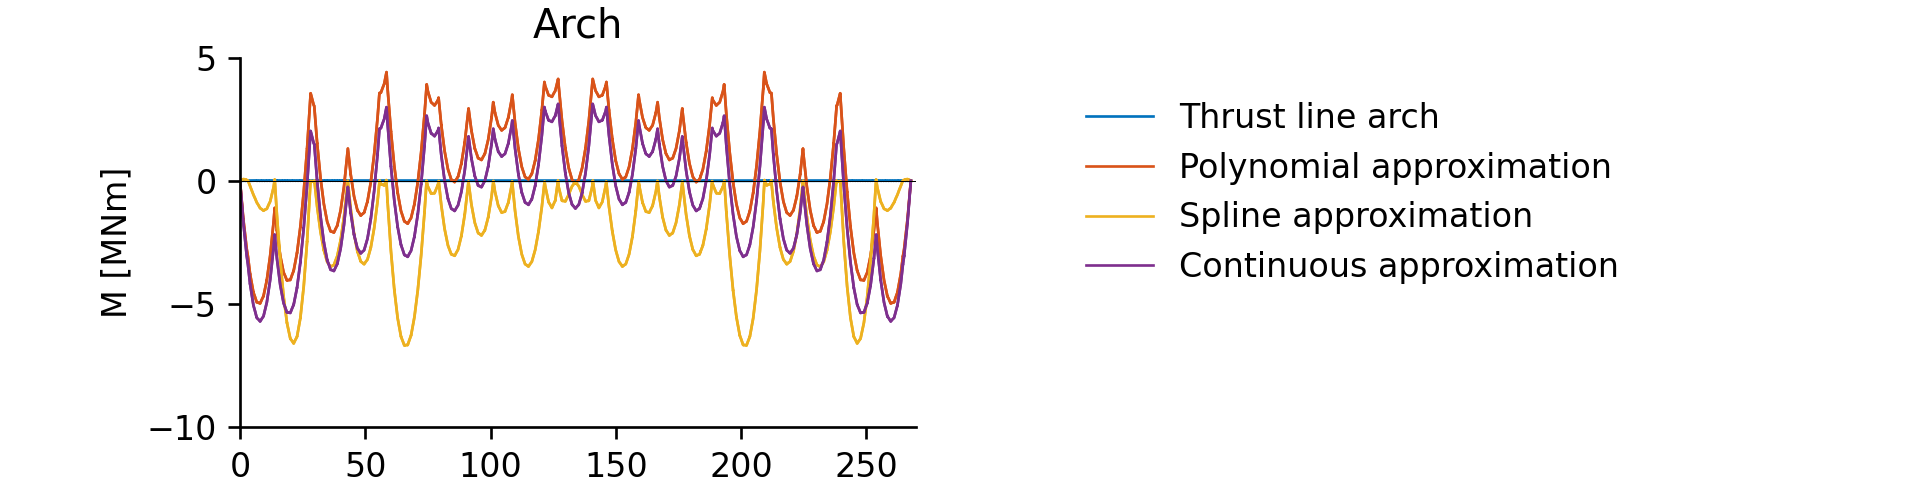
\includegraphics[trim={1cm 0 3cm 0},clip, width=0.76\textwidth]{calculations/arch shape/permanent state_13.png}
    \caption{Permanent arch moment distributions depending on arch shape}
    \label{fig:arch_permanent_moments_13}
\end{figure}

Despite the apparent match of the arch shapes, significant bending moments result in each of the three approximations. The spline approximation's moment distribution is strictly negative, which relies on the characteristic that a spline lies above the approximately linear thrust line and only matches it at the connection nodes. It is particularly interesting, that all approximations feature a similar parabolic moment distribution between the arch-hanger connection nodes. While these moment distributions resulting for the approximated shapes are certainly considerable, it is practically infeasible to find a simple shape matching the arch thrust line. Any shape with an approximately constant radius $R$ results in a certain deviation from the thrust line and the corresponding moment deviation $\Delta M$. This deviation can be approximated depending on the distance between two hanger points $d$ and the arch's normal force $N$ according to Equation \eqref{eq:moment_deviation}.

\begin{equation}
    \Delta M=-\left(R-\sqrt{R^2-\left(d/2\right)^2}\right) \cdot N
    \label{eq:moment_deviation}
\end{equation}

For the Blennerhassett Island Bridge, these variables roughly correspond to $R=\SI{194}{m}$, $d=\SI{17}{m}$ and $N=\SI{40}{MN}$. Equation \eqref{eq:moment_deviation} yields a moment deviation of $\Delta M=\SI{7.5}{MNm}$ coming close to the value observed in Fig. \ref{fig:arch_permanent_moments_13}. From the analytical form of Equation \eqref{eq:moment_deviation} it can further be concluded, that a reduction of the hanger node spacing has a more than proportional impact on the bending moment deviation. To put these deviations into the context of the design verifications, the demand over capacity ratios resulting in the arch are shown in Table \ref{tab:arch_shape_dc_13} along with the decisive limit state.

\begin{table}[H]
    \centering
    \caption{Arch design verifications for different arch shapes}
    \label{tab:arch_shape_dc_13}
    \input{calculations/arch shape/dc_comparison_13.txt}
\end{table}

The deviations from the thrust line of the considered arch shapes increase the demand over capacity ratios by 0.06 on average. This difference is not critical for the initial design, but it offers some potential for optimisation. Further, it should be noted that also the exact thrust line is not the most efficient arch shape. In the strength limit state for vehicular use, the arch is affected by stronger positive bending moments than negative ones, as shown in Fig. \ref{fig:arch_shape_strength_1}. Therefore, a certain upward deviation from the thrust line and the resulting negative bending moment can prove beneficial to the verifications. This potential was estimated by evaluating the difference of the maximum and minimum bending moments in the decisive limit state and comparing it to the resistance. The comparison yielded possible reductions for the three segments between 0.01 and 0.03.

\begin{figure}[H]
    \centering
    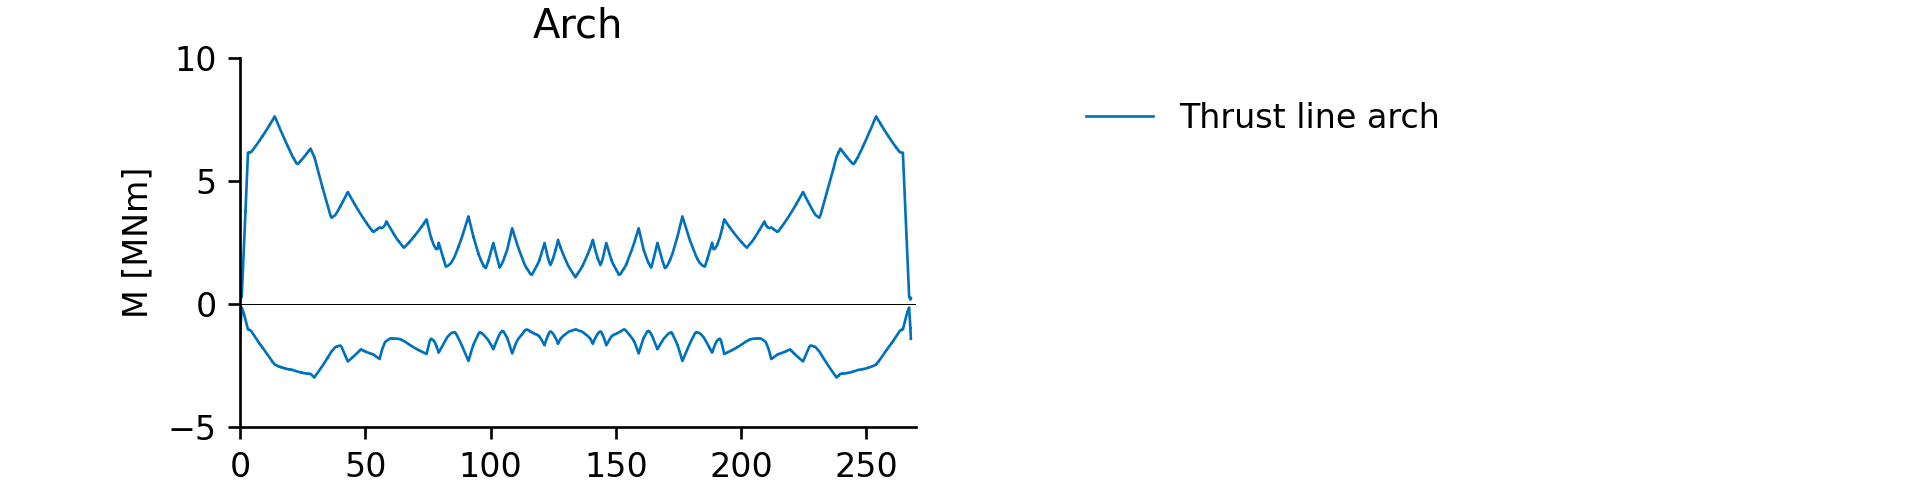
\includegraphics[trim={1cm 0 3cm 0},clip, width=0.76\textwidth]{calculations/arch shape/strength-I_13.png}
    \caption{Range of moments in the strength-I limit state}
    \label{fig:arch_shape_strength_1}
\end{figure}

Ultimately, the influence of the hanger density on the arch shape is investigated. It was concluded from Equation \eqref{eq:moment_deviation}, that by reducing the distances between the hangers an over-proportional reduction in the permanent moment distribution results. Therefore, a similar calculation of the four arch shapes with 26 hangers per set was conducted. The resulting arch shapes are presented in Fig. \ref{fig:arch_shapes_26}.

\begin{figure}[H]
    \centering
    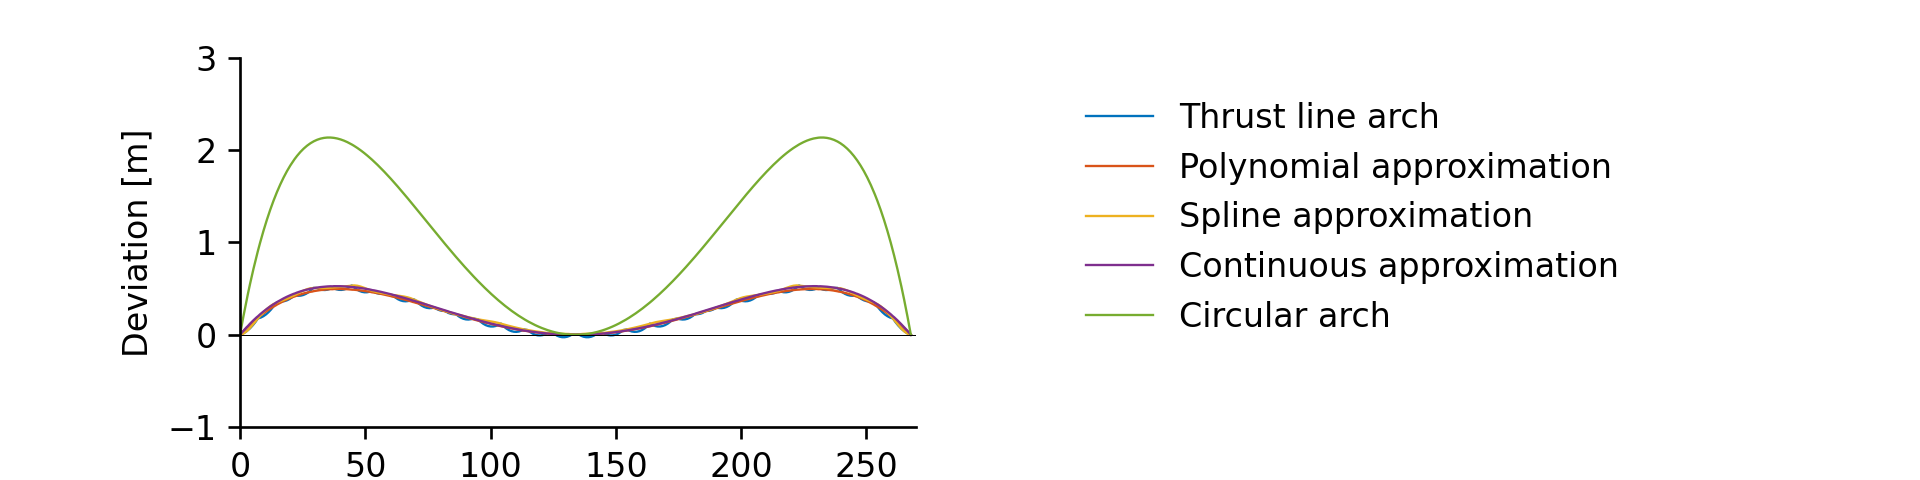
\includegraphics[trim={1cm 0 3cm 0},clip, width=0.76\textwidth]{calculations/arch shape/arch_shapes_26.png}
    \caption{Deviation of arch shapes from parabolic shape (26 hangers)}
    \label{fig:arch_shapes_26}
\end{figure}

If the amount of hangers is large enough, all considered approximations yield suitable arch shapes. The impact of the remaining deviation from the thrust line on the design verifications is negligible, as can be seen in the uniform demand over capacity ratios presented in Table \ref{tab:arch_shape_dc_26}. For the initial design, especially the continuous approximation presents a promising arch shape, as it does not involve a specific thrust line calculation. However, for sparse hanger arrangements, a more accurate modelling of the thrust line, involving the characteristic kinks, might be inevitable for the arch shape.

\begin{table}[H]
    \centering
    \input{calculations/arch shape/dc_comparison_26.txt}
    \caption{Arch design verifications (26 hangers)}
    \label{tab:arch_shape_dc_26}
\end{table}


\newpage
\section{Hanger density}
A denser hanger arrangement provides multiple benefits. As seen in the previous chapter, the shape deviation moments are reduced through the corresponding reduction of the distances between the hangers' anchorages. Further, the effects in the extreme event of cable loss are significantly lowered, as the hanger forces are reduced with the increase of hangers. Also the impaired structural system loses less of its essential stiffness and undergoes additionally lower effects therefore. However, the challenging task is to find an appropriate self-equilibrium stress state for structural systems in which the locations of the floor beams and the hangers do not coincide on the tie girder. 
In this investigation, this challenge is tackled by tie moment optimisation method. It allows finding the permanent hanger forces within a certain range, minimising the resulting moment distribution in the tie girder. This range is set between 25\% and 40\% of the hangers' characteristic capacity.  Four bridges are analysed featuring 13, 20, 26 or 27 hangers per set and a constant number of 13 floor beams. The arch shapes are defined as the quartic polynomial approximation of the thrust line. The model featuring 26 hangers is shown in Fig. \ref{fig:structure_26}. The spacing between the knuckle and the first hanger is slightly increased so there is an equally spaced pair of hangers around every floor beam. While the arrangement appears dense, the hanger spacing on the tie girder is still around \SI{10}{m} representing a rather high value for modern network tied-arch bridges.

\begin{figure}[H]
    \centering
    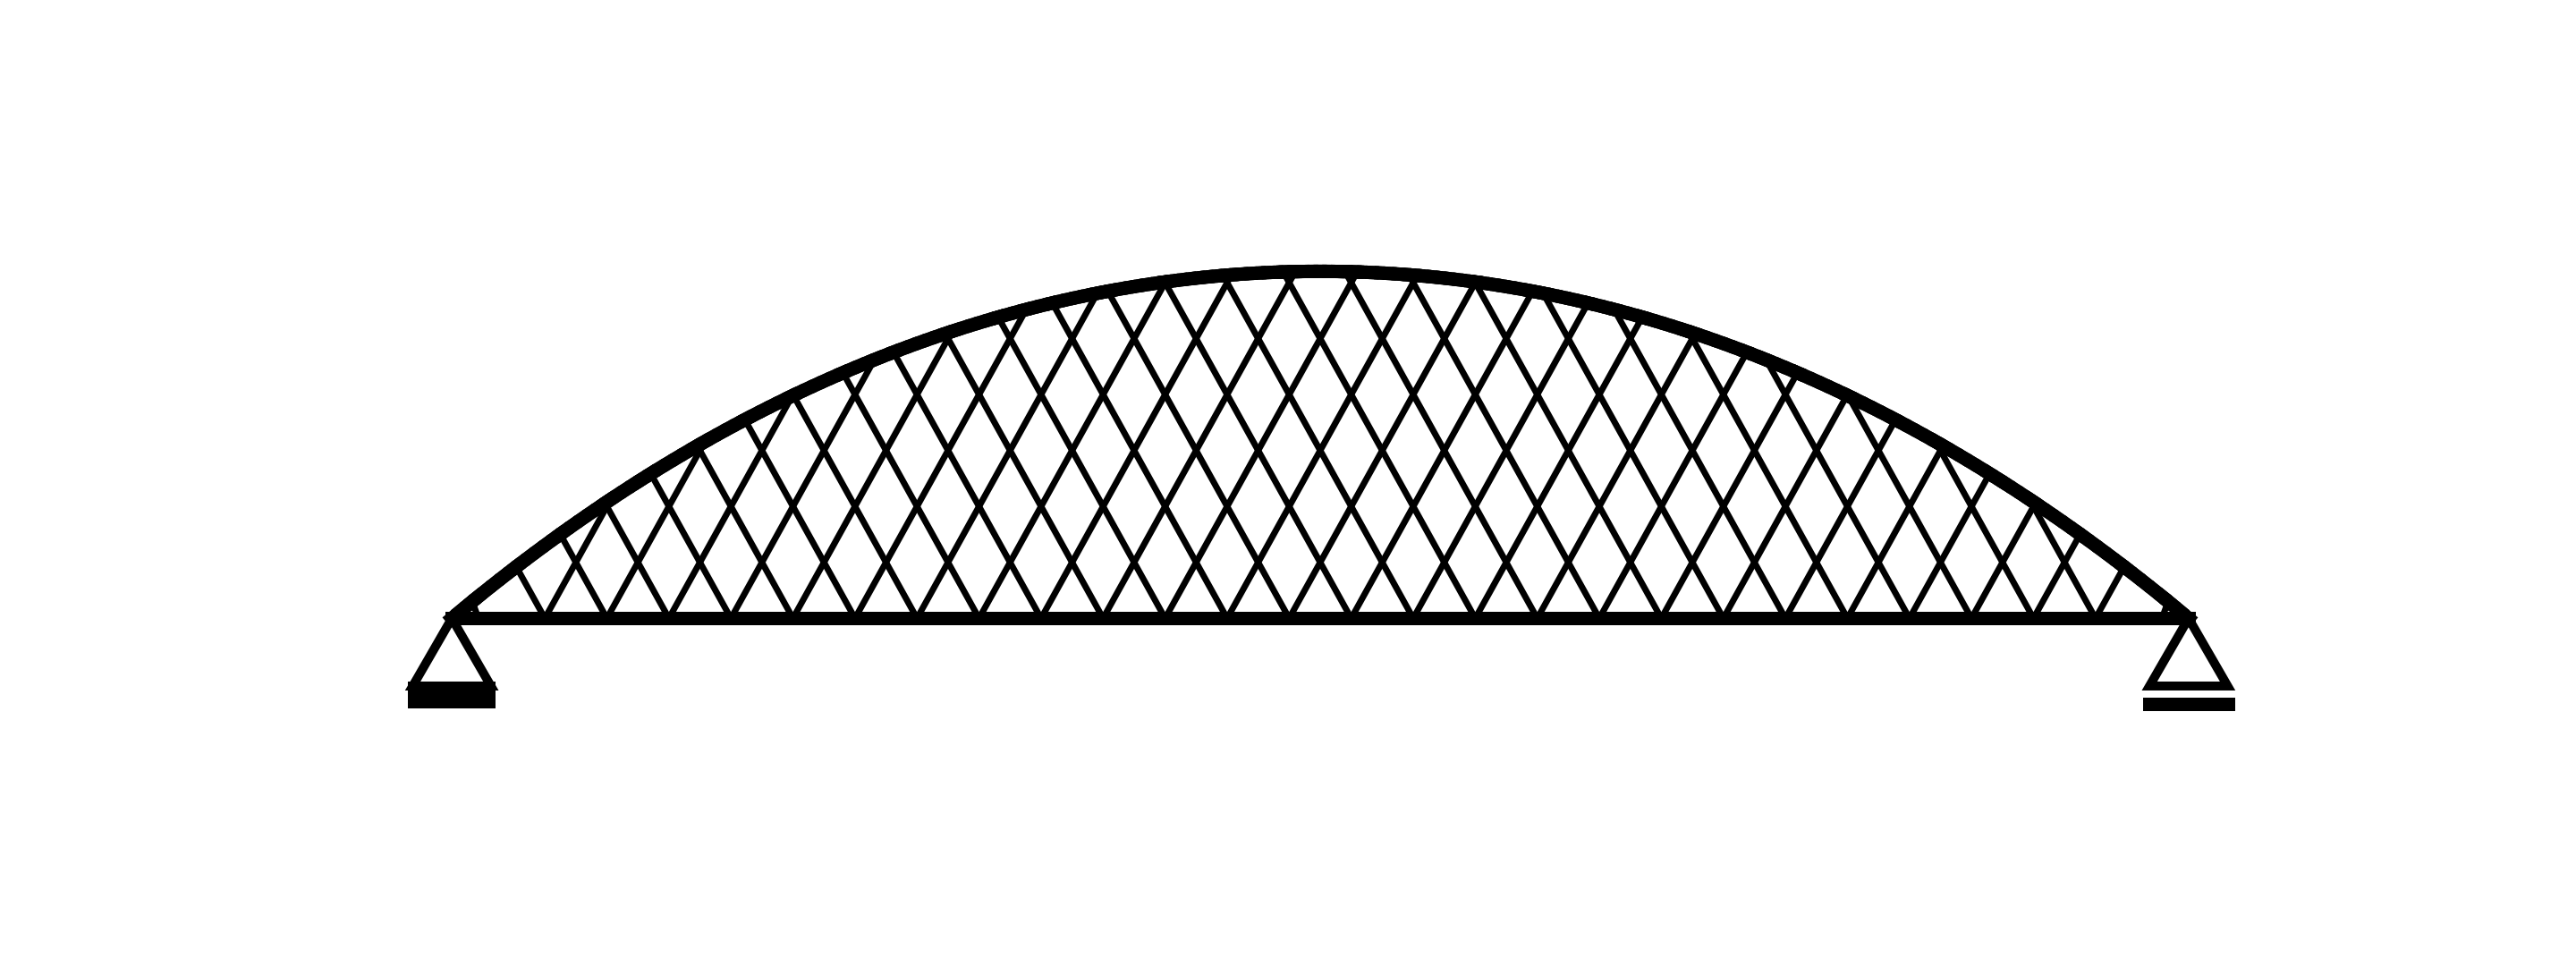
\includegraphics[trim={0 1cm 0 1cm},clip, width=0.65\textwidth]{calculations/hanger amount comparison/structure_26.png}
    \caption{Structural model of a dense hanger arrangement with 26 hangers per set}
    \label{fig:structure_26}
\end{figure}

The optimised effects under permanent loads are shown in Fig \ref{fig:hd_permanent}. As predicted by the investigation of the arch shape, the bending moments in the arch are lowered for an increased hanger density. However, in the knuckle region of the arch the significant bending moments are retained for the dense arrangements. They are due to the tie moment optimisation method assigning significant supernumerary moments to the knuckle. The quartic polynomial approximation is not able to match the corresponding thrust line. The permanent hanger forces are no longer constant for the models with 20 and 27 hangers, as the hangers near the floor beams carry the majority of the forces. At the same time a strong bending moment distribution in the tie is inevitable. The model featuring 26 hangers seems slightly more suitable as it is able to retain constant hanger forces and also a slightly lower tie moment distribution.

\begin{figure}[H]
    \centering
    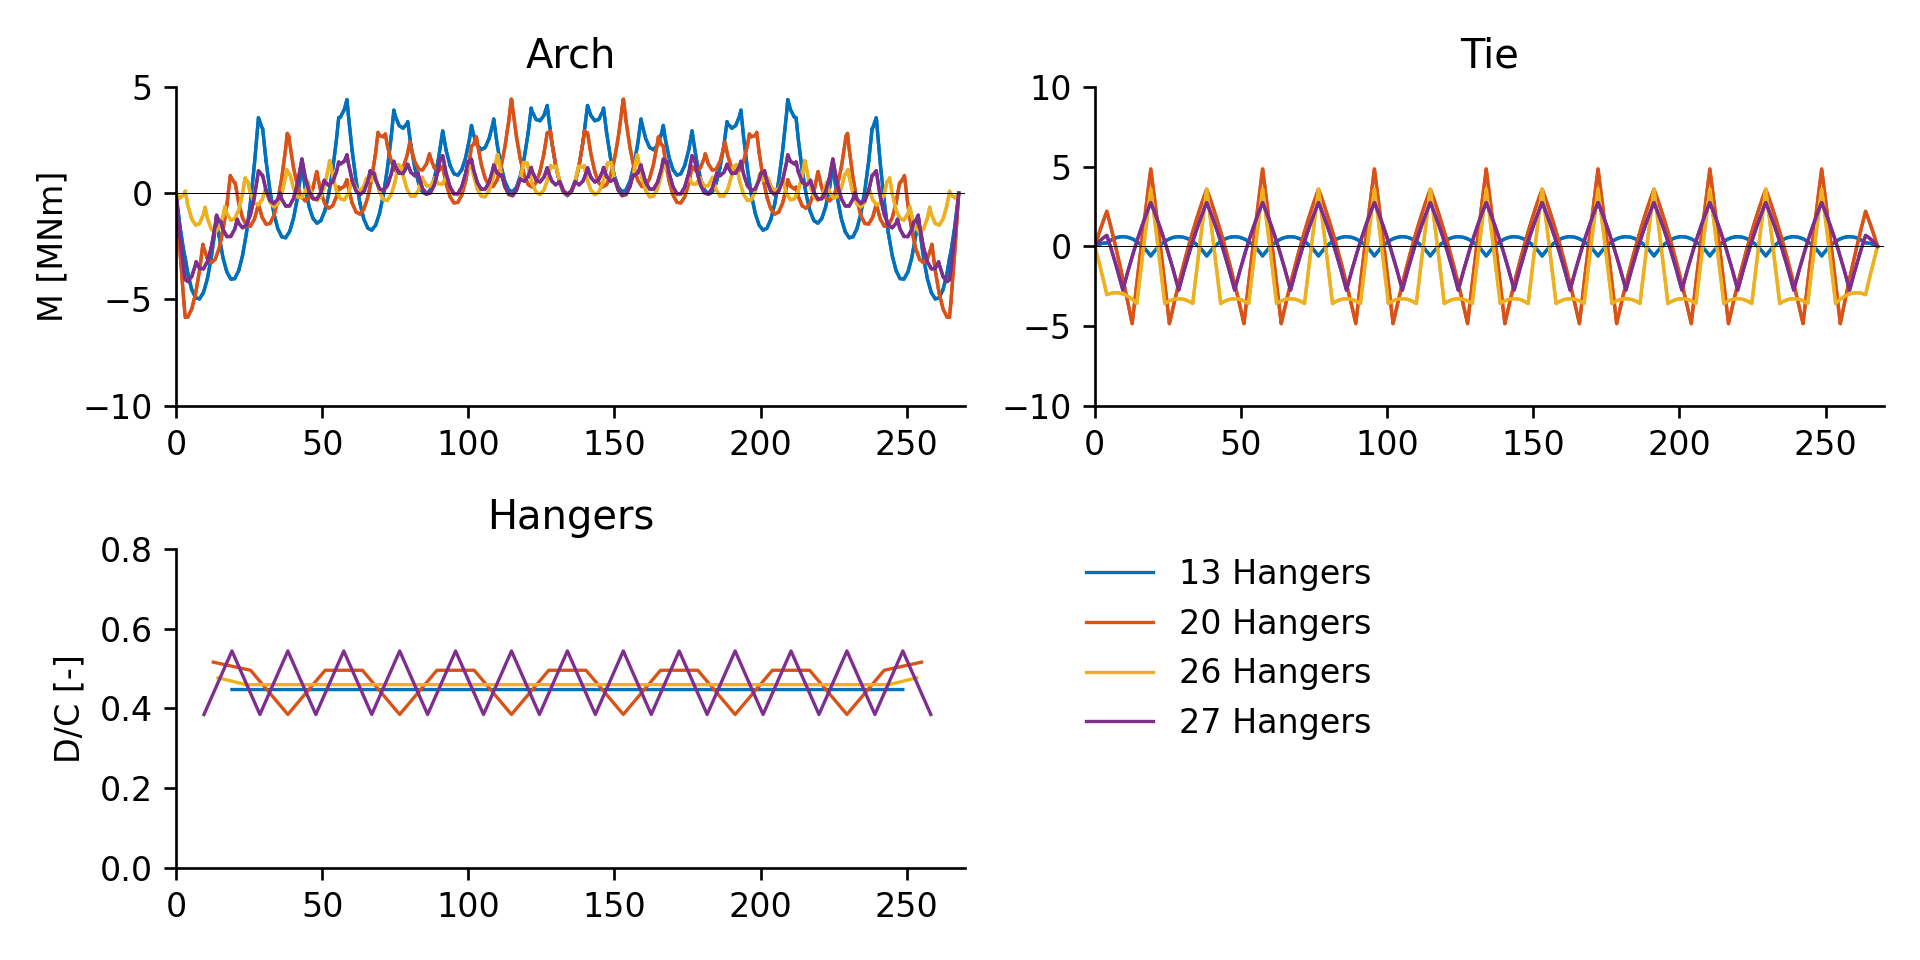
\includegraphics[width=0.75\textwidth]{calculations/hanger amount comparison/permanent state.png}
    \caption{Optimised permanent effects for different hanger densities}
    \label{fig:hd_permanent}
\end{figure}

The elastic responses to dead loading are shown in Fig. \ref{fig:hd_elastic_response_dl}.
%On top of the disadvantageous permanent effects, also the elastic response of the modified models to live loading, which are shown in Fig. \ref{fig:hd_live}, seem unfavourable.

\begin{figure}[H]
    \centering
    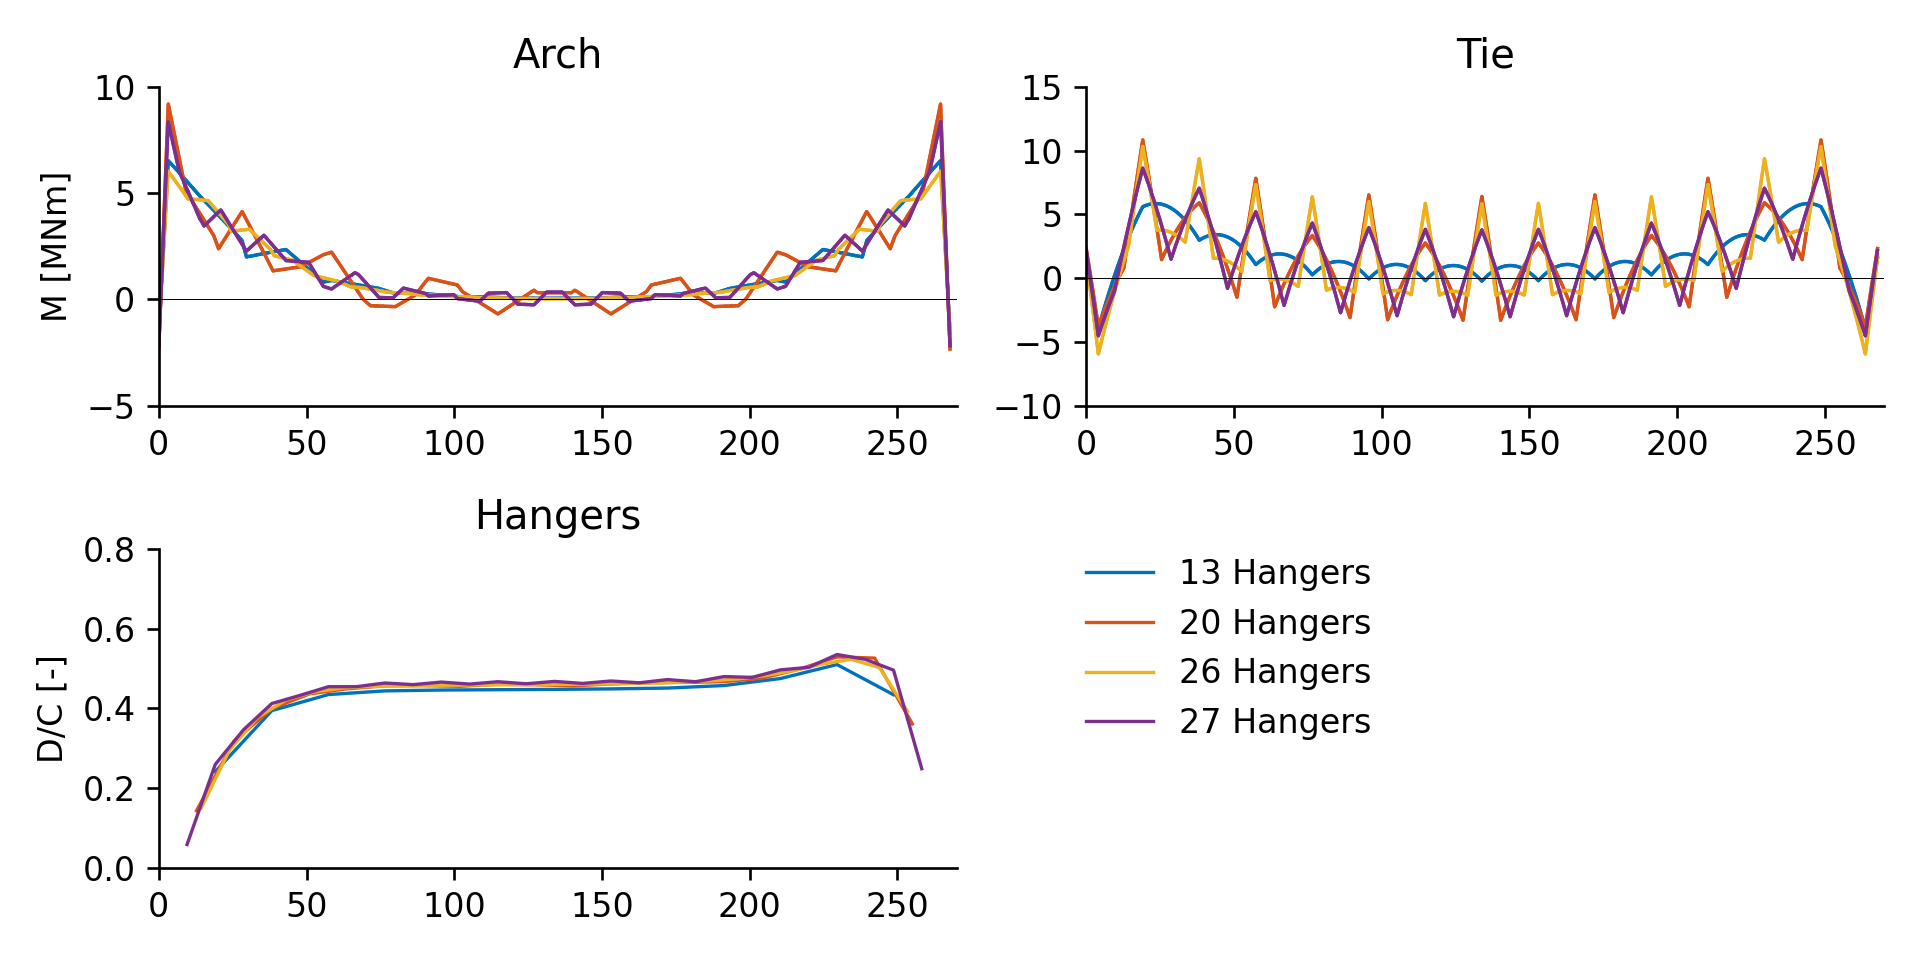
\includegraphics[width=0.8\textwidth]{calculations/hanger amount comparison/dead load.png}
    \caption{Elastic response to dead loading for different hanger densities}
    \label{fig:hd_elastic_response_dl}
\end{figure}

While these effects are already included in the permanent effects, they are still relevant for the design verifications as they are increased or decreased therefor. While the response of the arch and the hangers remains approximately identical, the tie is again affected by stronger bending moments in the denser models. This characteristic is accentuated by the range of tie moments relevant for the tie fracture extreme event, presented in Fig. \ref{fig:hd_tie_fracture}.

\begin{figure}[H]
    \centering
    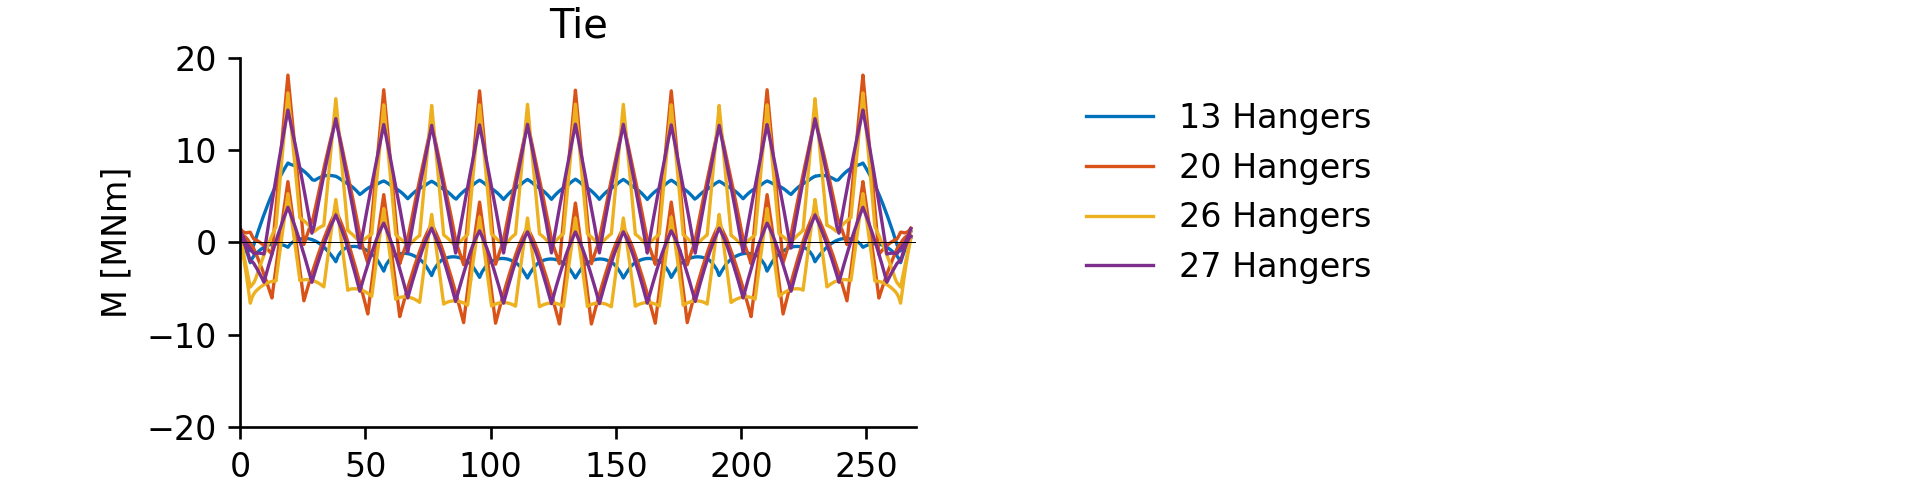
\includegraphics[trim={0 0 3cm 0},clip, width=0.8\textwidth]{calculations/hanger amount comparison/tie fracture.png}
    \caption{Range of tie bending moment for tie fracture extreme event}
    \label{fig:hd_tie_fracture}
\end{figure}

The previously rather uniform moments became particularly peaky. The corresponding design verification in the tie is thereby significantly impaired, as show in Table \ref{tab:hd_dc}. An optimisation of the hanger density itself, therefore renders no potential for optimisation, even though the cable loss extreme event improves as expected.

\begin{table}[H]
    \centering
    \caption{Design verifications for different hanger densities}
    \label{tab:hd_dc}
    \resizebox{0.85\columnwidth}{!}{%
    \input{calculations/hanger amount comparison/dc_comparison.txt}
    }
\end{table}


\section{Floor beam density}
It was seen in the previous chapter, that it is impossible to obtain an optimised design with more hangers per set than floor beams. To facilitate the design verifications in the extreme event of cable loss, a denser hanger arrangement has to be paired with a higher floor beam density. It seems a particularly reasonable step, as the Blennerhassett Island Bridge holds the record for hanger spacing on the tie girder at \SI{20}{m}. This was only feasible as the extreme event of floor beam loss was not considered in the design. However, there are other causes to investigate the floor beam and hanger density. Besides the previously mentioned improved behaviour under cable loss and smaller deviations of the arch from the thrust line, a general more continuous transfer of loads might be beneficial. \medskip

Theoretically, an adapted floor beam spacing changes the entire deck system and its weight. However, the deck is not subject to this investigation and it is therefore assumed, that the total weight of the deck system and the floor beams is constant and independent of the floor beam spacing. Four models with different floor beam and hanger densities are investigated in this Section. Besides the final design with 13 floor beams, models with 10, 20 and 27 floor beams are investigated. As an advantage for the sparse model with 10 floor beams, the actual thrust line is assumed as the arch shape. For the other models, the thrust line is approximated by the quartic polynomial. The respective permanent effects are shown in Fig. \ref{fig:fb_permanent}.

\begin{figure}[H]
    \centering
    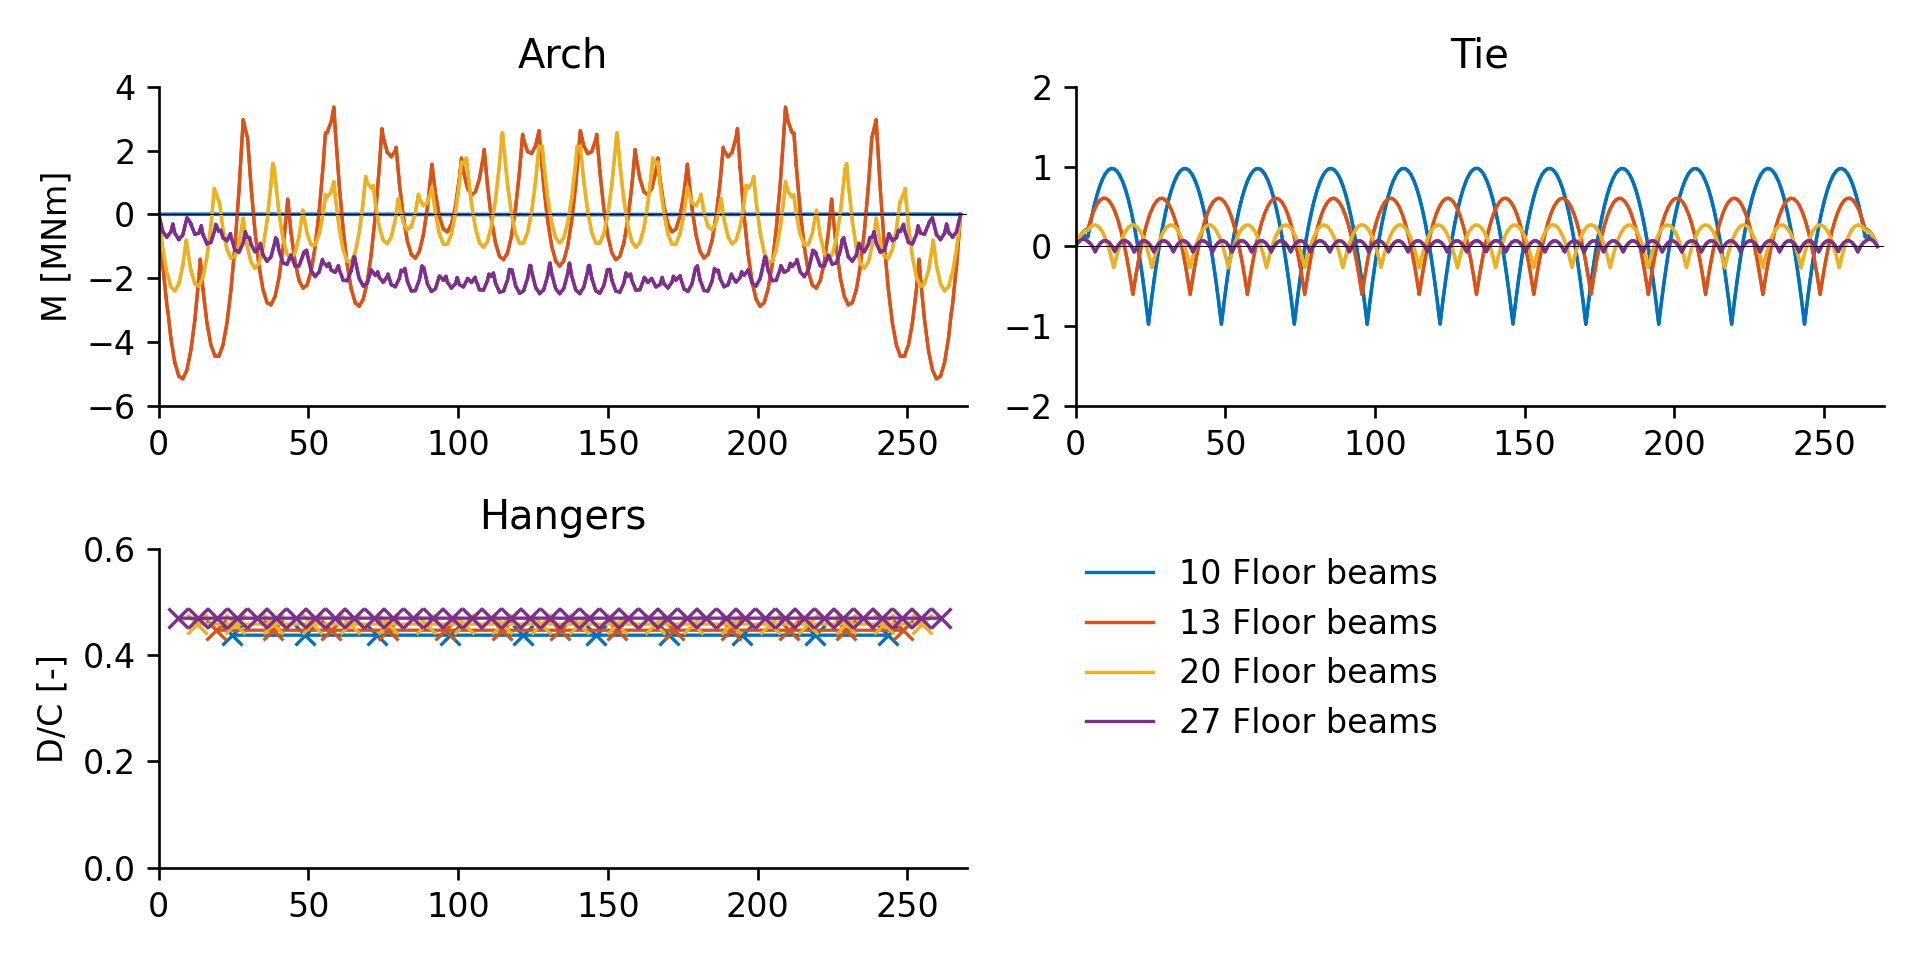
\includegraphics[width=0.8\textwidth]{calculations/floor beam comparison/permanent state.png}
    \caption{Optimised permanent effects for different floor beam densities}
    \label{fig:fb_permanent}
\end{figure}

All models retain the characteristic permanent effects resulting from the tie optimisation, which are the uniform hanger forces and a uniform tie moment distribution with peaks at $M=\pm\,g_{Tie} \cdot s^2 / 16$. It can be seen, that the hanger forces slightly increase, as less weight of the deck is directly carried by the floor beam at the knuckle. Compared to the other models, the permanent arch moments for 13 floor beams seem to be significant. However, it is known from the investigation of the arch shape, that the moments only lower the demand over capacity ratio by about 0.05. \medskip

In Fig. \ref{fig:fb_live} the elastic response under characteristic live loading is shown. For the hangers, the response is practically unchanged. Only the hangers very close to the knuckle undergo a lower normal force, as the tie girder at the knuckle carries the corresponding load directly to the knuckle. For the tie girder, the moment effects increase with the floor beam density and constitutes a slightly impairing impact on the design verifications. The stronger moments are due to the weaker coupling of the tie and the arch at the floor beams. While the force at the floor beams for the distributed lane load decreases, the force of the design trucks remain the same. They are responsible for the slightly increased hanger forces and bending moments in the tie girder. The moment distribution on the arch rib shows a different tendency. Overall the effects of the models resemble a similar shape. However, for fewer floor beams, certain moment peaks due to the stronger hanger forces become apparent. To put these differences into the context of the design verifications, the resulting demand over capacity ratios are shown in Tab. \ref{tab:fb_dc}.

\begin{figure}
    \centering
    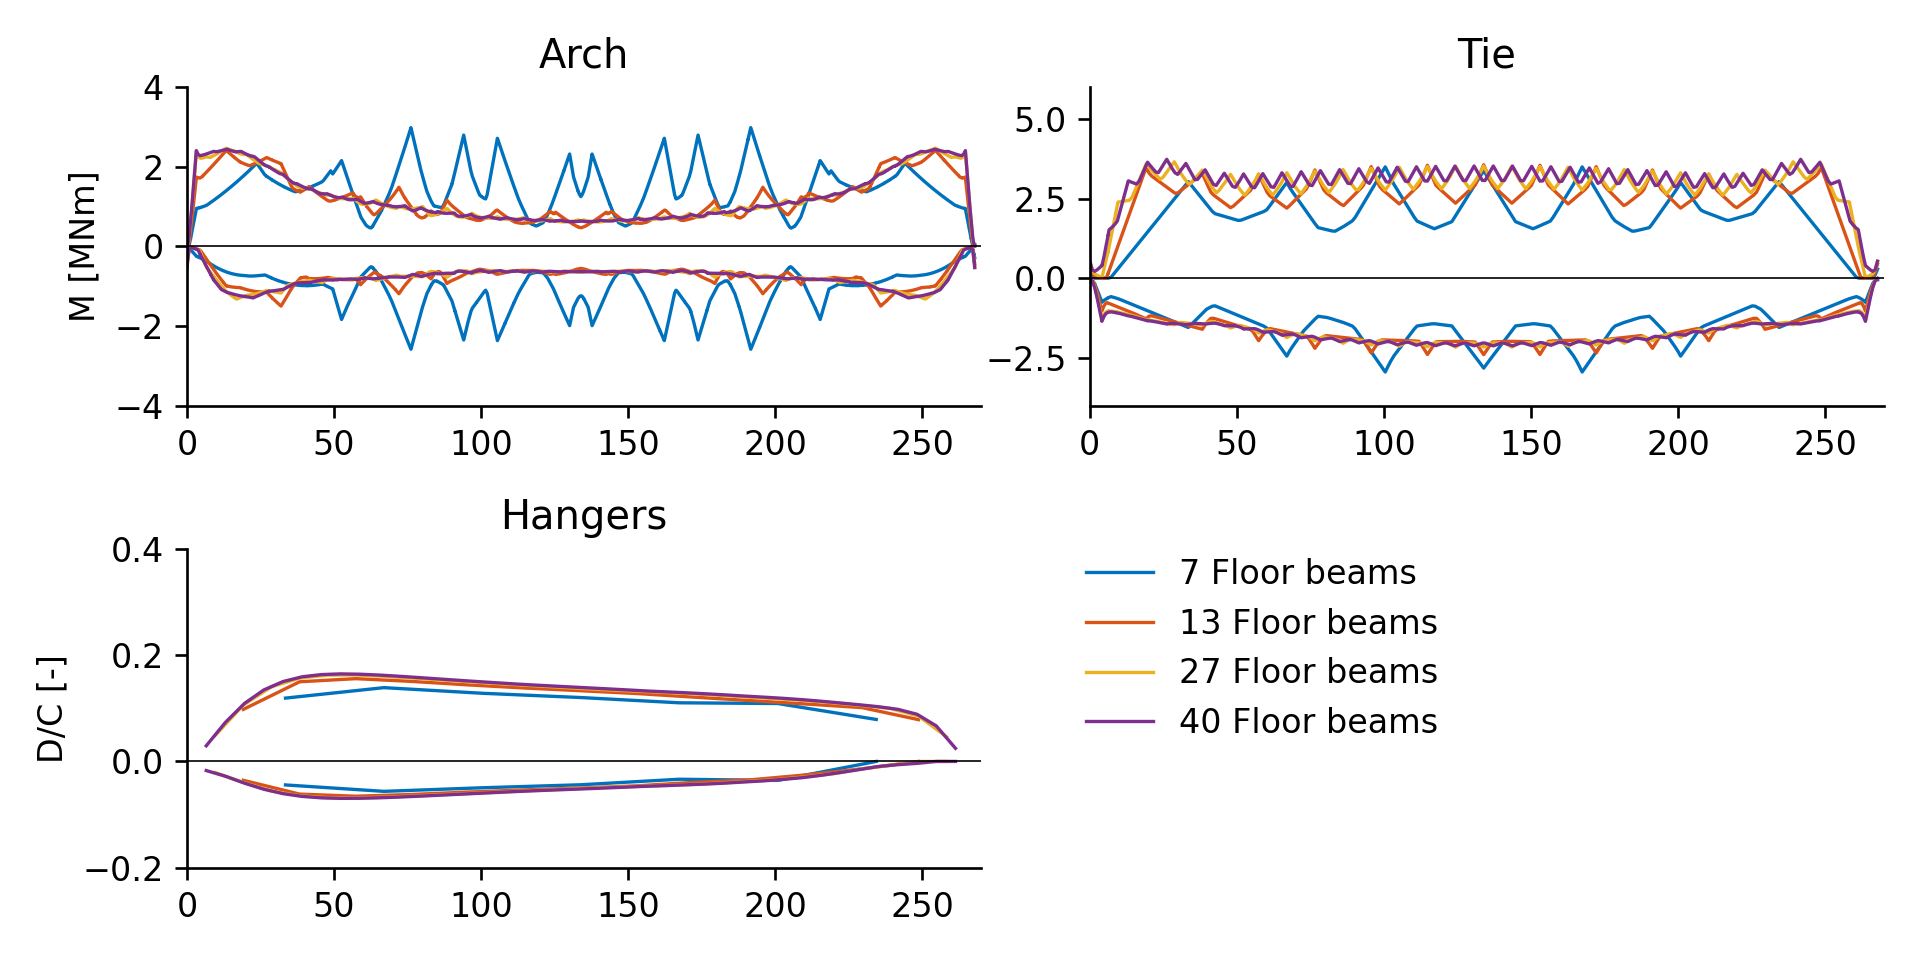
\includegraphics[trim={0 0.4cm 0 0.4cm},clip, width=0.78\textwidth]{calculations/floor beam comparison/live loading.png}
    \caption{Elastic effects under live loading for different floor beam densities}
    \label{fig:fb_live}
\end{figure}

\begin{table}[H]
    \centering
    \resizebox{\columnwidth}{!}{%
    \input{calculations/floor beam comparison/dc comparison.txt}
    }
    \caption{Design verifications for different floor beam densities}
    \label{tab:fb_dc}
\end{table}

The extreme event of cable loss is well controlled by a denser hanger arrangement, as was already observed in the previous chapter. The impacts on the other design verification are comparably small. Both the hangers and the tie girder undergo a decrease of about 0.05 in the demand over capacity ratio. The effect ranges for the strength-I limit state are shown in Fig. \ref{fig:fb_strength} for further details. Considering the arch, 10 floor beams with an optimised shape or 27 floor beams show a well balanced moment distribution. However, also the moments in the other models do not have a decisive influence on the design.

\begin{figure}[H]
    \centering
    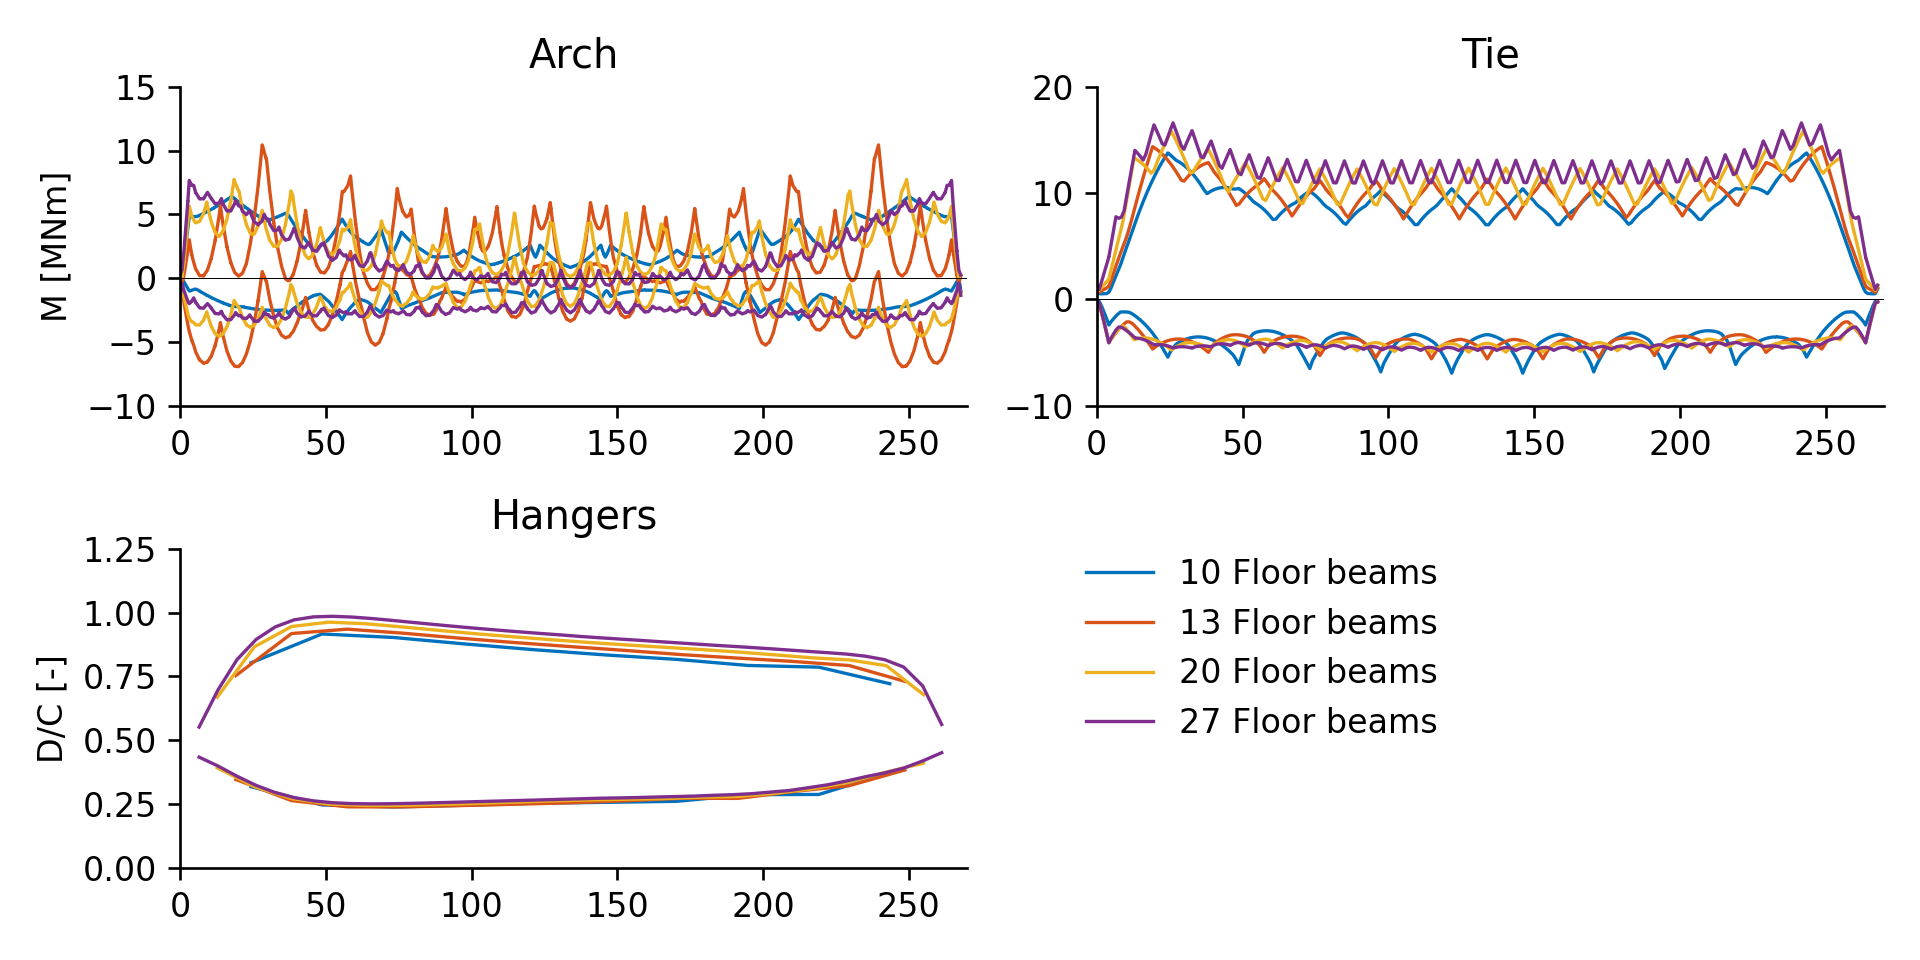
\includegraphics[trim={0 0.4cm 0 0.4cm},clip, width=0.78\textwidth]{calculations/floor beam comparison/strength-I.png}
    \caption{Strength-I effects for different floor beam densities}
    \label{fig:fb_strength}
\end{figure}

[Beschreibung des Kostenverlaufs]

\begin{figure}[H]
    \centering
    \includegraphics[width=0.7\textwidth]{calculations/floor beam comparison/cost comparison.png}
    \caption{Estimated costs for different floor beam densities}
    \label{fig:fb_costs}
\end{figure}


\newpage
\section{Hanger inclination}
The investigation in this section focuses on the parallel hanger arrangement's main parameter, the hanger inclination. In the previous Sections, the inclination has been left at \SI{64}{\degree} as in the final design of the Blennerhassett Island Bridge. This choice is critically assessed by the investigation of models with inclinations from \SI{45}{\degree} to \SI{85}{\degree}. In a first part, it is focused on their elastic response to the characteristic load cases and the internal forces under permanent loads.  To conclude the investigation, the implications on the design verification and the estimated costs are examined. \medskip

The investigation of the arch shape in Section \ref{sec:arch_shape}, showed that the spacing of the hanger anchorage nodes on the arch rib has a significant impact on the internal forces for the considered design. By changing the inclination of the hangers the respective spacing changes rather randomly. To exclude these random implications in this investigation of the hanger inclination, the arch shapes are taken as the respective thrust lines of each arrangement. Hence, the permanent moment distributions disappear for all models. Also the permanent moment distribution on the tie girder resulting from the tie moment minimisation is identical for all models at $M_p=\pm \SI{650}{kNm}$. The other permanent internal forces are shown in Figure 

















\cleardoublepage

\chapter{Conclusion}\label{sec:conclusion}
In this chapter, the obtained results are concluded into a few practical design guidelines. It should be considered that all results are derived for the circumstances of the Blennerhassett Island Bridge. Its most critical feature is the floating deck system with a floor beam and hanger spacing of almost \SI{20}{m}, an unmatched value by any other network tied-arch bridge. Further, the live-to-dead load ratio of $p/g=1/7$ is characteristic for road bridges with heavy concrete decks. Overall, the Blennerhassett Island Bridge can be considered an efficient structure and only little potential for optimisation is found in this investigation. However, the developed methods for the derivation of the arch shape and the self-equilibrium stress state constitute generally applicable tools for the initial design of network tied-arch bridges. They might be adapted for other circumstances rendering more potential for optimisation. Nevertheless, considering the investigated aspects, the following design guidelines are recommended:

\begin{itemize}
    \item The common parabolic and circular arch shapes are only suitable for vertical or perpendicular hanger arrangements. For the general arrangements, a detailed investigation facilitates the derivation of an efficient self-equilibrium stress state featuring uniform hanger forces.
    \item For the usual constant change of inclination arrangements, a quartic polynomial approximation suits the thrust line and can be predicted by the hypothetical case of a continuous hanger arrangement.
    \item As the thrust line is approximately linear between the hanger anchorage nodes on the arch, inevitable shape deviation moments occur for the permanent state. By arranging the hanger nodes more uniformly on the arch, the corresponding demand is reduced by a few per cents.
    \item For sparse hanger arrangements, it is recommended to adapt the arch shape to the thrust line under permanent loads. A continuous curvature causes large unnecessary bending moments.
    \item An efficient self-equilibrium stress state is obtained non-iteratively by considering the permanent supernumerary forces. The objective of reducing the maximum absolute bending moments in the arch rib and the tie girder can be formulated in an efficiently solvable linear programming problem.
    \item It is critical that the hangers are connected to the tie girder at the location of the floor beams. Otherwise, no efficient self-equilibrium stress state can be obtained.    Therefore, the radial arrangement is generally not recommended.
    \item An optimal hanger arrangement features uniform spacing on the arch rib and the tie girder.
    \item The structural behaviour only undergoes minor changes by an increased hanger and floor beam spacing. Only the extreme event of cable loss improves significantly. Therefore, it is recommended to optimise the deck system separately in a first step. The obtained floor beam density should only be increased if the demand for the cable loss extreme event governs the design.
    \item The hanger forces contribute the least to the estimated structural costs. However, they undergo the largest changes in costs with respect to the hanger arrangement.
    \item Steeper hangers reduce the dynamic demand in the arch for the extreme event of cable loss. On the other hand, flat inclinations allow for a reduction of the normal forces in the arch's knuckle area and the tie girder, thereby reducing the demand for the event of tie fracture.
    \item An optimal parallel hanger arrangement lies in the middle between $65\degree$ and $75\degree$.
    \item Steep hangers in the knuckle area improve the coupling of the arch and the tie and result in a more efficient elastic flow of forces for dead loads. It is facilitated most efficiently by the constant change of inclination arrangement featuring large changes between the hanger inclinations.
\end{itemize}


\cleardoublepage
\chapter{Outlook}\label{sec:outlook}
The complex structural system of network tied-arch bridges has been used for more than half a century. Its low weight and material use make it an up-and-coming option for medium spans in the future. Nevertheless, many aspects have not been investigated to adequately understand its structural behaviour and facilitate a simple and efficient initial design methodology. Its many design variables make its investigation and design particularly interesting but also challenging. This Thesis also only considered for a few relevant aspects. To allow for a further increase in popularity in the future, integral investigations of the critical aspects and assumptions are necessary. Also, some possible adaptations to the newly introduced methods are proposed:
\begin{itemize}
    \item A detailed comparison of 3-dimensional models to the simplified single arch plane models for both deck systems needs to be conducted to build the foundation for their consistent investigation.
    \item To start at the source of the flow of forces, a comparison of the different deck systems could give critical insight into the characteristic problems expected in the design.
    \item An aesthetic hanger arrangement pattern featuring relatively uniform hanger spacing on the arch rib and the tie girder could reduce the shape deviation moments while allowing for an efficient self-equilibrium stress state.
    \item Other materials than steel can facilitate some of the key challenges in the design and optimise the costs. In particular, the study of a concrete arch rib or carbon fibre hangers seems promising.
    \item The consideration of non-uniform hanger areas could improve its material use, as not all hangers are stressed equally.
    \item Analytical descriptions of the optimal arch shapes could facilitate their usability in the design process. Also, they could be adapted to account for more elaborate weight distributions.
    \item The arch and tie moment optimisation can be adapted to minimise the sum of each component's maximum moment. Thereby the self-equilibrium stress state might be slightly improved and applied to either optimised or standard arch shapes.
\end{itemize}

There are many more design variables to consider such as the arch bracing, its inclination and the rise-to-span ratio. For some of these aspects, investigations are conducted in parallel Master Theses at the institute of structural engineering at ETH Zurich.


\cleardoublepage

%% ---------------------------------------------------------
%% REFERENCES 
%% ---------------------------------------------------------

\fancypagestyle{plain}{\fancyhf{}}  % clear all header and footer fields.

%\bibliographystyle{plainnat}       % set a bibliography style. 

% bibliography{fileName} imports the the file fileName.bib that contains bibliography sources. 

\printbibliography[heading=bibintoc]    % heading=bibintoc includes the bibliography in the table of contents. 

\cleardoublepage


%%% ---------------------------------------------------------
%%% APPENDICES 
%%% ---------------------------------------------------------
%
%\addtocontents{toc}{\protect\setcounter{tocdepth}{2}}
%\section*{Appendix}\addcontentsline{toc}{section}{Appendix}
%\newpage
\appendix
\section{Appendix - Model}
\label{AppendixA}

\subsection{Hanger modelling}
\label{Appendix_A_Hangers}
The initial geometry of the retaining wall is illustrated in Figure

\subsection{Live loading}
\label{Appendx_A_Live_loading}
\begin{table}[H]
\begin{tabular}{cclccccccccc}
\cline{2-11}
             & Lane     &  & 1    & 2    & 3    & 4    & 5    & 6    & 7    & 8    &      \\
             & Reaction &  & 0.91 & 0.80 & 0.69 & 0.57 & 0.46 & 0.35 & 0.24 & 0.13 &      \\ \hline
Loaded Lanes & MPF      &  &      &      &      &      &      &      &      &      & Sum  \\ \hline
1            & 1.2      &  & 10.2 &      &      &      &      &      &      &      & 10.2 \\
2            & 1.0      &  & 8.5  & 7.5  &      &      &      &      &      &      & 16.0 \\
3            & 0.85     &  & 7.2  & 6.3  & 5.5  &      &      &      &      &      & 19.0 \\
4            & 0.75     &  & 6.4  & 5.6  & 4.8  & 4.0  &      &      &      &      & 20.8 \\
5            & 0.70     &  & 6.0  & 5.2  & 4.5  & 3.8  & 3.0  &      &      &      & 22.5 \\
6            & 0.65     &  & 5.5  & 4.9  & 4.2  & 3.5  & 2.8  & 2.1  &      &      & 23.0 \\
7            & 0.60     &  & 5.1  & 4.5  & 3.8  & 3.2  & 2.6  & 2.0  & 1.3  &      & 22.5 \\
8            & 0.55     &  & 4.7  & 4.1  & 3.5  & 3.0  & 2.4  & 1.8  & 1.2  & 0.6  & 21.3 \\ \hline
\end{tabular}
\end{table}

%%\appendix
%%
%%\input{../Appendix_A/Appendix_A.tex}
%
%\begin{appendices}    % the {appendix} package is beeing used to add the word "Appendix" before the chapter number in the ToC. 
%    \input{../Appendix_A/Appendix_A.tex}
%    \cleardoublepage
%    
%    \input{../Appendix_B/Appendix_B.tex}
%    \cleardoublepage
%\end{appendices}
%
%\cleardoublepage


\end{document}
